% Options for packages loaded elsewhere
\PassOptionsToPackage{unicode}{hyperref}
\PassOptionsToPackage{hyphens}{url}
\PassOptionsToPackage{dvipsnames,svgnames,x11names}{xcolor}
%
\documentclass[
  letterpaper,
  DIV=11,
  numbers=noendperiod]{scrreprt}

\usepackage{amsmath,amssymb}
\usepackage{iftex}
\ifPDFTeX
  \usepackage[T1]{fontenc}
  \usepackage[utf8]{inputenc}
  \usepackage{textcomp} % provide euro and other symbols
\else % if luatex or xetex
  \usepackage{unicode-math}
  \defaultfontfeatures{Scale=MatchLowercase}
  \defaultfontfeatures[\rmfamily]{Ligatures=TeX,Scale=1}
\fi
\usepackage{lmodern}
\ifPDFTeX\else  
    % xetex/luatex font selection
\fi
% Use upquote if available, for straight quotes in verbatim environments
\IfFileExists{upquote.sty}{\usepackage{upquote}}{}
\IfFileExists{microtype.sty}{% use microtype if available
  \usepackage[]{microtype}
  \UseMicrotypeSet[protrusion]{basicmath} % disable protrusion for tt fonts
}{}
\makeatletter
\@ifundefined{KOMAClassName}{% if non-KOMA class
  \IfFileExists{parskip.sty}{%
    \usepackage{parskip}
  }{% else
    \setlength{\parindent}{0pt}
    \setlength{\parskip}{6pt plus 2pt minus 1pt}}
}{% if KOMA class
  \KOMAoptions{parskip=half}}
\makeatother
\usepackage{xcolor}
\setlength{\emergencystretch}{3em} % prevent overfull lines
\setcounter{secnumdepth}{5}
% Make \paragraph and \subparagraph free-standing
\makeatletter
\ifx\paragraph\undefined\else
  \let\oldparagraph\paragraph
  \renewcommand{\paragraph}{
    \@ifstar
      \xxxParagraphStar
      \xxxParagraphNoStar
  }
  \newcommand{\xxxParagraphStar}[1]{\oldparagraph*{#1}\mbox{}}
  \newcommand{\xxxParagraphNoStar}[1]{\oldparagraph{#1}\mbox{}}
\fi
\ifx\subparagraph\undefined\else
  \let\oldsubparagraph\subparagraph
  \renewcommand{\subparagraph}{
    \@ifstar
      \xxxSubParagraphStar
      \xxxSubParagraphNoStar
  }
  \newcommand{\xxxSubParagraphStar}[1]{\oldsubparagraph*{#1}\mbox{}}
  \newcommand{\xxxSubParagraphNoStar}[1]{\oldsubparagraph{#1}\mbox{}}
\fi
\makeatother

\usepackage{color}
\usepackage{fancyvrb}
\newcommand{\VerbBar}{|}
\newcommand{\VERB}{\Verb[commandchars=\\\{\}]}
\DefineVerbatimEnvironment{Highlighting}{Verbatim}{commandchars=\\\{\}}
% Add ',fontsize=\small' for more characters per line
\usepackage{framed}
\definecolor{shadecolor}{RGB}{241,243,245}
\newenvironment{Shaded}{\begin{snugshade}}{\end{snugshade}}
\newcommand{\AlertTok}[1]{\textcolor[rgb]{0.68,0.00,0.00}{#1}}
\newcommand{\AnnotationTok}[1]{\textcolor[rgb]{0.37,0.37,0.37}{#1}}
\newcommand{\AttributeTok}[1]{\textcolor[rgb]{0.40,0.45,0.13}{#1}}
\newcommand{\BaseNTok}[1]{\textcolor[rgb]{0.68,0.00,0.00}{#1}}
\newcommand{\BuiltInTok}[1]{\textcolor[rgb]{0.00,0.23,0.31}{#1}}
\newcommand{\CharTok}[1]{\textcolor[rgb]{0.13,0.47,0.30}{#1}}
\newcommand{\CommentTok}[1]{\textcolor[rgb]{0.37,0.37,0.37}{#1}}
\newcommand{\CommentVarTok}[1]{\textcolor[rgb]{0.37,0.37,0.37}{\textit{#1}}}
\newcommand{\ConstantTok}[1]{\textcolor[rgb]{0.56,0.35,0.01}{#1}}
\newcommand{\ControlFlowTok}[1]{\textcolor[rgb]{0.00,0.23,0.31}{\textbf{#1}}}
\newcommand{\DataTypeTok}[1]{\textcolor[rgb]{0.68,0.00,0.00}{#1}}
\newcommand{\DecValTok}[1]{\textcolor[rgb]{0.68,0.00,0.00}{#1}}
\newcommand{\DocumentationTok}[1]{\textcolor[rgb]{0.37,0.37,0.37}{\textit{#1}}}
\newcommand{\ErrorTok}[1]{\textcolor[rgb]{0.68,0.00,0.00}{#1}}
\newcommand{\ExtensionTok}[1]{\textcolor[rgb]{0.00,0.23,0.31}{#1}}
\newcommand{\FloatTok}[1]{\textcolor[rgb]{0.68,0.00,0.00}{#1}}
\newcommand{\FunctionTok}[1]{\textcolor[rgb]{0.28,0.35,0.67}{#1}}
\newcommand{\ImportTok}[1]{\textcolor[rgb]{0.00,0.46,0.62}{#1}}
\newcommand{\InformationTok}[1]{\textcolor[rgb]{0.37,0.37,0.37}{#1}}
\newcommand{\KeywordTok}[1]{\textcolor[rgb]{0.00,0.23,0.31}{\textbf{#1}}}
\newcommand{\NormalTok}[1]{\textcolor[rgb]{0.00,0.23,0.31}{#1}}
\newcommand{\OperatorTok}[1]{\textcolor[rgb]{0.37,0.37,0.37}{#1}}
\newcommand{\OtherTok}[1]{\textcolor[rgb]{0.00,0.23,0.31}{#1}}
\newcommand{\PreprocessorTok}[1]{\textcolor[rgb]{0.68,0.00,0.00}{#1}}
\newcommand{\RegionMarkerTok}[1]{\textcolor[rgb]{0.00,0.23,0.31}{#1}}
\newcommand{\SpecialCharTok}[1]{\textcolor[rgb]{0.37,0.37,0.37}{#1}}
\newcommand{\SpecialStringTok}[1]{\textcolor[rgb]{0.13,0.47,0.30}{#1}}
\newcommand{\StringTok}[1]{\textcolor[rgb]{0.13,0.47,0.30}{#1}}
\newcommand{\VariableTok}[1]{\textcolor[rgb]{0.07,0.07,0.07}{#1}}
\newcommand{\VerbatimStringTok}[1]{\textcolor[rgb]{0.13,0.47,0.30}{#1}}
\newcommand{\WarningTok}[1]{\textcolor[rgb]{0.37,0.37,0.37}{\textit{#1}}}

\providecommand{\tightlist}{%
  \setlength{\itemsep}{0pt}\setlength{\parskip}{0pt}}\usepackage{longtable,booktabs,array}
\usepackage{calc} % for calculating minipage widths
% Correct order of tables after \paragraph or \subparagraph
\usepackage{etoolbox}
\makeatletter
\patchcmd\longtable{\par}{\if@noskipsec\mbox{}\fi\par}{}{}
\makeatother
% Allow footnotes in longtable head/foot
\IfFileExists{footnotehyper.sty}{\usepackage{footnotehyper}}{\usepackage{footnote}}
\makesavenoteenv{longtable}
\usepackage{graphicx}
\makeatletter
\def\maxwidth{\ifdim\Gin@nat@width>\linewidth\linewidth\else\Gin@nat@width\fi}
\def\maxheight{\ifdim\Gin@nat@height>\textheight\textheight\else\Gin@nat@height\fi}
\makeatother
% Scale images if necessary, so that they will not overflow the page
% margins by default, and it is still possible to overwrite the defaults
% using explicit options in \includegraphics[width, height, ...]{}
\setkeys{Gin}{width=\maxwidth,height=\maxheight,keepaspectratio}
% Set default figure placement to htbp
\makeatletter
\def\fps@figure{htbp}
\makeatother
% definitions for citeproc citations
\NewDocumentCommand\citeproctext{}{}
\NewDocumentCommand\citeproc{mm}{%
  \begingroup\def\citeproctext{#2}\cite{#1}\endgroup}
\makeatletter
 % allow citations to break across lines
 \let\@cite@ofmt\@firstofone
 % avoid brackets around text for \cite:
 \def\@biblabel#1{}
 \def\@cite#1#2{{#1\if@tempswa , #2\fi}}
\makeatother
\newlength{\cslhangindent}
\setlength{\cslhangindent}{1.5em}
\newlength{\csllabelwidth}
\setlength{\csllabelwidth}{3em}
\newenvironment{CSLReferences}[2] % #1 hanging-indent, #2 entry-spacing
 {\begin{list}{}{%
  \setlength{\itemindent}{0pt}
  \setlength{\leftmargin}{0pt}
  \setlength{\parsep}{0pt}
  % turn on hanging indent if param 1 is 1
  \ifodd #1
   \setlength{\leftmargin}{\cslhangindent}
   \setlength{\itemindent}{-1\cslhangindent}
  \fi
  % set entry spacing
  \setlength{\itemsep}{#2\baselineskip}}}
 {\end{list}}
\usepackage{calc}
\newcommand{\CSLBlock}[1]{\hfill\break\parbox[t]{\linewidth}{\strut\ignorespaces#1\strut}}
\newcommand{\CSLLeftMargin}[1]{\parbox[t]{\csllabelwidth}{\strut#1\strut}}
\newcommand{\CSLRightInline}[1]{\parbox[t]{\linewidth - \csllabelwidth}{\strut#1\strut}}
\newcommand{\CSLIndent}[1]{\hspace{\cslhangindent}#1}

\usepackage{booktabs}
\usepackage{longtable}
\usepackage{array}
\usepackage{multirow}
\usepackage{wrapfig}
\usepackage{float}
\usepackage{colortbl}
\usepackage{pdflscape}
\usepackage{tabu}
\usepackage{threeparttable}
\usepackage{threeparttablex}
\usepackage[normalem]{ulem}
\usepackage{makecell}
\usepackage{xcolor}
\KOMAoption{captions}{tableheading}
\makeatletter
\@ifpackageloaded{bookmark}{}{\usepackage{bookmark}}
\makeatother
\makeatletter
\@ifpackageloaded{caption}{}{\usepackage{caption}}
\AtBeginDocument{%
\ifdefined\contentsname
  \renewcommand*\contentsname{Table of contents}
\else
  \newcommand\contentsname{Table of contents}
\fi
\ifdefined\listfigurename
  \renewcommand*\listfigurename{List of Figures}
\else
  \newcommand\listfigurename{List of Figures}
\fi
\ifdefined\listtablename
  \renewcommand*\listtablename{List of Tables}
\else
  \newcommand\listtablename{List of Tables}
\fi
\ifdefined\figurename
  \renewcommand*\figurename{Figure}
\else
  \newcommand\figurename{Figure}
\fi
\ifdefined\tablename
  \renewcommand*\tablename{Table}
\else
  \newcommand\tablename{Table}
\fi
}
\@ifpackageloaded{float}{}{\usepackage{float}}
\floatstyle{ruled}
\@ifundefined{c@chapter}{\newfloat{codelisting}{h}{lop}}{\newfloat{codelisting}{h}{lop}[chapter]}
\floatname{codelisting}{Listing}
\newcommand*\listoflistings{\listof{codelisting}{List of Listings}}
\makeatother
\makeatletter
\makeatother
\makeatletter
\@ifpackageloaded{caption}{}{\usepackage{caption}}
\@ifpackageloaded{subcaption}{}{\usepackage{subcaption}}
\makeatother

\ifLuaTeX
  \usepackage{selnolig}  % disable illegal ligatures
\fi
\usepackage{bookmark}

\IfFileExists{xurl.sty}{\usepackage{xurl}}{} % add URL line breaks if available
\urlstyle{same} % disable monospaced font for URLs
\hypersetup{
  pdftitle={Data Visualisation geom Encyclopedia},
  pdfauthor={Thiyanga S. Talagala},
  colorlinks=true,
  linkcolor={blue},
  filecolor={Maroon},
  citecolor={Blue},
  urlcolor={Blue},
  pdfcreator={LaTeX via pandoc}}


\title{Data Visualisation \texttt{geom} Encyclopedia}
\author{Thiyanga S. Talagala}
\date{2024-11-12}

\begin{document}
\maketitle

\renewcommand*\contentsname{Table of contents}
{
\hypersetup{linkcolor=}
\setcounter{tocdepth}{2}
\tableofcontents
}

\bookmarksetup{startatroot}

\chapter*{Preface}\label{preface}
\addcontentsline{toc}{chapter}{Preface}

\markboth{Preface}{Preface}

\hyperref[sec-a]{A} \textbar{} \hyperref[sec-b]{B} \textbar{}
\hyperref[sec-c]{C} \textbar{} \hyperref[sec-d]{D} \textbar{}
\hyperref[sec-e]{E} \textbar{} \hyperref[sec-f]{F} \textbar{}
\hyperref[sec-g]{G} \textbar{} \hyperref[sec-h]{H} \textbar{}
\hyperref[sec-i]{I} \textbar{} \hyperref[sec-j]{J} \textbar{}
\hyperref[sec-k]{K} \textbar{} \hyperref[sec-l]{L} \textbar{}
\hyperref[sec-m]{M} \textbar{} \hyperref[sec-n]{N} \textbar{}
\hyperref[sec-o]{O} \textbar{} \hyperref[sec-p]{P} \textbar{}
\hyperref[sec-q]{Q} \textbar{} \hyperref[sec-r]{R} \textbar{}
\hyperref[sec-s]{S} \textbar{} \hyperref[sec-t]{T} \textbar{}
\hyperref[sec-u]{U} \textbar{} \hyperref[sec-v]{V} \textbar{}
\hyperref[sec-w]{W} \textbar{} \hyperref[sec-x]{X} \textbar{}
\hyperref[sec-y]{Y} \textbar{} \hyperref[sec-z]{Z} \textbar{}

Welcome to the ``Data Visualisation \texttt{geom} Encyclopedia'', an
encyclopedia of geometrics in Data Visualisation. Geometric
representations serve as the visual language that bridges the gap
between complex datasets and human comprehension. This encyclopedia is a
curated collection of \texttt{geom} available in different R programming
software packages.

The field of data visualization is dynamic, and new techniques and
visualizations may emerge over time. Hence, I will be regularly updating
this encyclopedia to ensure it remains a relevant and comprehensive
resource for users.

\bookmarksetup{startatroot}

\chapter{}\label{section}

\bookmarksetup{startatroot}

\chapter{Introduction}\label{introduction}

\section{What is data visualisation?}\label{what-is-data-visualisation}

Data visualization is the graphical representation of data to understand
the patterns, trends, relationships, outliers and complex structures
hidden inside data more easily. To demonstrate the concept, I use a
simple dataset. This dataset includes 30 rows and two variables. Looking
at the numerical figures makes it difficult to find patterns in the
data. Figure 2 is a visual representation of the same dataset using an
individual value plot. The individual value plot shows each observation
as a single point. The individual value plot presents insights at a
glance. We can see the outline behaviour of one observation in ``L2''.
The dispersion of data in L2 and L3 are higher than L1. We can
immediately see the outline behavior of one observation in ``L2''.
Moreover, it is immediately apparent that the dispersion of data in L2
and L3 is slightly higher than in L1. In other words data visualization
allows data to speak for itself in a way that is easily understandable
to humans. It is like giving a voice to the data, enabling us to listen
and understand its story more effectively.

\section{What did we do in making a
graph/plot?}\label{what-did-we-do-in-making-a-graphplot}

In making a graph (sometimes we call plot), what we are doing is we are
mapping variables to graphical properties on a cartesian plan. and then
represent data using a suitable geometry. I will break down the steps as
below:

Step 1: Obtain ingredients to make a plot. There are two main
ingredients: i) canvas to draw a plot. ii) data to plot on the canvas

Let's first obtain a canvas using the ggplot2 package.

\begin{Shaded}
\begin{Highlighting}[]
\FunctionTok{library}\NormalTok{(ggplot2)}
\FunctionTok{ggplot}\NormalTok{()}
\end{Highlighting}
\end{Shaded}

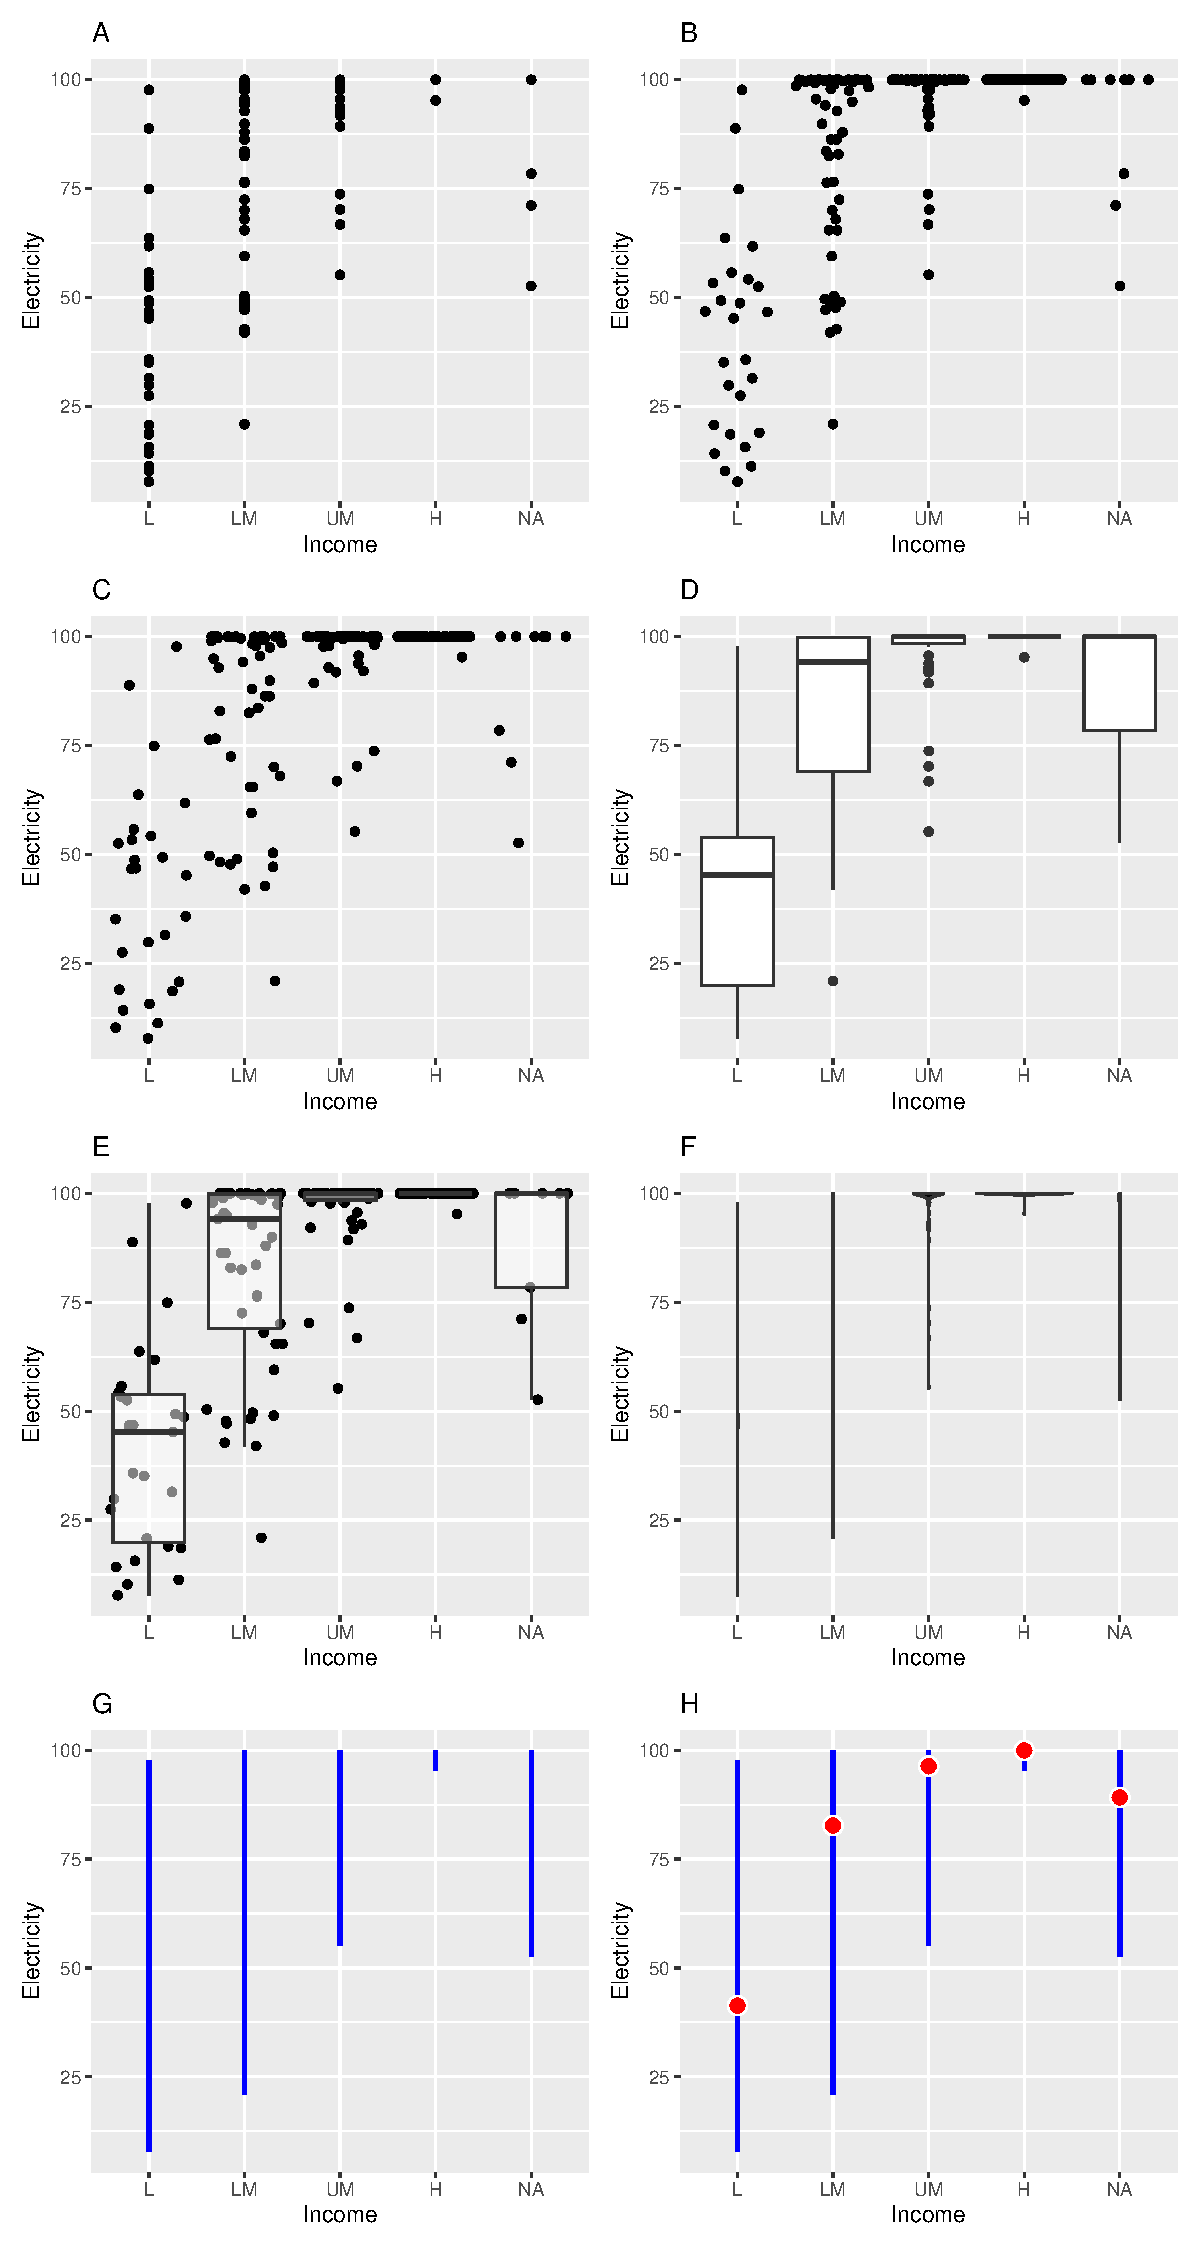
\includegraphics{intro_files/figure-pdf/unnamed-chunk-1-1.pdf}

Second, the data that we are going to draw the plot. Here, I use
\texttt{worldbankdata} available in the package drone.

\begin{verbatim}
# A tibble: 7,937 x 7
   Country Code  Region                     Year Cooking Electricity Income
   <fct>   <fct> <fct>                     <dbl>   <dbl>       <dbl> <fct> 
 1 Aruba   ABW   Latin America & Caribbean  1990      NA       100   H     
 2 Aruba   ABW   Latin America & Caribbean  2000      NA        91.7 H     
 3 Aruba   ABW   Latin America & Caribbean  2013      NA       100   H     
 4 Aruba   ABW   Latin America & Caribbean  2014      NA       100   H     
 5 Aruba   ABW   Latin America & Caribbean  2015      NA       100   H     
 6 Aruba   ABW   Latin America & Caribbean  2016      NA       100   H     
 7 Aruba   ABW   Latin America & Caribbean  2017      NA       100   H     
 8 Aruba   ABW   Latin America & Caribbean  2018      NA       100   H     
 9 Aruba   ABW   Latin America & Caribbean  2019      NA       100   H     
10 Aruba   ABW   Latin America & Caribbean  2020      NA       100   H     
# i 7,927 more rows
\end{verbatim}

Step 2: Map the variables to the graphical properties.

\includegraphics{intro_files/figure-pdf/unnamed-chunk-3-1.pdf}

Step 3: Plot the data.

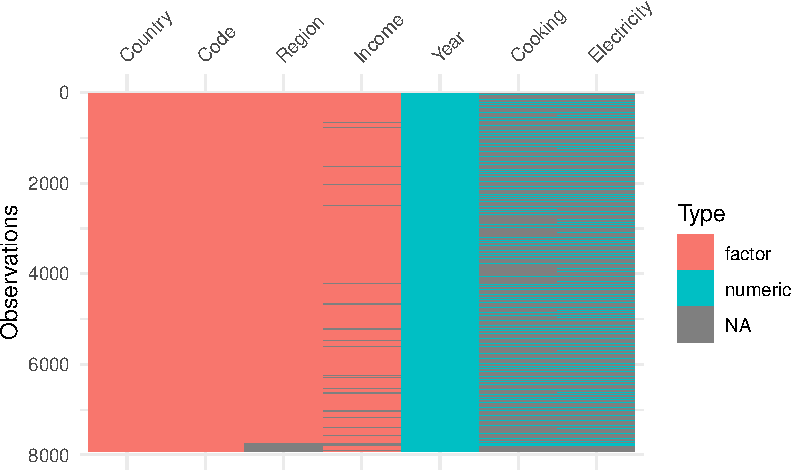
\includegraphics{intro_files/figure-pdf/unnamed-chunk-4-1.pdf}

\section{\texorpdfstring{What is
\texttt{geom}?}{What is geom?}}\label{what-is-geom}

Below are four methods that I used to visualise the distribution of var1
by var 2.

\section{Data}\label{data}

\begin{Shaded}
\begin{Highlighting}[]
\FunctionTok{library}\NormalTok{(drone)}
\FunctionTok{library}\NormalTok{(tibble)}
\FunctionTok{data}\NormalTok{(worldbankdata)}
\NormalTok{worldbankdata}
\end{Highlighting}
\end{Shaded}

\begin{verbatim}
# A tibble: 7,937 x 7
   Country Code  Region                     Year Cooking Electricity Income
   <fct>   <fct> <fct>                     <dbl>   <dbl>       <dbl> <fct> 
 1 Aruba   ABW   Latin America & Caribbean  1990      NA       100   H     
 2 Aruba   ABW   Latin America & Caribbean  2000      NA        91.7 H     
 3 Aruba   ABW   Latin America & Caribbean  2013      NA       100   H     
 4 Aruba   ABW   Latin America & Caribbean  2014      NA       100   H     
 5 Aruba   ABW   Latin America & Caribbean  2015      NA       100   H     
 6 Aruba   ABW   Latin America & Caribbean  2016      NA       100   H     
 7 Aruba   ABW   Latin America & Caribbean  2017      NA       100   H     
 8 Aruba   ABW   Latin America & Caribbean  2018      NA       100   H     
 9 Aruba   ABW   Latin America & Caribbean  2019      NA       100   H     
10 Aruba   ABW   Latin America & Caribbean  2020      NA       100   H     
# i 7,927 more rows
\end{verbatim}

\section{Data description}\label{data-description}

\begin{Shaded}
\begin{Highlighting}[]
\FunctionTok{library}\NormalTok{(tidyverse)}
\FunctionTok{library}\NormalTok{(visdat)}
\FunctionTok{vis\_dat}\NormalTok{(worldbankdata) }\SpecialCharTok{+} 
  \FunctionTok{scale\_fill\_brewer}\NormalTok{(}\AttributeTok{palette =} \StringTok{"Dark2"}\NormalTok{)}
\end{Highlighting}
\end{Shaded}

\includegraphics{intro_files/figure-pdf/unnamed-chunk-6-1.pdf}

\begin{Shaded}
\begin{Highlighting}[]
\FunctionTok{library}\NormalTok{(naniar)}
\FunctionTok{gg\_miss\_upset}\NormalTok{(worldbankdata) }
\end{Highlighting}
\end{Shaded}

\includegraphics{intro_files/figure-pdf/unnamed-chunk-7-1.pdf}

\section{Packages use for data wrangiling and \textbar\textgreater{}
operator}\label{packages-use-for-data-wrangiling-and-operator}

\section{R packages with geom
implementation}\label{r-packages-with-geom-implementation}

\begin{enumerate}
\def\labelenumi{\arabic{enumi}.}
\item
  ggplot2 (Wickham 2016)
\item
  ggpattern (FC, Davis, and ggplot2 authors 2023)
\item
  ggforce (Pedersen 2022)
\item
  ggalluvial (\textbf{ggalluvial?})
\item
  ggbump (Sjoberg 2020)
\item
  ggridges (Wilke 2023)
\item
  ggalt (Rudis, Bolker, and Schulz 2017)
\end{enumerate}

\part{A}

In this part of the book we will look at the geoms starts with letter
``a'' or ``A''.

\begin{longtable}[]{@{}lr@{}}
\toprule\noalign{}
geom & section \\
\midrule\noalign{}
\endhead
\bottomrule\noalign{}
\endlastfoot
geom\_area & 3.1 \\
geom\_abline & 3.2 \\
geom\_alluvium & 3.3 \\
geom\_arc & 3.4 \\
geom\_arc\_bar & 3.5 \\
\end{longtable}

\chapter{geom\_a}\label{sec-a}

\section{geom\_area}\label{area}

\textbf{Package}

ggplot2 (Wickham 2016)

\textbf{Description}

Create an area plot. This cover the space between x-axis and line that
connects the data points.

\textbf{Understandable aesthetics}

\emph{required aesthetics}

\texttt{x}, \texttt{y}

\emph{optional aesthetics}

\texttt{alpha}, \texttt{colour}, \texttt{fill}, \texttt{group},
\texttt{linetype}, \texttt{linewidth}

\textbf{See also}

\hyperref[line]{geom\_line}, \hyperref[ribbon]{geom\_ribbon}

\textbf{Example}

\begin{Shaded}
\begin{Highlighting}[]
\NormalTok{a1 }\OtherTok{\textless{}{-}}\NormalTok{ worldbankdata }\SpecialCharTok{|\textgreater{}}
  \FunctionTok{filter}\NormalTok{(Country }\SpecialCharTok{==} \StringTok{"Bangladesh"}\NormalTok{) }\SpecialCharTok{|\textgreater{}}
  \FunctionTok{filter}\NormalTok{(Year }\SpecialCharTok{\textgreater{}=} \DecValTok{2013} \SpecialCharTok{\&}\NormalTok{ Year }\SpecialCharTok{\textless{}=} \DecValTok{2021}\NormalTok{) }\SpecialCharTok{|\textgreater{}}
  \FunctionTok{ggplot}\NormalTok{(}\FunctionTok{aes}\NormalTok{(}\AttributeTok{x =}\NormalTok{ Year, }\AttributeTok{y =}\NormalTok{ Electricity)) }\SpecialCharTok{+}
  \FunctionTok{geom\_area}\NormalTok{(}\AttributeTok{alpha =} \FloatTok{0.5}\NormalTok{) }\SpecialCharTok{+}
  \FunctionTok{theme}\NormalTok{(}\AttributeTok{axis.text.x =} \FunctionTok{element\_text}\NormalTok{(}\AttributeTok{angle =} \DecValTok{90}\NormalTok{, }\AttributeTok{vjust =} \FloatTok{0.5}\NormalTok{, }\AttributeTok{hjust =} \DecValTok{1}\NormalTok{)) }\SpecialCharTok{+}
  \FunctionTok{scale\_x\_continuous}\NormalTok{(}\AttributeTok{breaks =} \DecValTok{2013}\SpecialCharTok{:}\DecValTok{2021}\NormalTok{) }\SpecialCharTok{+}
  \FunctionTok{labs}\NormalTok{(}\AttributeTok{title =} \StringTok{"a1: geom\_area only"}\NormalTok{)}

\NormalTok{a2 }\OtherTok{\textless{}{-}}\NormalTok{ worldbankdata }\SpecialCharTok{|\textgreater{}}
  \FunctionTok{filter}\NormalTok{(Country }\SpecialCharTok{==} \StringTok{"Bangladesh"}\NormalTok{) }\SpecialCharTok{|\textgreater{}}
  \FunctionTok{filter}\NormalTok{(Year }\SpecialCharTok{\textgreater{}=} \DecValTok{2013} \SpecialCharTok{\&}\NormalTok{ Year }\SpecialCharTok{\textless{}=} \DecValTok{2021}\NormalTok{) }\SpecialCharTok{|\textgreater{}}
  \FunctionTok{ggplot}\NormalTok{(}\FunctionTok{aes}\NormalTok{(}\AttributeTok{x =}\NormalTok{ Year, }\AttributeTok{y =}\NormalTok{ Electricity)) }\SpecialCharTok{+}
  \FunctionTok{geom\_area}\NormalTok{(}\AttributeTok{alpha =} \FloatTok{0.5}\NormalTok{) }\SpecialCharTok{+}
  \FunctionTok{theme}\NormalTok{(}\AttributeTok{axis.text.x =} \FunctionTok{element\_text}\NormalTok{(}\AttributeTok{angle =} \DecValTok{90}\NormalTok{, }\AttributeTok{vjust =} \FloatTok{0.5}\NormalTok{, }\AttributeTok{hjust =} \DecValTok{1}\NormalTok{)) }\SpecialCharTok{+}
  \FunctionTok{scale\_x\_continuous}\NormalTok{(}\AttributeTok{breaks =} \DecValTok{2013}\SpecialCharTok{:}\DecValTok{2021}\NormalTok{) }\SpecialCharTok{+}
  \FunctionTok{geom\_point}\NormalTok{(}\AttributeTok{col =} \StringTok{"red"}\NormalTok{) }\SpecialCharTok{+}
  \FunctionTok{labs}\NormalTok{(}\AttributeTok{title =} \StringTok{"a2: geom\_area }\SpecialCharTok{\textbackslash{}n}\StringTok{ and geom\_point"}\NormalTok{)}
\NormalTok{a1 }\SpecialCharTok{|}\NormalTok{ a2}
\end{Highlighting}
\end{Shaded}

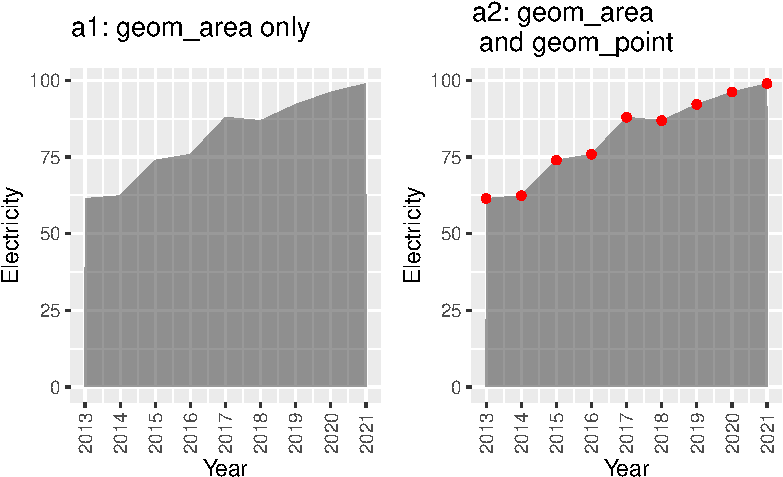
\includegraphics{a_files/figure-pdf/area-1.pdf}

\section{geom\_abline}\label{abline}

\textbf{Package}

ggplot2 (Wickham 2016)

\textbf{Description}

Description Draw a straight line (\(Y=mX+c\)) for a given slope (\(m\))
and intercept (\(c\)).

\textbf{Understandable aesthetics}

Unlike most other geoms, \texttt{geom\_abline} does not depend on the x
and y variables that we map for the main plot. \texttt{geom\_abline} has
its own independent characteristics: \texttt{intercept} and
\texttt{slope}.

\textbf{See also}

\hyperref[point]{geom\_point}, \hyperref[vline]{geom\_vline},
\hyperref[hline]{geom\_hline}

\textbf{Example}

\begin{Shaded}
\begin{Highlighting}[]
\NormalTok{a1 }\OtherTok{\textless{}{-}} \FunctionTok{ggplot}\NormalTok{(worldbankdata, }\FunctionTok{aes}\NormalTok{(}\AttributeTok{y =}\NormalTok{ Cooking, }\AttributeTok{x =}\NormalTok{ Electricity)) }\SpecialCharTok{+}
  \FunctionTok{geom\_abline}\NormalTok{(}\AttributeTok{intercept =} \DecValTok{0}\NormalTok{, }\AttributeTok{slope =} \DecValTok{1}\NormalTok{) }\SpecialCharTok{+}
  \FunctionTok{labs}\NormalTok{(}\AttributeTok{title =} \StringTok{"a1: geom\_abline only"}\NormalTok{) }\SpecialCharTok{+}
  \FunctionTok{theme}\NormalTok{(}\AttributeTok{aspect.ratio =} \DecValTok{1}\NormalTok{)}
\NormalTok{a2 }\OtherTok{\textless{}{-}} \FunctionTok{ggplot}\NormalTok{(worldbankdata, }\FunctionTok{aes}\NormalTok{(}\AttributeTok{y =}\NormalTok{ Cooking, }\AttributeTok{x =}\NormalTok{ Electricity)) }\SpecialCharTok{+}
  \FunctionTok{geom\_abline}\NormalTok{(}\AttributeTok{intercept =} \DecValTok{0}\NormalTok{, }\AttributeTok{slope =} \DecValTok{1}\NormalTok{) }\SpecialCharTok{+}
  \FunctionTok{geom\_point}\NormalTok{() }\SpecialCharTok{+}
  \FunctionTok{labs}\NormalTok{(}\AttributeTok{title =} \StringTok{"a2: geom\_abline }\SpecialCharTok{\textbackslash{}n}\StringTok{ and geom\_point"}\NormalTok{) }\SpecialCharTok{+}
  \FunctionTok{theme}\NormalTok{(}\AttributeTok{aspect.ratio =} \DecValTok{1}\NormalTok{)}
\NormalTok{a1 }\SpecialCharTok{|}\NormalTok{ a2}
\end{Highlighting}
\end{Shaded}

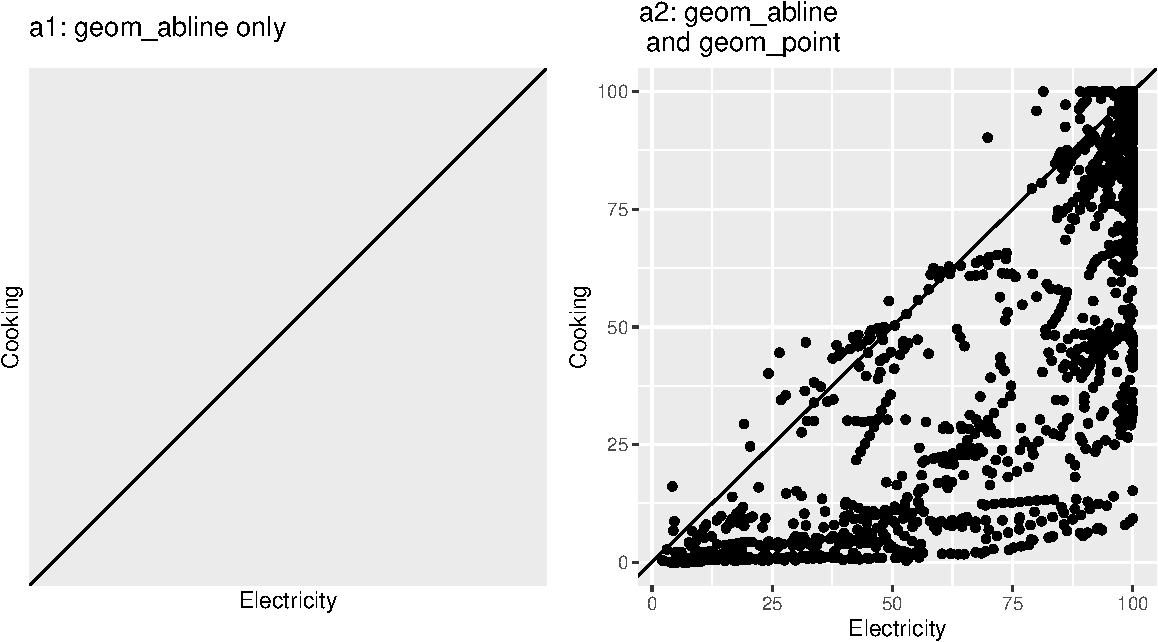
\includegraphics{a_files/figure-pdf/unnamed-chunk-2-1.pdf}

\section{geom\_alluvium}\label{alluvium}

\textbf{Package}

ggalluvial(Brunson and Read 2019; Brunson 2020)

\textbf{Description}

Create alluvial plot. An alluvial plot is a type of diagram that is
particularly useful for visualizing categorical data and the flow or
transition between different categorical variables over multiple stages
or categories

\textbf{Understandable aesthetics}

\emph{required aesthetics}

\texttt{x}, \texttt{y}, \texttt{ymin}, \texttt{ymax},

\emph{optional aesthetics}

\texttt{alpha}, \texttt{colour}, \texttt{fill}, \texttt{linetype},
\texttt{size}, \texttt{group} (group is used internally; arguments are
ignored)

\textbf{See also}

\hyperref[stratum]{geom\_stratum}, \hyperref[flow]{geom\_flow},
\hyperref[lode]{geom\_lode}

\textbf{Example}

\begin{Shaded}
\begin{Highlighting}[]
\FunctionTok{library}\NormalTok{(ggalluvial)}
\NormalTok{freq.table }\OtherTok{\textless{}{-}}\NormalTok{ worldbankdata }\SpecialCharTok{|\textgreater{}}
  \FunctionTok{select}\NormalTok{(Country, Region, Year, Income) }\SpecialCharTok{|\textgreater{}}
  \FunctionTok{filter}\NormalTok{(Year }\SpecialCharTok{\textgreater{}} \DecValTok{2015}\NormalTok{) }\SpecialCharTok{|\textgreater{}}
  \FunctionTok{group\_by}\NormalTok{(Region, Year, Income) }\SpecialCharTok{|\textgreater{}}
  \FunctionTok{summarise}\NormalTok{(}\AttributeTok{n =} \FunctionTok{n}\NormalTok{()) }\SpecialCharTok{|\textgreater{}}
  \FunctionTok{drop\_na}\NormalTok{()}
\NormalTok{freq.table}
\end{Highlighting}
\end{Shaded}

\begin{verbatim}
# A tibble: 153 x 4
# Groups:   Region, Year [49]
   Region               Year Income     n
   <fct>               <dbl> <fct>  <int>
 1 East Asia & Pacific  2016 LM        13
 2 East Asia & Pacific  2016 UM        10
 3 East Asia & Pacific  2016 H         14
 4 East Asia & Pacific  2017 LM        13
 5 East Asia & Pacific  2017 UM        10
 6 East Asia & Pacific  2017 H         14
 7 East Asia & Pacific  2018 LM        13
 8 East Asia & Pacific  2018 UM        10
 9 East Asia & Pacific  2018 H         14
10 East Asia & Pacific  2019 LM        12
# i 143 more rows
\end{verbatim}

\begin{Shaded}
\begin{Highlighting}[]
\NormalTok{a1 }\OtherTok{\textless{}{-}}\NormalTok{ freq.table }\SpecialCharTok{|\textgreater{}}
  \FunctionTok{ggplot}\NormalTok{(}\FunctionTok{aes}\NormalTok{(}\AttributeTok{y =}\NormalTok{ n, }\AttributeTok{axis1 =}\NormalTok{ Region, }\AttributeTok{axis2 =}\NormalTok{ Year)) }\SpecialCharTok{+}
  \FunctionTok{geom\_alluvium}\NormalTok{(}\FunctionTok{aes}\NormalTok{(}\AttributeTok{fill =}\NormalTok{ Income), }\AttributeTok{width =} \DecValTok{1} \SpecialCharTok{/} \DecValTok{12}\NormalTok{) }\SpecialCharTok{+}
  \FunctionTok{labs}\NormalTok{(}\AttributeTok{title =} \StringTok{"a1: geom\_alluvium only"}\NormalTok{)}

\NormalTok{a2 }\OtherTok{\textless{}{-}}\NormalTok{ freq.table }\SpecialCharTok{|\textgreater{}}
  \FunctionTok{ggplot}\NormalTok{(}\FunctionTok{aes}\NormalTok{(}\AttributeTok{y =}\NormalTok{ n, }\AttributeTok{axis1 =}\NormalTok{ Region, }\AttributeTok{axis2 =}\NormalTok{ Year)) }\SpecialCharTok{+}
  \FunctionTok{geom\_alluvium}\NormalTok{(}\FunctionTok{aes}\NormalTok{(}\AttributeTok{fill =}\NormalTok{ Income), }\AttributeTok{width =} \DecValTok{1} \SpecialCharTok{/} \DecValTok{12}\NormalTok{) }\SpecialCharTok{+}
  \FunctionTok{geom\_stratum}\NormalTok{(}\AttributeTok{width =} \DecValTok{1} \SpecialCharTok{/} \DecValTok{12}\NormalTok{, }\AttributeTok{fill =} \StringTok{"black"}\NormalTok{, }\AttributeTok{color =} \StringTok{"grey"}\NormalTok{) }\SpecialCharTok{+}
  \FunctionTok{geom\_label}\NormalTok{(}\AttributeTok{stat =} \StringTok{"stratum"}\NormalTok{, }\FunctionTok{aes}\NormalTok{(}\AttributeTok{label =} \FunctionTok{after\_stat}\NormalTok{(stratum))) }\SpecialCharTok{+}
  \FunctionTok{labs}\NormalTok{(}\AttributeTok{title =} \StringTok{"a2: geom\_alluvium, }\SpecialCharTok{\textbackslash{}n}\StringTok{ geom\_stratum and geom\_label"}\NormalTok{)}
\NormalTok{a1 }\SpecialCharTok{/}\NormalTok{ a2}
\end{Highlighting}
\end{Shaded}

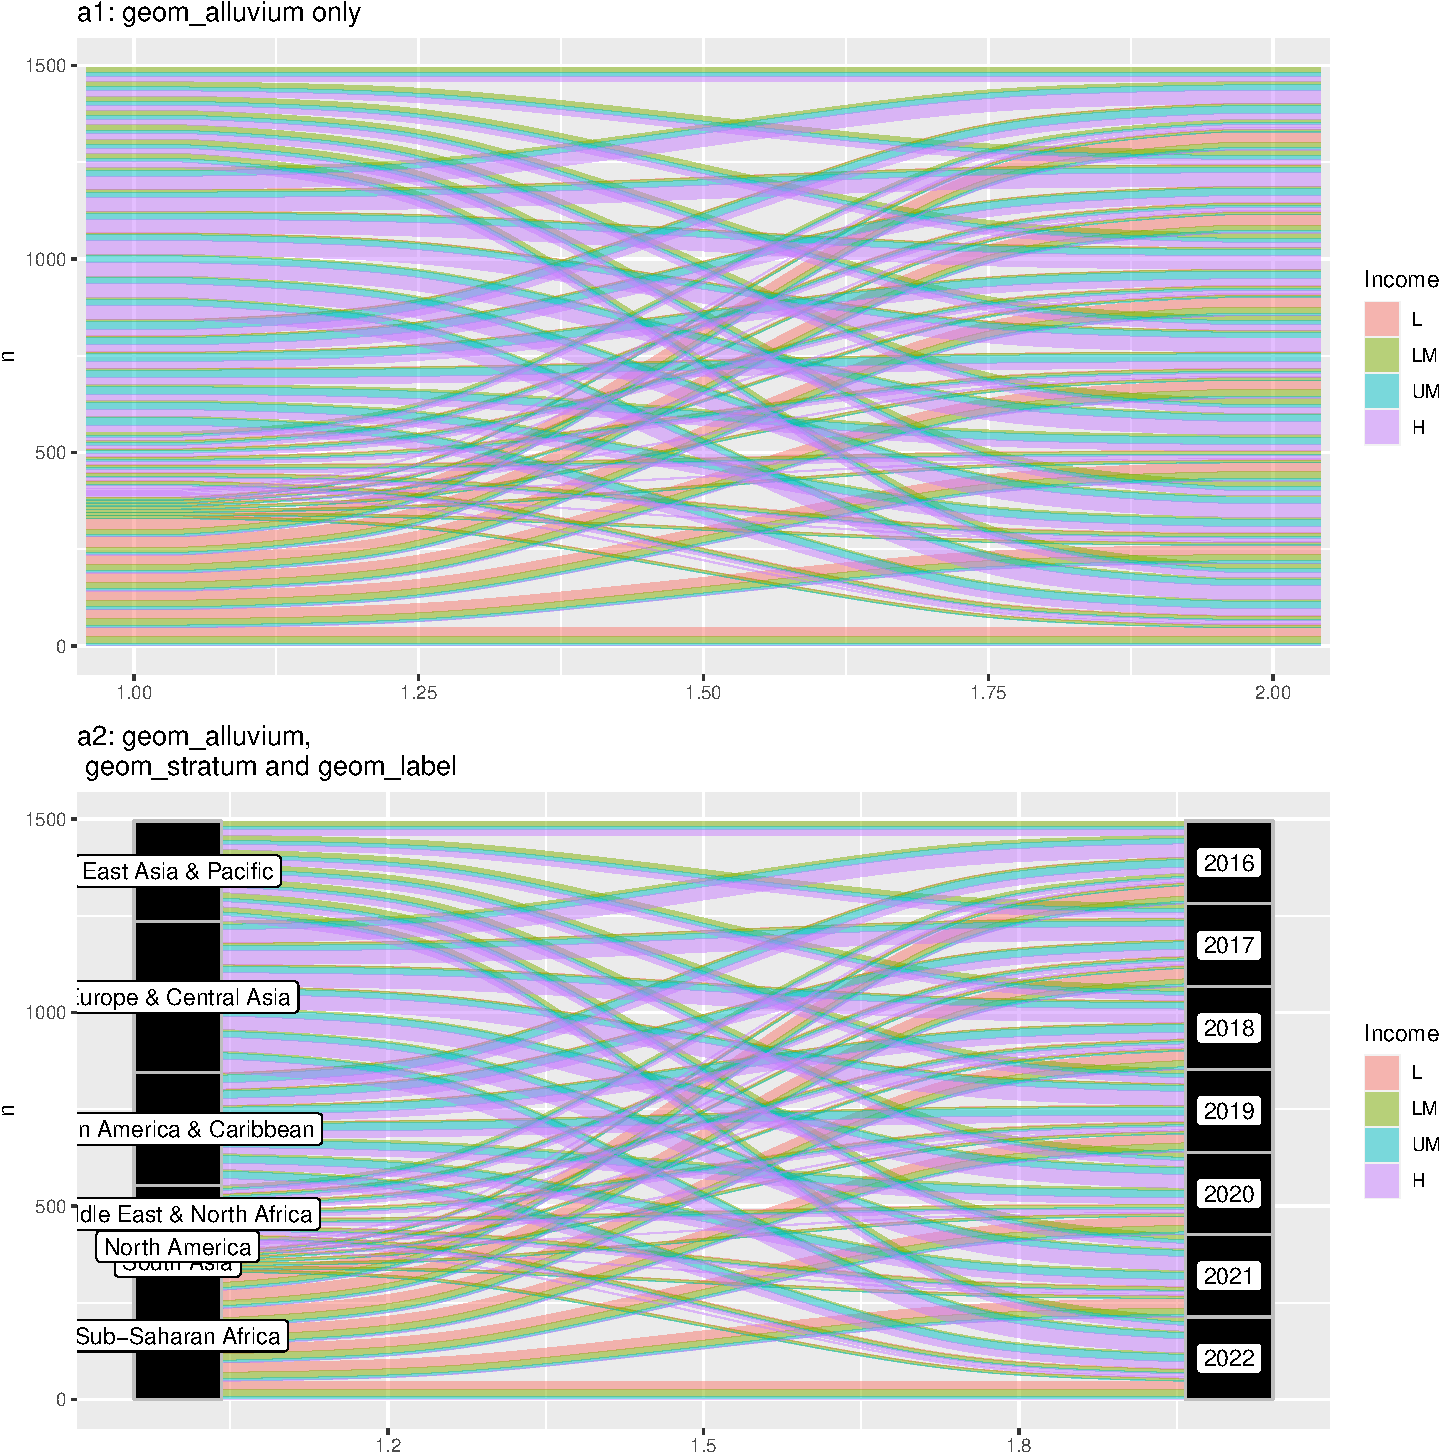
\includegraphics{a_files/figure-pdf/alluvial-1.pdf}

\section{geom\_arc}\label{geom_arc}

\textbf{Package}

ggforce(Pedersen 2022)

\textbf{Description}

Draw a circle or a segment of a circle.

\textbf{Understandable aesthetic}

\emph{required aesthetics}

\texttt{x0} - starting coordinate of x-axis , \texttt{y0} - starting
coordinate of x-axis, \texttt{r} - radius, \texttt{start}, \texttt{end}

\emph{optional aesthetics}

\texttt{color}, \texttt{linewidth}, \texttt{linetype}, \texttt{alpha},
\texttt{lineend}

\textbf{The statistical transformation to use on the data for this
layer}

\texttt{stat\_arc}

\textbf{See also}

\hyperref[arc2]{geom\_arc2}, \hyperref[arcbar]{geom\_arc\_bar}

\textbf{Example}

\begin{Shaded}
\begin{Highlighting}[]
\FunctionTok{library}\NormalTok{(ggforce)}
\FunctionTok{ggplot}\NormalTok{() }\SpecialCharTok{+}
  \FunctionTok{geom\_arc}\NormalTok{(}\FunctionTok{aes}\NormalTok{(}\AttributeTok{x0 =} \DecValTok{0}\NormalTok{, }\AttributeTok{y0 =} \DecValTok{0}\NormalTok{, }\AttributeTok{r =} \DecValTok{8}\NormalTok{, }\AttributeTok{start =} \DecValTok{1}\NormalTok{, }\AttributeTok{end =} \DecValTok{8}\NormalTok{)) }\SpecialCharTok{+}
  \FunctionTok{geom\_arc}\NormalTok{(}\FunctionTok{aes}\NormalTok{(}\AttributeTok{x0 =} \DecValTok{0}\NormalTok{, }\AttributeTok{y0 =} \DecValTok{0}\NormalTok{, }\AttributeTok{r =} \DecValTok{8}\NormalTok{, }\AttributeTok{start =} \DecValTok{1}\NormalTok{, }\AttributeTok{end =} \DecValTok{5}\NormalTok{), }\AttributeTok{col =} \StringTok{"red"}\NormalTok{, }\AttributeTok{size =} \DecValTok{2}\NormalTok{) }\SpecialCharTok{+}
  \FunctionTok{theme}\NormalTok{(}\AttributeTok{aspect.ratio =} \DecValTok{1}\NormalTok{)}
\end{Highlighting}
\end{Shaded}

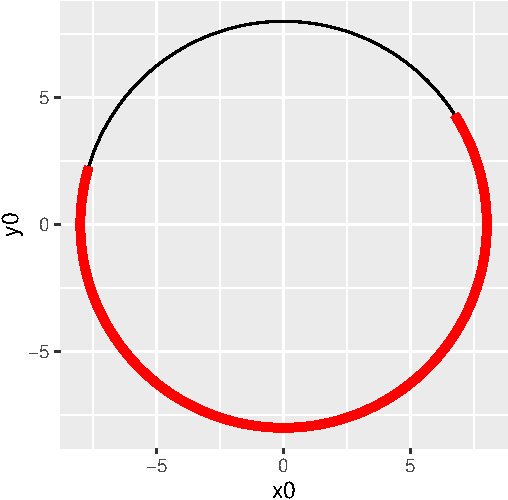
\includegraphics{a_files/figure-pdf/arc-1.pdf}

\section{geom\_arc\_bar}\label{arcbar}

\textbf{Package}

ggforce(Pedersen 2022)

\textbf{Description}

To draw pie chart and donut chart defining centre point, a radius and a
start and end angle.

\textbf{Understandable aesthetic}

\emph{required aesthetics}

\texttt{x0} - starting coordinate of x-axis , \texttt{y0} - starting
coordinate of x-axis, \texttt{r} - radius, \texttt{start}, \texttt{end}

\emph{optional aesthetics}

\texttt{color}, \texttt{linewidth}, \texttt{linetype}, \texttt{alpha},
\texttt{lineend}

\textbf{The statistical transformation to use on the data for this
layer}

\texttt{stat\_arc}

\textbf{See also}

\hyperref[arc]{geom\_arc}, \hyperref[arcbar]{geom\_arc\_bar}

\textbf{Example}

\begin{Shaded}
\begin{Highlighting}[]
\NormalTok{df }\OtherTok{\textless{}{-}} \FunctionTok{data.frame}\NormalTok{(}
  \AttributeTok{state =} \FunctionTok{c}\NormalTok{(}
    \StringTok{"A"}\NormalTok{, }\StringTok{"B"}\NormalTok{, }\StringTok{"C"}\NormalTok{,}
    \StringTok{"D"}\NormalTok{, }\StringTok{"E"}
\NormalTok{  ),}
  \AttributeTok{focus =} \FunctionTok{c}\NormalTok{(}\FloatTok{0.2}\NormalTok{, }\DecValTok{0}\NormalTok{, }\DecValTok{0}\NormalTok{, }\DecValTok{0}\NormalTok{, }\DecValTok{0}\NormalTok{),}
  \AttributeTok{start =} \FunctionTok{c}\NormalTok{(}\DecValTok{0}\NormalTok{, }\DecValTok{1}\NormalTok{, }\DecValTok{2}\NormalTok{, }\DecValTok{3}\NormalTok{, }\DecValTok{4}\NormalTok{),}
  \AttributeTok{end =} \FunctionTok{c}\NormalTok{(}\DecValTok{1}\NormalTok{, }\DecValTok{2}\NormalTok{, }\DecValTok{3}\NormalTok{, }\DecValTok{4}\NormalTok{, }\DecValTok{2} \SpecialCharTok{*}\NormalTok{ pi),}
  \AttributeTok{amount =} \FunctionTok{c}\NormalTok{(}\DecValTok{4}\NormalTok{, }\DecValTok{3}\NormalTok{, }\DecValTok{1}\NormalTok{, }\DecValTok{2}\NormalTok{, }\DecValTok{5}\NormalTok{),}
  \AttributeTok{stringsAsFactors =} \ConstantTok{FALSE}
\NormalTok{)}
\FunctionTok{ggplot}\NormalTok{(df) }\SpecialCharTok{+}
  \FunctionTok{geom\_arc\_bar}\NormalTok{(}\FunctionTok{aes}\NormalTok{(}
    \AttributeTok{x0 =} \DecValTok{0}\NormalTok{, }\AttributeTok{y0 =} \DecValTok{0}\NormalTok{, }\AttributeTok{r0 =} \DecValTok{0}\NormalTok{, }\AttributeTok{r =} \DecValTok{1}\NormalTok{, }\AttributeTok{amount =}\NormalTok{ amount,}
    \AttributeTok{fill =}\NormalTok{ state, }\AttributeTok{explode =}\NormalTok{ focus}
\NormalTok{  ), }\AttributeTok{stat =} \StringTok{"pie"}\NormalTok{) }\SpecialCharTok{+}
  \FunctionTok{scale\_fill\_brewer}\NormalTok{(}\AttributeTok{palette =} \StringTok{"Dark2"}\NormalTok{) }\SpecialCharTok{+}
  \FunctionTok{theme}\NormalTok{(}\AttributeTok{aspect.ratio =} \DecValTok{1}\NormalTok{)}
\end{Highlighting}
\end{Shaded}

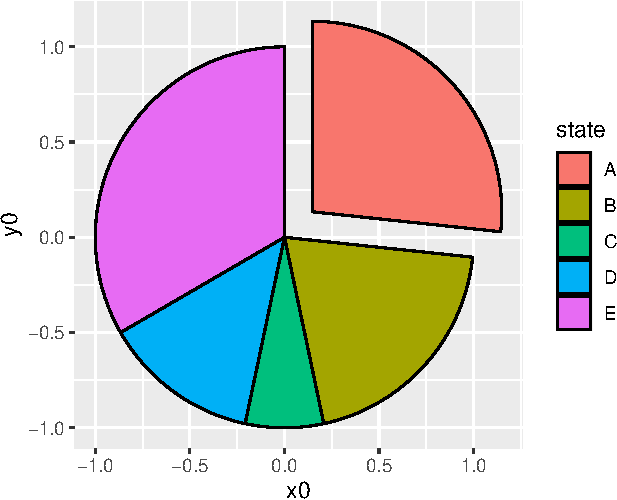
\includegraphics{a_files/figure-pdf/unnamed-chunk-3-1.pdf}

\#\#geom\_arrow\{\#arrow\}

\textbf{Package}

metR (Campitelli 2021)

\textbf{Description}

\textbf{Understandable aesthetics}

\emph{required aesthetics}

\texttt{x}

\texttt{y}

\emph{optional aesthetics}

\texttt{arrow,type}, \texttt{arrow.angle}, \texttt{arrow.length},
\texttt{arrow.ends}, \texttt{arrow.type}

\textbf{See also}

\hyperref[line]{geom\_line}, \hyperref[ribbon]{geom\_ribbon}

\subsection{Example}\label{example}

\begin{Shaded}
\begin{Highlighting}[]
\FunctionTok{library}\NormalTok{(metR)}
\end{Highlighting}
\end{Shaded}

\begin{verbatim}

Attaching package: 'metR'
\end{verbatim}

\begin{verbatim}
The following object is masked from 'package:purrr':

    cross
\end{verbatim}

\begin{Shaded}
\begin{Highlighting}[]
\NormalTok{data }\OtherTok{\textless{}{-}} \FunctionTok{tibble}\NormalTok{(}
  \AttributeTok{x =} \FunctionTok{c}\NormalTok{(}\DecValTok{10}\NormalTok{, }\DecValTok{20}\NormalTok{, }\DecValTok{30}\NormalTok{, }\DecValTok{40}\NormalTok{, }\DecValTok{50}\NormalTok{),           }\CommentTok{\# Longitude or X{-}coordinates}
  \AttributeTok{y =} \FunctionTok{c}\NormalTok{(}\DecValTok{1}\NormalTok{, }\DecValTok{2}\NormalTok{, }\DecValTok{3}\NormalTok{, }\DecValTok{4}\NormalTok{, }\DecValTok{5}\NormalTok{),           }\CommentTok{\# Latitude or Y{-}coordinates}
  \AttributeTok{dx =} \FunctionTok{c}\NormalTok{(}\DecValTok{1}\NormalTok{, }\DecValTok{0}\NormalTok{, }\SpecialCharTok{{-}}\DecValTok{1}\NormalTok{, }\DecValTok{0}\NormalTok{, }\DecValTok{1}\NormalTok{),         }\CommentTok{\# Wind direction components (change in X)}
  \AttributeTok{dy =} \FunctionTok{c}\NormalTok{(}\DecValTok{1}\NormalTok{, }\SpecialCharTok{{-}}\DecValTok{1}\NormalTok{, }\DecValTok{0}\NormalTok{, }\DecValTok{1}\NormalTok{, }\DecValTok{0}\NormalTok{)          }\CommentTok{\# Wind direction components (change in Y)}
\NormalTok{)}

\FunctionTok{ggplot}\NormalTok{(data, }\FunctionTok{aes}\NormalTok{(}\AttributeTok{x =}\NormalTok{ x, }\AttributeTok{y =}\NormalTok{ y)) }\SpecialCharTok{+}
  \FunctionTok{geom\_point}\NormalTok{(}\AttributeTok{color =} \StringTok{"\#1b9e77"}\NormalTok{, }\AttributeTok{size =} \DecValTok{3}\NormalTok{) }\SpecialCharTok{+}  
  \FunctionTok{geom\_arrow}\NormalTok{(}\FunctionTok{aes}\NormalTok{(}\AttributeTok{dx =}\NormalTok{ dx, }\AttributeTok{dy =}\NormalTok{ dy), }\AttributeTok{color =} \StringTok{"\#d95f02"}\NormalTok{, }\AttributeTok{size =} \DecValTok{1}\NormalTok{, }\AttributeTok{arrow.type =} \StringTok{"closed"}\NormalTok{) }\SpecialCharTok{+}
  \FunctionTok{labs}\NormalTok{(}\AttributeTok{title =} \StringTok{"Wind Directions at Different Locations"}\NormalTok{, }\AttributeTok{x =} \StringTok{"Longitude"}\NormalTok{, }\AttributeTok{y =} \StringTok{"Latitude"}\NormalTok{)}
\end{Highlighting}
\end{Shaded}

\includegraphics{a_files/figure-pdf/unnamed-chunk-4-1.pdf}

\section{geom\_ash}\label{ash}

\textbf{Package}

ggformula (Kaplan and Pruim 2023)

\textbf{Description}

Plotted Average Shifted Histogram (ASH)

\textbf{Understandable aesthetics}

\emph{required aesthetics}

\texttt{x}

\texttt{y}

\emph{optional aesthetics}

\texttt{color}, \texttt{fill}, \texttt{bins}, \texttt{alpha},
\texttt{size}

\textbf{See also}

\hyperref[histogram]{geom\_histogram}, \hyperref[density]{geom\_density}

\textbf{Example}

\begin{Shaded}
\begin{Highlighting}[]
\FunctionTok{library}\NormalTok{(ggformula)}
\NormalTok{p1 }\OtherTok{\textless{}{-}}\NormalTok{ worldbankdata }\SpecialCharTok{|\textgreater{}}
  \FunctionTok{filter}\NormalTok{(Income }\SpecialCharTok{==} \StringTok{"LM"}\NormalTok{) }\SpecialCharTok{|\textgreater{}}
  \FunctionTok{ggplot}\NormalTok{(}\FunctionTok{aes}\NormalTok{(}\AttributeTok{x =}\NormalTok{ Electricity)) }\SpecialCharTok{+}
   \FunctionTok{geom\_ash}\NormalTok{(}\AttributeTok{bins =} \DecValTok{20}\NormalTok{, }\AttributeTok{color =} \StringTok{"\#d95f02"}\NormalTok{) }\SpecialCharTok{+} \FunctionTok{labs}\NormalTok{(}\StringTok{"Average Shifted Histogram"}\NormalTok{)}
\NormalTok{p2 }\OtherTok{\textless{}{-}}\NormalTok{ worldbankdata }\SpecialCharTok{|\textgreater{}}
  \FunctionTok{filter}\NormalTok{(Income }\SpecialCharTok{==} \StringTok{"LM"}\NormalTok{) }\SpecialCharTok{|\textgreater{}}
  \FunctionTok{ggplot}\NormalTok{(}\FunctionTok{aes}\NormalTok{(}\AttributeTok{x =}\NormalTok{ Electricity)) }\SpecialCharTok{+}
  \FunctionTok{geom\_histogram}\NormalTok{(}\FunctionTok{aes}\NormalTok{(}\AttributeTok{y =} \FunctionTok{stat}\NormalTok{(density)), }\AttributeTok{color =} \StringTok{"black"}\NormalTok{, }\AttributeTok{fill =} \StringTok{"gray"}\NormalTok{) }\SpecialCharTok{+}
   \FunctionTok{geom\_ash}\NormalTok{(}\AttributeTok{bins =} \DecValTok{20}\NormalTok{, }\AttributeTok{color =} \StringTok{"\#d95f02"}\NormalTok{) }\SpecialCharTok{+} \FunctionTok{labs}\NormalTok{(}\StringTok{"Histogram and Average Shifted Histogram"}\NormalTok{)}
\NormalTok{p1}\SpecialCharTok{|}\NormalTok{p2}
\end{Highlighting}
\end{Shaded}

\includegraphics{a_files/figure-pdf/unnamed-chunk-5-1.pdf}

\part{B}

In this part of the book we will look at the geoms starts with letter
``b'' or ``B''.

\begin{longtable}[]{@{}lr@{}}
\toprule\noalign{}
geom & section \\
\midrule\noalign{}
\endhead
\bottomrule\noalign{}
\endlastfoot
geom\_bar & 4.1 \\
geom\_bin\_2d & 4.2 \\
geom\_bin2d\_pattern & 4.3 \\
geom\_bin2d & 4.4 \\
geom\_blank & 4.5 \\
geom\_boxplot & 4.6 \\
\end{longtable}

\chapter{geom\_b}\label{sec-b}

\section{geom\_bar}\label{bar}

\textbf{Package}

ggplot2 (Wickham 2016)

\textbf{Description}

Draw a bar proportional to the specified number. For example, number of
cases or user defined number.

\textbf{Understandable aesthetics}

\emph{required aesthetics}

\texttt{x}, \texttt{y},

\emph{optional aesthetics}

\texttt{alpha}, \texttt{colour}, \texttt{fill}, \texttt{group},
\texttt{linetype}, \texttt{linewidth}

\textbf{See also}

\hyperref[col]{geom\_col}

\textbf{Example}

\emph{Example 1: Given observations}

\begin{Shaded}
\begin{Highlighting}[]
\NormalTok{worldbankdata }\SpecialCharTok{|\textgreater{}}
\NormalTok{  dplyr}\SpecialCharTok{::}\FunctionTok{select}\NormalTok{(}\FunctionTok{c}\NormalTok{(}\StringTok{"Year"}\NormalTok{, }\StringTok{"Income"}\NormalTok{)) }\SpecialCharTok{|\textgreater{}}
\NormalTok{  dplyr}\SpecialCharTok{::}\FunctionTok{filter}\NormalTok{(Year }\SpecialCharTok{==} \DecValTok{2021}\NormalTok{) }\SpecialCharTok{|\textgreater{}}
  \FunctionTok{ggplot}\NormalTok{(}\FunctionTok{aes}\NormalTok{(}\AttributeTok{x =}\NormalTok{ Income)) }\SpecialCharTok{+}
  \FunctionTok{geom\_bar}\NormalTok{()}
\end{Highlighting}
\end{Shaded}

\includegraphics{b_files/figure-pdf/unnamed-chunk-2-1.pdf}

\emph{Example 2}

\begin{Shaded}
\begin{Highlighting}[]
\NormalTok{worldbankdata }\SpecialCharTok{|\textgreater{}}
\NormalTok{  dplyr}\SpecialCharTok{::}\FunctionTok{select}\NormalTok{(}\FunctionTok{c}\NormalTok{(}\StringTok{"Year"}\NormalTok{, }\StringTok{"Income"}\NormalTok{, }\StringTok{"Region"}\NormalTok{)) }\SpecialCharTok{|\textgreater{}}
\NormalTok{  dplyr}\SpecialCharTok{::}\FunctionTok{filter}\NormalTok{(Year }\SpecialCharTok{==} \DecValTok{2021}\NormalTok{) }\SpecialCharTok{|\textgreater{}}
  \FunctionTok{ggplot}\NormalTok{(}\FunctionTok{aes}\NormalTok{(}\AttributeTok{x =}\NormalTok{ Income, }\AttributeTok{fill =}\NormalTok{ Region)) }\SpecialCharTok{+}
  \FunctionTok{geom\_bar}\NormalTok{() }\SpecialCharTok{+}
  \FunctionTok{scale\_fill\_brewer}\NormalTok{(}\AttributeTok{palette =} \StringTok{"Paired"}\NormalTok{, }\AttributeTok{na.value =} \StringTok{"grey50"}\NormalTok{)}
\end{Highlighting}
\end{Shaded}

\includegraphics{b_files/figure-pdf/unnamed-chunk-3-1.pdf}

\emph{Example 3}

\begin{Shaded}
\begin{Highlighting}[]
\NormalTok{worldbankdata }\SpecialCharTok{|\textgreater{}}
\NormalTok{  dplyr}\SpecialCharTok{::}\FunctionTok{select}\NormalTok{(}\FunctionTok{c}\NormalTok{(}\StringTok{"Year"}\NormalTok{, }\StringTok{"Income"}\NormalTok{, }\StringTok{"Region"}\NormalTok{)) }\SpecialCharTok{|\textgreater{}}
\NormalTok{  dplyr}\SpecialCharTok{::}\FunctionTok{filter}\NormalTok{(Year }\SpecialCharTok{==} \DecValTok{2021}\NormalTok{) }\SpecialCharTok{|\textgreater{}}
  \FunctionTok{ggplot}\NormalTok{(}\FunctionTok{aes}\NormalTok{(}\AttributeTok{x =}\NormalTok{ Income, }\AttributeTok{fill =}\NormalTok{ Region)) }\SpecialCharTok{+}
  \FunctionTok{geom\_bar}\NormalTok{(}\AttributeTok{position =} \StringTok{"dodge"}\NormalTok{) }\SpecialCharTok{+}
  \FunctionTok{scale\_fill\_brewer}\NormalTok{(}\AttributeTok{palette =} \StringTok{"Paired"}\NormalTok{, }\AttributeTok{na.value =} \StringTok{"grey50"}\NormalTok{)}
\end{Highlighting}
\end{Shaded}

\includegraphics{b_files/figure-pdf/unnamed-chunk-4-1.pdf}

\emph{Example 4: Given counts}

\begin{Shaded}
\begin{Highlighting}[]
\NormalTok{dfbar }\OtherTok{\textless{}{-}} \FunctionTok{data.frame}\NormalTok{(}\AttributeTok{class =} \FunctionTok{c}\NormalTok{(}\StringTok{"A"}\NormalTok{, }\StringTok{"B"}\NormalTok{), }\AttributeTok{income =} \FunctionTok{c}\NormalTok{(}\DecValTok{100}\NormalTok{, }\DecValTok{200}\NormalTok{))}
\FunctionTok{ggplot}\NormalTok{(dfbar, }\FunctionTok{aes}\NormalTok{(class, income)) }\SpecialCharTok{+}
  \FunctionTok{geom\_bar}\NormalTok{(}\AttributeTok{stat =} \StringTok{"identity"}\NormalTok{)}
\end{Highlighting}
\end{Shaded}

\includegraphics{b_files/figure-pdf/unnamed-chunk-5-1.pdf}

\section{geom\_bar\_pattern}\label{bar_pattern}

\textbf{Package}

ggpattern (FC, Davis, and ggplot2 authors 2023)

\textbf{Description}

Fill bars with patterns

\textbf{Understandable aesthetics}

\emph{required aesthetics}

\texttt{x}, \texttt{y},

\emph{optional aesthetics}

\texttt{pattern}, \texttt{pattern\_angle}

\textbf{See also}

\hyperref[bar]{geom\_bar}

\textbf{Example}

\begin{Shaded}
\begin{Highlighting}[]
\FunctionTok{library}\NormalTok{(ggpattern)}
\NormalTok{worldbankdata }\SpecialCharTok{|\textgreater{}}
\NormalTok{  tidyr}\SpecialCharTok{::}\FunctionTok{drop\_na}\NormalTok{() }\SpecialCharTok{|\textgreater{}} \DocumentationTok{\#\# Missing values should be removed to see the different patterns for different levels}
\NormalTok{  dplyr}\SpecialCharTok{::}\FunctionTok{select}\NormalTok{(}\FunctionTok{c}\NormalTok{(}\StringTok{"Year"}\NormalTok{, }\StringTok{"Income"}\NormalTok{)) }\SpecialCharTok{|\textgreater{}}
\NormalTok{  dplyr}\SpecialCharTok{::}\FunctionTok{filter}\NormalTok{(Year }\SpecialCharTok{==} \DecValTok{2021}\NormalTok{) }\SpecialCharTok{|\textgreater{}}
  \FunctionTok{ggplot}\NormalTok{(}\FunctionTok{aes}\NormalTok{(}\AttributeTok{x =}\NormalTok{ Income)) }\SpecialCharTok{+}
  \FunctionTok{geom\_bar\_pattern}\NormalTok{(}\FunctionTok{aes}\NormalTok{(}\AttributeTok{pattern =}\NormalTok{ Income, }\AttributeTok{pattern\_angle =}\NormalTok{ Income), }\AttributeTok{fill =} \StringTok{"white"}\NormalTok{, }\AttributeTok{colour =} \StringTok{"black"}\NormalTok{, }\AttributeTok{pattern\_spacing =} \FloatTok{0.03}\NormalTok{, }\AttributeTok{pattern\_key\_scale\_factor =} \DecValTok{1}\NormalTok{)}
\end{Highlighting}
\end{Shaded}

\includegraphics{b_files/figure-pdf/unnamed-chunk-6-1.pdf}

\section{geom\_bin\_2d}\label{bin2d}

\textbf{Package}

ggplot2 (Wickham 2016)

\textbf{Description}

Divides the Cartesian plane created by x-variable and y-variable into
rectangles (2D histogram), counts the number of observations in each
rectangle. Only the observations with rectangles are filled according to
the number of observations.

\textbf{Understandable aesthetics}

\textbf{required aesthetics}

\texttt{x}, \texttt{y},

\textbf{optional aesthetics}

\texttt{fill}, \texttt{group}

\textbf{See also}

\hyperref[bin2d]{geom\_bin2d}, \hyperref[point]{geom\_point}

\textbf{Example}

\begin{Shaded}
\begin{Highlighting}[]
\FunctionTok{ggplot}\NormalTok{(worldbankdata, }\FunctionTok{aes}\NormalTok{(}\AttributeTok{y =}\NormalTok{ Cooking, }\AttributeTok{x =}\NormalTok{ Electricity)) }\SpecialCharTok{+}
  \FunctionTok{geom\_bin\_2d}\NormalTok{() }\SpecialCharTok{+}
  \FunctionTok{scale\_fill\_viridis}\NormalTok{(}\AttributeTok{na.value =} \StringTok{"grey50"}\NormalTok{, }\AttributeTok{limits =} \FunctionTok{c}\NormalTok{(}\DecValTok{0}\NormalTok{, }\DecValTok{30}\NormalTok{)) }\SpecialCharTok{+}
  \FunctionTok{theme}\NormalTok{(}\AttributeTok{aspect.ratio =} \DecValTok{1}\NormalTok{)}
\end{Highlighting}
\end{Shaded}

\includegraphics{b_files/figure-pdf/unnamed-chunk-7-1.pdf}

\begin{Shaded}
\begin{Highlighting}[]
\FunctionTok{ggplot}\NormalTok{(worldbankdata, }\FunctionTok{aes}\NormalTok{(}\AttributeTok{y =}\NormalTok{ Cooking, }\AttributeTok{x =}\NormalTok{ Electricity)) }\SpecialCharTok{+}
  \FunctionTok{geom\_bin\_2d}\NormalTok{(}\AttributeTok{bins =} \DecValTok{20}\NormalTok{) }\SpecialCharTok{+}
  \FunctionTok{scale\_fill\_viridis}\NormalTok{(}\AttributeTok{na.value =} \StringTok{"grey50"}\NormalTok{, }\AttributeTok{limits =} \FunctionTok{c}\NormalTok{(}\DecValTok{0}\NormalTok{, }\DecValTok{30}\NormalTok{)) }\SpecialCharTok{+}
  \FunctionTok{theme}\NormalTok{(}\AttributeTok{aspect.ratio =} \DecValTok{1}\NormalTok{)}
\end{Highlighting}
\end{Shaded}

\includegraphics{b_files/figure-pdf/unnamed-chunk-8-1.pdf}

\section{geom\_bin2d\_pattern}\label{bin2dpattern}

\textbf{Package}

ggpattern(FC, Davis, and ggplot2 authors 2023)

\textbf{Description}

Divides the Cartesian plane created by x-variable and y-variable into
rectangles (2D-Histogram), counts the number of observations in each
rectangle. Only the observations with rectangles are filled with a
pattern.

\textbf{Understandable aesthetics}

\emph{Required aesthetics}

\texttt{x}, \texttt{y}

\emph{Optional aesthetics}

\texttt{pattern\_fill} (pattern\_* - for mapping variables under
aesthetics), \texttt{pattern} (to set a patten, for example
pattern=`stripe'), \texttt{fill}, \texttt{colour}

\textbf{See also}

\hyperref[bin2d]{geom\_bin2d}, \hyperref[point]{geom\_point}

\textbf{Example}

\begin{Shaded}
\begin{Highlighting}[]
\NormalTok{worldbankdata }\SpecialCharTok{|\textgreater{}}
  \FunctionTok{drop\_na}\NormalTok{() }\SpecialCharTok{|\textgreater{}}
  \FunctionTok{ggplot}\NormalTok{(}\FunctionTok{aes}\NormalTok{(}\AttributeTok{y =}\NormalTok{ Cooking, }\AttributeTok{x =}\NormalTok{ Electricity)) }\SpecialCharTok{+}
  \FunctionTok{geom\_bin2d\_pattern}\NormalTok{(}\FunctionTok{aes}\NormalTok{(}\AttributeTok{pattern\_spacing =}\NormalTok{ ..density..), }\AttributeTok{fill =} \StringTok{"white"}\NormalTok{, }\AttributeTok{colour =} \StringTok{"black"}\NormalTok{, }\AttributeTok{bins =} \DecValTok{20}\NormalTok{) }\SpecialCharTok{+}
  \FunctionTok{theme}\NormalTok{(}\AttributeTok{aspect.ratio =} \DecValTok{1}\NormalTok{)}
\end{Highlighting}
\end{Shaded}

\includegraphics{b_files/figure-pdf/unnamed-chunk-9-1.pdf}

\section{geom\_bin2d}\label{bin2d}

\textbf{Package}

ggplot2 (\textbf{R-ggplot2?})

\textbf{Description}

Divides the Cartesian plane created by x-variable and y-variable into
rectangles, counts the number of observations in each rectangle. Only
the observations with rectangles are filled according to the number of
observations.

\textbf{Understandable aesthetics}

\texttt{x}, \texttt{y}, \texttt{fill}, \texttt{group}

\textbf{See also}

\hyperref[bin_2d]{geom\_bin\_2d}, \hyperref[point]{geom\_point}

\textbf{Example}

\begin{Shaded}
\begin{Highlighting}[]
\FunctionTok{ggplot}\NormalTok{(worldbankdata, }\FunctionTok{aes}\NormalTok{(}\AttributeTok{y =}\NormalTok{ Cooking, }\AttributeTok{x =}\NormalTok{ Electricity)) }\SpecialCharTok{+}
  \FunctionTok{geom\_bin2d}\NormalTok{() }\SpecialCharTok{+}
  \FunctionTok{theme}\NormalTok{(}\AttributeTok{aspect.ratio =} \DecValTok{1}\NormalTok{) }\SpecialCharTok{+}
  \FunctionTok{scale\_fill\_viridis}\NormalTok{(}\AttributeTok{na.value =} \StringTok{"grey50"}\NormalTok{, }\AttributeTok{limits =} \FunctionTok{c}\NormalTok{(}\DecValTok{0}\NormalTok{, }\DecValTok{30}\NormalTok{))}
\end{Highlighting}
\end{Shaded}

\includegraphics{b_files/figure-pdf/unnamed-chunk-10-1.pdf}

\section{geom\_blank}\label{blank}

\textbf{Package}

ggplot2 (\textbf{R-ggplot2?})

\textbf{Description}

Draws nothing.

\section{geom\_boxplot}\label{boxplot}

\textbf{Package}

ggplot2 (\textbf{R-ggplot2?})

\textbf{Description}

Draw a bar proportional to the specified number. For example, number of
cases or user defined number.

\textbf{See also}

\hyperref[col]{geom\_col}

\textbf{Example}

\begin{Shaded}
\begin{Highlighting}[]
\NormalTok{worldbankdata }\SpecialCharTok{|\textgreater{}}
\NormalTok{  dplyr}\SpecialCharTok{::}\FunctionTok{filter}\NormalTok{(Year }\SpecialCharTok{==} \DecValTok{2021}\NormalTok{) }\SpecialCharTok{|\textgreater{}}
\NormalTok{  dplyr}\SpecialCharTok{::}\FunctionTok{select}\NormalTok{(Cooking) }\SpecialCharTok{|\textgreater{}}
  \FunctionTok{ggplot}\NormalTok{(}\FunctionTok{aes}\NormalTok{(}\AttributeTok{y =}\NormalTok{ Cooking, }\AttributeTok{x =} \FunctionTok{factor}\NormalTok{(}\DecValTok{0}\NormalTok{))) }\SpecialCharTok{+}
  \FunctionTok{geom\_boxplot}\NormalTok{() }\SpecialCharTok{+}
  \FunctionTok{theme}\NormalTok{(}
    \AttributeTok{axis.title.x =} \FunctionTok{element\_blank}\NormalTok{(),}
    \AttributeTok{axis.text.x =} \FunctionTok{element\_blank}\NormalTok{(),}
    \AttributeTok{axis.ticks.x =} \FunctionTok{element\_blank}\NormalTok{()}
\NormalTok{  )}
\end{Highlighting}
\end{Shaded}

\includegraphics{b_files/figure-pdf/unnamed-chunk-11-1.pdf}

\begin{Shaded}
\begin{Highlighting}[]
\NormalTok{worldbankdata }\SpecialCharTok{|\textgreater{}}
\NormalTok{  dplyr}\SpecialCharTok{::}\FunctionTok{filter}\NormalTok{(Year }\SpecialCharTok{==} \DecValTok{2021}\NormalTok{) }\SpecialCharTok{|\textgreater{}}
  \FunctionTok{ggplot}\NormalTok{(}\FunctionTok{aes}\NormalTok{(}\AttributeTok{y =}\NormalTok{ Cooking, }\AttributeTok{x =}\NormalTok{ Region)) }\SpecialCharTok{+}
  \FunctionTok{geom\_boxplot}\NormalTok{() }\SpecialCharTok{+}
  \FunctionTok{theme}\NormalTok{(}
    \AttributeTok{axis.title.x =} \FunctionTok{element\_blank}\NormalTok{(),}
    \AttributeTok{axis.text.x =} \FunctionTok{element\_blank}\NormalTok{(),}
    \AttributeTok{axis.ticks.x =} \FunctionTok{element\_blank}\NormalTok{()}
\NormalTok{  )}
\end{Highlighting}
\end{Shaded}

\includegraphics{b_files/figure-pdf/unnamed-chunk-12-1.pdf}

\begin{Shaded}
\begin{Highlighting}[]
\NormalTok{worldbankdata }\SpecialCharTok{|\textgreater{}}
\NormalTok{  dplyr}\SpecialCharTok{::}\FunctionTok{filter}\NormalTok{(Year }\SpecialCharTok{==} \DecValTok{2021}\NormalTok{) }\SpecialCharTok{|\textgreater{}}
  \FunctionTok{ggplot}\NormalTok{(}\FunctionTok{aes}\NormalTok{(}\AttributeTok{y =}\NormalTok{ Cooking, }\AttributeTok{x =} \FunctionTok{factor}\NormalTok{(}\DecValTok{0}\NormalTok{))) }\SpecialCharTok{+}
  \FunctionTok{geom\_boxplot}\NormalTok{(}
    \AttributeTok{outlier.colour =} \StringTok{"black"}\NormalTok{, }\AttributeTok{outlier.shape =} \DecValTok{16}\NormalTok{,}
    \AttributeTok{outlier.size =} \DecValTok{2}\NormalTok{, }\AttributeTok{notch =} \ConstantTok{TRUE}
\NormalTok{  ) }\SpecialCharTok{+}
  \FunctionTok{theme}\NormalTok{(}
    \AttributeTok{axis.title.x =} \FunctionTok{element\_blank}\NormalTok{(),}
    \AttributeTok{axis.text.x =} \FunctionTok{element\_blank}\NormalTok{(),}
    \AttributeTok{axis.ticks.x =} \FunctionTok{element\_blank}\NormalTok{()}
\NormalTok{  )}
\end{Highlighting}
\end{Shaded}

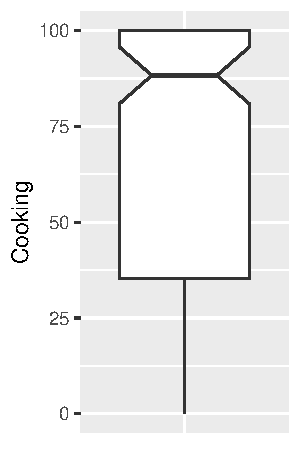
\includegraphics{b_files/figure-pdf/geomboxparam-1.pdf}

\section{geom\_bump}\label{bump}

\textbf{Package}

ggbump (Sjoberg 2020)

\textbf{Description}

Creates a smooth rank over time.

\textbf{Understandable aesthetics}

\emph{required aesthetics}

\texttt{x}, \texttt{y}

\emph{optional aesthetics}

\texttt{colour}, \texttt{alpha}, \texttt{size}

\textbf{See also}

\hyperref[line]{geom\_line}

\textbf{Example}

\begin{Shaded}
\begin{Highlighting}[]
\FunctionTok{library}\NormalTok{(ggbump)}
\NormalTok{a1 }\OtherTok{\textless{}{-}}\NormalTok{ worldbankdata }\SpecialCharTok{|\textgreater{}}
  \FunctionTok{filter}\NormalTok{(Country }\SpecialCharTok{==} \StringTok{"Afghanistan"}\NormalTok{) }\SpecialCharTok{|\textgreater{}}
  \FunctionTok{ggplot}\NormalTok{(}\FunctionTok{aes}\NormalTok{(}\AttributeTok{x =}\NormalTok{ Year, }\AttributeTok{y =}\NormalTok{ Electricity)) }\SpecialCharTok{+}
  \FunctionTok{geom\_bump}\NormalTok{() }\SpecialCharTok{+}
  \FunctionTok{ggtitle}\NormalTok{(}\StringTok{"a1: geom\_bump only"}\NormalTok{)}
\NormalTok{a2 }\OtherTok{\textless{}{-}}\NormalTok{ worldbankdata }\SpecialCharTok{|\textgreater{}}
  \FunctionTok{filter}\NormalTok{(Country }\SpecialCharTok{==} \StringTok{"Afghanistan"}\NormalTok{) }\SpecialCharTok{|\textgreater{}}
  \FunctionTok{ggplot}\NormalTok{(}\FunctionTok{aes}\NormalTok{(}\AttributeTok{x =}\NormalTok{ Year, }\AttributeTok{y =}\NormalTok{ Electricity)) }\SpecialCharTok{+}
  \FunctionTok{geom\_bump}\NormalTok{() }\SpecialCharTok{+}
  \FunctionTok{geom\_point}\NormalTok{() }\SpecialCharTok{+}
  \FunctionTok{ggtitle}\NormalTok{(}\StringTok{"a2: geom\_bump and geom\_point"}\NormalTok{)}
\NormalTok{a1 }\SpecialCharTok{|}\NormalTok{ a2}
\end{Highlighting}
\end{Shaded}

\includegraphics{b_files/figure-pdf/unnamed-chunk-13-1.pdf}

\part{C}

In this part of the book we will look at the geoms starts with letter
``c'' or ``C''.

\begin{longtable}[]{@{}lr@{}}
\toprule\noalign{}
geom & section \\
\midrule\noalign{}
\endhead
\bottomrule\noalign{}
\endlastfoot
geom\_col & 5.1 \\
geom\_col\_pattern & 5.2 \\
geom\_circle & 5.3 \\
\end{longtable}

\chapter{geom\_c}\label{sec-c}

\section{geom\_col}\label{geom_col}

\textbf{Package}

ggplot2 (Wickham 2016)

\textbf{Description}

Create bar charts

\textbf{Understandable aesthetics}

\emph{Required aesthetics}

\texttt{x}, \texttt{y}

\emph{Optional aesthetics}

\texttt{alpha}, \texttt{colour}, \texttt{fill}, \texttt{group},
\texttt{linetype}, \texttt{linewidth}

\textbf{See also}

\hyperref[bar]{geom\_bar}

\textbf{Example}

\begin{Shaded}
\begin{Highlighting}[]
\NormalTok{worldbankdata }\SpecialCharTok{|\textgreater{}}
  \FunctionTok{filter}\NormalTok{(Year }\SpecialCharTok{==} \DecValTok{2021}\NormalTok{) }\SpecialCharTok{|\textgreater{}}
  \FunctionTok{group\_by}\NormalTok{(Income) }\SpecialCharTok{|\textgreater{}}
  \FunctionTok{summarise}\NormalTok{(}\AttributeTok{n =} \FunctionTok{n}\NormalTok{()) }\SpecialCharTok{|\textgreater{}}
  \FunctionTok{ggplot}\NormalTok{(}\FunctionTok{aes}\NormalTok{(}\AttributeTok{x =}\NormalTok{ Income, }\AttributeTok{y =}\NormalTok{ n)) }\SpecialCharTok{+}   \FunctionTok{geom\_col}\NormalTok{()}
\end{Highlighting}
\end{Shaded}

\includegraphics{c_files/figure-pdf/unnamed-chunk-2-1.pdf}

\section{geom\_col\_pattern}\label{col_pattern}

\textbf{Package}

ggpattern (FC, Davis, and ggplot2 authors 2023)

\textbf{Description}

Fill columns with a pattern. User can map a variable for pattern or set
a pattern.

\textbf{Understandable aesthetics}

\emph{Required aesthetics}

\texttt{x}, \texttt{y}

\emph{Optional aesthetics}

\texttt{pattern}, \texttt{fill}, \texttt{colour}

\textbf{See also}

\hyperref[line]{geom\_line}, \hyperref[ribbon]{geom\_ribbon}

\textbf{Example}

\begin{Shaded}
\begin{Highlighting}[]
\NormalTok{worldbankdata }\SpecialCharTok{|\textgreater{}}
  \FunctionTok{filter}\NormalTok{(Year }\SpecialCharTok{==} \DecValTok{2021}\NormalTok{) }\SpecialCharTok{|\textgreater{}}
  \FunctionTok{group\_by}\NormalTok{(Income) }\SpecialCharTok{|\textgreater{}}
  \FunctionTok{summarise}\NormalTok{(}\AttributeTok{n =} \FunctionTok{n}\NormalTok{()) }\SpecialCharTok{|\textgreater{}}
  \FunctionTok{ggplot}\NormalTok{(}\FunctionTok{aes}\NormalTok{(}\AttributeTok{x =}\NormalTok{ Income, }\AttributeTok{y =}\NormalTok{ n)) }\SpecialCharTok{+}  
\NormalTok{  ggpattern}\SpecialCharTok{::}\FunctionTok{geom\_col\_pattern}\NormalTok{(}\FunctionTok{aes}\NormalTok{(}\AttributeTok{pattern =}\NormalTok{ n, }\AttributeTok{pattern\_angle=}\NormalTok{n),}
    \AttributeTok{colour  =} \StringTok{\textquotesingle{}black\textquotesingle{}}\NormalTok{, }\AttributeTok{fill=}\StringTok{"white"}\NormalTok{) }
\end{Highlighting}
\end{Shaded}

\includegraphics{c_files/figure-pdf/unnamed-chunk-3-1.pdf}

\section{geom\_count}\label{count}

\textbf{Package}

ggplo2t (Wickham 2016)

\textbf{Description}

Counts the observations at every point on the plot, and then maps the
count with the size of the point.

\textbf{Understandable aesthetics}

\emph{Required aesthetics}

\texttt{x}, \texttt{y}

\emph{Optional aesthetics}

\texttt{alpha}, \texttt{colour}, \texttt{fill}, \texttt{group},
\texttt{shape}, \texttt{size}, \texttt{stroke}

\textbf{See also}

\hyperref[point]{geom\_point}

\textbf{Example}

Here, both \texttt{geom\_point} and \texttt{geom\_count} are plotted to
see the difference.

\begin{Shaded}
\begin{Highlighting}[]
\NormalTok{a1 }\OtherTok{\textless{}{-}} \FunctionTok{ggplot}\NormalTok{(worldbankdata, }\FunctionTok{aes}\NormalTok{(}\AttributeTok{y =}\NormalTok{ Cooking, }\AttributeTok{x=}\NormalTok{Electricity)) }\SpecialCharTok{+} 
  \FunctionTok{geom\_point}\NormalTok{(}\AttributeTok{alpha =} \FloatTok{0.5}\NormalTok{) }\SpecialCharTok{+} 
  \FunctionTok{labs}\NormalTok{(}\AttributeTok{title =} \StringTok{"a1: geom\_point"}\NormalTok{) }\SpecialCharTok{+}
  \FunctionTok{theme}\NormalTok{(}\AttributeTok{aspect.ratio =} \DecValTok{1}\NormalTok{)}
\NormalTok{a2 }\OtherTok{\textless{}{-}} \FunctionTok{ggplot}\NormalTok{(worldbankdata, }\FunctionTok{aes}\NormalTok{(}\AttributeTok{y =}\NormalTok{ Cooking, }\AttributeTok{x=}\NormalTok{Electricity)) }\SpecialCharTok{+} 
  \FunctionTok{geom\_count}\NormalTok{() }\SpecialCharTok{+} 
  \FunctionTok{labs}\NormalTok{(}\AttributeTok{title =} \StringTok{"a2: geom\_count"}\NormalTok{) }\SpecialCharTok{+}
  \FunctionTok{theme}\NormalTok{(}\AttributeTok{aspect.ratio =} \DecValTok{1}\NormalTok{)}
\NormalTok{a1 }\SpecialCharTok{|}\NormalTok{ a2}
\end{Highlighting}
\end{Shaded}

\includegraphics{c_files/figure-pdf/unnamed-chunk-4-1.pdf}

\section{geom\_circle}\label{circle}

\textbf{Package}

ggforce (Pedersen 2022)

\textbf{Description}

Draw circles based on a center point and a radius.

\textbf{Understandable aesthetics}

\emph{required aesthetics}

\texttt{x0} - starting coordinate of x-axis , \texttt{y0} - starting
coordinate of x-axis, \texttt{r} - radius

\emph{optional aesthetics}

\texttt{color}, \texttt{fill}, \texttt{linewidth}, \texttt{linetype},
\texttt{alpha}, \texttt{lineend}

\textbf{See also}

\hyperref[mark_circle]{geom\_mark\_circle}

\textbf{Example}

\begin{Shaded}
\begin{Highlighting}[]
\NormalTok{worldbankdata }\SpecialCharTok{|\textgreater{}}
  \FunctionTok{filter}\NormalTok{(Year }\SpecialCharTok{==} \DecValTok{2021}\NormalTok{) }\SpecialCharTok{|\textgreater{}}
\FunctionTok{ggplot}\NormalTok{(}\FunctionTok{aes}\NormalTok{(}\AttributeTok{y =}\NormalTok{ Cooking, }\AttributeTok{x=}\NormalTok{Electricity, }\AttributeTok{col=}\NormalTok{Income)) }\SpecialCharTok{+} 
  \FunctionTok{geom\_point}\NormalTok{() }\SpecialCharTok{+} 
  \FunctionTok{scale\_color\_brewer}\NormalTok{(}\AttributeTok{palette =} \StringTok{"Dark2"}\NormalTok{) }\SpecialCharTok{+}
\NormalTok{  ggforce}\SpecialCharTok{::}\FunctionTok{geom\_circle}\NormalTok{(}\FunctionTok{aes}\NormalTok{(}\AttributeTok{x0 =} \DecValTok{26}\NormalTok{, }\AttributeTok{y0 =} \DecValTok{5}\NormalTok{, }\AttributeTok{r =} \DecValTok{20}\NormalTok{),}
              \AttributeTok{inherit.aes =} \ConstantTok{FALSE}\NormalTok{) }\SpecialCharTok{+} 
    \FunctionTok{theme}\NormalTok{(}\AttributeTok{aspect.ratio =} \DecValTok{1}\NormalTok{)}
\end{Highlighting}
\end{Shaded}

\includegraphics{c_files/figure-pdf/unnamed-chunk-5-1.pdf}

\section{geom\_contour}\label{contour}

\textbf{Package}

ggplot2 (Wickham 2016)

\textbf{Description}

Create contour plots.

\textbf{Understandable aesthetics}

\emph{Required aesthetics}

\texttt{x}, \texttt{y}

\emph{Optional aesthetics}

\texttt{alpha}, \texttt{colour}, \texttt{fill} , \texttt{group},
\texttt{linetype}, \texttt{linewidth}, \texttt{subgroup}

\textbf{See also}

\hyperref[contour_filled]{geom\_contour\_filled},
\hyperref[tile]{geom\_tile}, \hyperref[density_2d]{geom\_density\_2d}

\textbf{Example}

\begin{Shaded}
\begin{Highlighting}[]
\NormalTok{mean }\OtherTok{\textless{}{-}} \FunctionTok{c}\NormalTok{(}\FloatTok{0.5}\NormalTok{, }\SpecialCharTok{{-}}\FloatTok{0.5}\NormalTok{)}
\NormalTok{sigma }\OtherTok{\textless{}{-}} \FunctionTok{matrix}\NormalTok{(}\FunctionTok{c}\NormalTok{(}\DecValTok{1}\NormalTok{, }\FloatTok{0.5}\NormalTok{, }\FloatTok{0.5}\NormalTok{, }\DecValTok{1}\NormalTok{), }\AttributeTok{nrow=}\DecValTok{2}\NormalTok{)}
\NormalTok{data.grid }\OtherTok{\textless{}{-}} \FunctionTok{expand.grid}\NormalTok{(}\AttributeTok{x=}\FunctionTok{seq}\NormalTok{(}\SpecialCharTok{{-}}\DecValTok{3}\NormalTok{, }\DecValTok{3}\NormalTok{, }\AttributeTok{length.out=}\DecValTok{200}\NormalTok{),}
                         \AttributeTok{y=}\FunctionTok{seq}\NormalTok{(}\SpecialCharTok{{-}}\DecValTok{3}\NormalTok{, }\DecValTok{3}\NormalTok{, }\AttributeTok{length.out=}\DecValTok{200}\NormalTok{))}
\NormalTok{df }\OtherTok{\textless{}{-}} \FunctionTok{cbind}\NormalTok{(data.grid, }\AttributeTok{prob =}\NormalTok{ mvtnorm}\SpecialCharTok{::}\FunctionTok{dmvnorm}\NormalTok{(data.grid, }\AttributeTok{mean=}\NormalTok{mean, }\AttributeTok{sigma=}\NormalTok{sigma))}
\FunctionTok{ggplot}\NormalTok{(df, }\FunctionTok{aes}\NormalTok{(}\AttributeTok{x=}\NormalTok{x, }\AttributeTok{y=}\NormalTok{y, }\AttributeTok{z=}\NormalTok{prob)) }\SpecialCharTok{+} 
  \FunctionTok{geom\_contour}\NormalTok{() }\SpecialCharTok{+} 
  \FunctionTok{theme}\NormalTok{(}\AttributeTok{aspect.ratio =} \DecValTok{1}\NormalTok{)}
\end{Highlighting}
\end{Shaded}

\includegraphics{c_files/figure-pdf/unnamed-chunk-6-1.pdf}

\section{geom\_contour\_filled}\label{contour_filled}

\textbf{Package}

ggplot2 (Wickham 2016)

\textbf{Description}

Create contour plots

\textbf{Understandable aesthetics}

\texttt{x}, \texttt{y}, \texttt{alpha}, \texttt{colour},
\texttt{linetype}, \texttt{linewidth}, \texttt{group}, \texttt{weight}

\textbf{See also}

\hyperref[contour]{geom\_contour}, \hyperref[tile]{geom\_tile},
\hyperref[density_2d]{geom\_density\_2d}

\textbf{Example}

\begin{Shaded}
\begin{Highlighting}[]
\NormalTok{mean }\OtherTok{\textless{}{-}} \FunctionTok{c}\NormalTok{(}\FloatTok{0.5}\NormalTok{, }\SpecialCharTok{{-}}\FloatTok{0.5}\NormalTok{)}
\NormalTok{sigma }\OtherTok{\textless{}{-}} \FunctionTok{matrix}\NormalTok{(}\FunctionTok{c}\NormalTok{(}\DecValTok{1}\NormalTok{, }\FloatTok{0.5}\NormalTok{, }\FloatTok{0.5}\NormalTok{, }\DecValTok{1}\NormalTok{), }\AttributeTok{nrow=}\DecValTok{2}\NormalTok{)}
\NormalTok{data.grid }\OtherTok{\textless{}{-}} \FunctionTok{expand.grid}\NormalTok{(}\AttributeTok{x=}\FunctionTok{seq}\NormalTok{(}\SpecialCharTok{{-}}\DecValTok{3}\NormalTok{, }\DecValTok{3}\NormalTok{, }\AttributeTok{length.out=}\DecValTok{200}\NormalTok{),}
                         \AttributeTok{y=}\FunctionTok{seq}\NormalTok{(}\SpecialCharTok{{-}}\DecValTok{3}\NormalTok{, }\DecValTok{3}\NormalTok{, }\AttributeTok{length.out=}\DecValTok{200}\NormalTok{))}
\NormalTok{df }\OtherTok{\textless{}{-}} \FunctionTok{cbind}\NormalTok{(data.grid, }\AttributeTok{prob =}\NormalTok{ mvtnorm}\SpecialCharTok{::}\FunctionTok{dmvnorm}\NormalTok{(data.grid, }\AttributeTok{mean=}\NormalTok{mean, }\AttributeTok{sigma=}\NormalTok{sigma))}
\FunctionTok{ggplot}\NormalTok{(df, }\FunctionTok{aes}\NormalTok{(}\AttributeTok{x=}\NormalTok{x, }\AttributeTok{y=}\NormalTok{y, }\AttributeTok{z=}\NormalTok{prob)) }\SpecialCharTok{+} 
  \FunctionTok{geom\_contour\_filled}\NormalTok{() }\SpecialCharTok{+} 
  \FunctionTok{theme}\NormalTok{(}\AttributeTok{aspect.ratio =} \DecValTok{1}\NormalTok{)}
\end{Highlighting}
\end{Shaded}

\includegraphics{c_files/figure-pdf/unnamed-chunk-7-1.pdf}

\section{geom\_curve}\label{curve}

\textbf{Package}

ggplot2 (Wickham 2016)

\textbf{Description}

\texttt{geom\_segment()} draws a straight line between between two
points. geom\_curve draws a curved line.

\textbf{Understandable aesthetics}

\emph{required aesthetics}

\texttt{x}, \texttt{y}

\emph{optional aesthetics}

\texttt{alpha}, \texttt{colour}, \texttt{linetype}, \texttt{linewidth},
\texttt{group}

\textbf{The statistical transformation to use on the data for this
layer}

\texttt{identity}

\textbf{See also}

\hyperref[segment]{geom\_segment}

\textbf{Examples}

\begin{Shaded}
\begin{Highlighting}[]
\NormalTok{df }\OtherTok{\textless{}{-}} \FunctionTok{data.frame}\NormalTok{(}\AttributeTok{x1 =} \DecValTok{0}\NormalTok{, }\AttributeTok{x2 =} \DecValTok{100}\NormalTok{, }\AttributeTok{y1 =} \DecValTok{0}\NormalTok{, }\AttributeTok{y2 =} \DecValTok{100}\NormalTok{)}
\FunctionTok{ggplot}\NormalTok{(df) }\SpecialCharTok{+} 
  \FunctionTok{geom\_curve}\NormalTok{(}\FunctionTok{aes}\NormalTok{(}\AttributeTok{x =}\NormalTok{ x1, }\AttributeTok{y =}\NormalTok{ y1, }\AttributeTok{xend =}\NormalTok{ x2, }\AttributeTok{yend =}\NormalTok{ y2))}
\end{Highlighting}
\end{Shaded}

\includegraphics{c_files/figure-pdf/unnamed-chunk-8-1.pdf}

\begin{Shaded}
\begin{Highlighting}[]
\NormalTok{df }\OtherTok{\textless{}{-}} \FunctionTok{data.frame}\NormalTok{(}\AttributeTok{x2 =} \FunctionTok{c}\NormalTok{( }\DecValTok{3}\NormalTok{, }\DecValTok{4}\NormalTok{, }\DecValTok{4}\NormalTok{, }\DecValTok{3}\NormalTok{, }\SpecialCharTok{{-}}\DecValTok{3}\NormalTok{, }\SpecialCharTok{{-}}\DecValTok{4}\NormalTok{, }\SpecialCharTok{{-}}\DecValTok{4}\NormalTok{, }\SpecialCharTok{{-}}\DecValTok{3}\NormalTok{),}
                 \AttributeTok{y2 =} \FunctionTok{c}\NormalTok{( }\DecValTok{4}\NormalTok{, }\DecValTok{3}\NormalTok{, }\SpecialCharTok{{-}}\DecValTok{3}\NormalTok{, }\SpecialCharTok{{-}}\DecValTok{4}\NormalTok{, }\SpecialCharTok{{-}}\DecValTok{4}\NormalTok{, }\SpecialCharTok{{-}}\DecValTok{3}\NormalTok{, }\DecValTok{3}\NormalTok{, }\DecValTok{3}\NormalTok{),}
                 \AttributeTok{x1 =} \FunctionTok{rep}\NormalTok{(}\DecValTok{0}\NormalTok{, }\DecValTok{8}\NormalTok{),}
                 \AttributeTok{y1 =} \FunctionTok{rep}\NormalTok{(}\DecValTok{0}\NormalTok{, }\DecValTok{8}\NormalTok{))}

\FunctionTok{ggplot}\NormalTok{(df) }\SpecialCharTok{+} 
  \FunctionTok{geom\_curve}\NormalTok{(}\FunctionTok{aes}\NormalTok{(}\AttributeTok{x =}\NormalTok{ x1, }\AttributeTok{y =}\NormalTok{ y1, }\AttributeTok{xend =}\NormalTok{ x2, }\AttributeTok{yend =}\NormalTok{ y2),}
             \AttributeTok{curvature =} \FloatTok{0.75}\NormalTok{, }\AttributeTok{angle =} \SpecialCharTok{{-}}\DecValTok{45}\NormalTok{,}
             \AttributeTok{arrow =} \FunctionTok{arrow}\NormalTok{(}\AttributeTok{length =} \FunctionTok{unit}\NormalTok{(}\FloatTok{0.25}\NormalTok{,}\StringTok{"cm"}\NormalTok{))) }\SpecialCharTok{+} 
  \FunctionTok{coord\_equal}\NormalTok{() }\SpecialCharTok{+}
  \FunctionTok{xlim}\NormalTok{(}\SpecialCharTok{{-}}\DecValTok{5}\NormalTok{, }\DecValTok{5}\NormalTok{) }\SpecialCharTok{+} \FunctionTok{ylim}\NormalTok{(}\SpecialCharTok{{-}}\DecValTok{5}\NormalTok{, }\DecValTok{5}\NormalTok{)}
\end{Highlighting}
\end{Shaded}

\includegraphics{c_files/figure-pdf/unnamed-chunk-9-1.pdf}

\section{geom\_crossbar}\label{crossbar}

\textbf{Package}

ggplot2 (Wickham 2016)

\textbf{Description}

Plot a vertical interval defined by y, ymin and ymax or x, xmin and
xmax.

\textbf{Understandable aesthetics}

\emph{required aesthetics}

\texttt{x} or \texttt{y}

\texttt{xmin} or \texttt{ymin}

\texttt{xmax} or \texttt{ymax}

\emph{optional aesthetics}

\texttt{alpha}, \texttt{colour}, \texttt{linetype}, \texttt{linewidth},
\texttt{group}

\textbf{See also}

\hyperref[segment]{geom\_segment}

\textbf{Examples}

\emph{Example 1}

\begin{Shaded}
\begin{Highlighting}[]
\NormalTok{summarydf }\OtherTok{\textless{}{-}}\NormalTok{ worldbankdata }\SpecialCharTok{|\textgreater{}}
  \FunctionTok{drop\_na}\NormalTok{() }\SpecialCharTok{|\textgreater{}}
  \FunctionTok{select}\NormalTok{(Electricity, Income) }\SpecialCharTok{|\textgreater{}}
  \FunctionTok{group\_by}\NormalTok{(Income) }\SpecialCharTok{|\textgreater{}}
  \FunctionTok{reframe}\NormalTok{(}\AttributeTok{qs =} \FunctionTok{quantile}\NormalTok{(Electricity, }\FunctionTok{c}\NormalTok{(}\FloatTok{0.25}\NormalTok{, }\FloatTok{0.5}\NormalTok{ ,}\FloatTok{0.75}\NormalTok{))) }\SpecialCharTok{|\textgreater{}}
  \FunctionTok{mutate}\NormalTok{(}\AttributeTok{q=}\FunctionTok{rep}\NormalTok{(}\FunctionTok{c}\NormalTok{(}\StringTok{"Q1"}\NormalTok{, }\StringTok{"Q2"}\NormalTok{, }\StringTok{"Q3"}\NormalTok{), }\DecValTok{4}\NormalTok{)) }\SpecialCharTok{|\textgreater{}}
  \FunctionTok{pivot\_wider}\NormalTok{(}\AttributeTok{names\_from =}\NormalTok{ q,}
              \AttributeTok{values\_from =}\NormalTok{ qs)}
\NormalTok{summarydf}
\end{Highlighting}
\end{Shaded}

\begin{verbatim}
# A tibble: 4 x 4
  Income    Q1    Q2    Q3
  <fct>  <dbl> <dbl> <dbl>
1 L       16.6  32.2  50.7
2 LM      62.0  86.7  97.7
3 UM      95.9  99.5 100. 
4 H      100   100   100  
\end{verbatim}

\begin{Shaded}
\begin{Highlighting}[]
\FunctionTok{ggplot}\NormalTok{(summarydf, }\FunctionTok{aes}\NormalTok{(}\AttributeTok{x=}\NormalTok{Income, }\AttributeTok{ymin =}\NormalTok{ Q1, }\AttributeTok{y=}\NormalTok{Q2, }\AttributeTok{ymax =}\NormalTok{ Q3)) }\SpecialCharTok{+} 
  \FunctionTok{geom\_crossbar}\NormalTok{(}\AttributeTok{size=}\DecValTok{1}\NormalTok{,}\AttributeTok{col=}\StringTok{"red"}\NormalTok{, }\AttributeTok{width =}\NormalTok{ .}\DecValTok{5}\NormalTok{)}
\end{Highlighting}
\end{Shaded}

\includegraphics{c_files/figure-pdf/unnamed-chunk-10-1.pdf}

\emph{Example 2}

\begin{Shaded}
\begin{Highlighting}[]
\NormalTok{summary\_stats }\OtherTok{\textless{}{-}}\NormalTok{ worldbankdata }\SpecialCharTok{|\textgreater{}}
  \FunctionTok{drop\_na}\NormalTok{() }\SpecialCharTok{|\textgreater{}}
  \FunctionTok{select}\NormalTok{(Electricity, Income) }\SpecialCharTok{|\textgreater{}}
  \FunctionTok{group\_by}\NormalTok{(Income) }\SpecialCharTok{|\textgreater{}}
  \FunctionTok{reframe}\NormalTok{(}\AttributeTok{mean =} \FunctionTok{mean}\NormalTok{(Electricity),}
          \AttributeTok{sd =} \FunctionTok{sd}\NormalTok{(Electricity)) }
\FunctionTok{ggplot}\NormalTok{(summary\_stats, }\FunctionTok{aes}\NormalTok{(}\AttributeTok{x =}\NormalTok{ Income, }\AttributeTok{y =}\NormalTok{ mean, }\AttributeTok{ymin =}\NormalTok{ mean }\SpecialCharTok{{-}}\NormalTok{ sd, }\AttributeTok{ymax =}\NormalTok{ mean }\SpecialCharTok{+}\NormalTok{ sd)) }\SpecialCharTok{+}
  \FunctionTok{geom\_crossbar}\NormalTok{(}\AttributeTok{width =} \FloatTok{0.5}\NormalTok{, }\AttributeTok{fatten =} \DecValTok{2}\NormalTok{) }
\end{Highlighting}
\end{Shaded}

\includegraphics{c_files/figure-pdf/unnamed-chunk-11-1.pdf}

\part{D}

In this part of the book we will look at the geoms starts with letter
``d'' or ``D''.

\begin{longtable}[]{@{}lr@{}}
\toprule\noalign{}
geom & section \\
\midrule\noalign{}
\endhead
\bottomrule\noalign{}
\endlastfoot
geom\_d & 6.1 \\
\end{longtable}

\chapter{geom\_d}\label{sec-d}

\section{geom\_density}\label{density}

\textbf{Package}

ggplot2 (Wickham 2016)

\textbf{Description}

Computes and draws kernel density estimation.

\textbf{Understandable aesthetics}

\emph{required aesthetics}

\texttt{x}, \texttt{y}

\emph{optional aesthetics}

\texttt{alpha}, \texttt{colour}, \texttt{fill}, \texttt{group},
\texttt{linetype}, \texttt{linewidth}, \texttt{weight}

\textbf{See also}

\hyperref[hist]{geom\_histogram}

\textbf{Example}

\begin{Shaded}
\begin{Highlighting}[]
\NormalTok{worldbankdata }\SpecialCharTok{|\textgreater{}}
  \FunctionTok{ggplot}\NormalTok{(}\FunctionTok{aes}\NormalTok{(}\AttributeTok{x =}\NormalTok{ Electricity)) }\SpecialCharTok{+}   \FunctionTok{geom\_density}\NormalTok{()}
\end{Highlighting}
\end{Shaded}

\includegraphics{d_files/figure-pdf/unnamed-chunk-2-1.pdf}

\section{geom\_density\_line}\label{density_line}

\textbf{Package}

ggridges (Wilke 2023)

\textbf{Description}

Draws a density plot same as geom\_density. The difference is that the
geom draws a ridgeline (line with filled area underneath).

\textbf{Understandable aesthetics}

\emph{required aesthetics}

\texttt{x}

\texttt{y}

\emph{optional aesthetics}

\texttt{alpha}, \texttt{colour}, \texttt{fill}, \texttt{group},
\texttt{linetype}, \texttt{linewidth}, \texttt{weight}

\textbf{See also}

\hyperref[density]{geom\_density}

\textbf{Example}

\begin{Shaded}
\begin{Highlighting}[]
\FunctionTok{library}\NormalTok{(ggridges)}
\NormalTok{worldbankdata }\SpecialCharTok{|\textgreater{}}
  \FunctionTok{ggplot}\NormalTok{(}\FunctionTok{aes}\NormalTok{(}\AttributeTok{x =}\NormalTok{ Electricity)) }\SpecialCharTok{+}   
  \FunctionTok{geom\_density\_line}\NormalTok{()}
\end{Highlighting}
\end{Shaded}

\includegraphics{d_files/figure-pdf/unnamed-chunk-3-1.pdf}

\section{geom\_density\_2d}\label{density_2d}

\textbf{Package}

ggplot2 (Wickham 2016)

\textbf{Description}

Computes a 2D kernel density estimation using \texttt{MASS::kde2d()} and
display the results with contours.

\textbf{Understandable aesthetics}

\texttt{stat\_density}

\emph{required aesthetics}

\texttt{x}

\texttt{y}

\emph{optional aesthetics}

\texttt{alpha}, \texttt{colour}, \texttt{group}, \texttt{linetype},
\texttt{linewidth}

\textbf{See also}

\hyperref[hist]{geom\_histofram}

\textbf{Example}

\begin{Shaded}
\begin{Highlighting}[]
\NormalTok{a1 }\OtherTok{\textless{}{-}}\NormalTok{ worldbankdata }\SpecialCharTok{|\textgreater{}}
  \FunctionTok{ggplot}\NormalTok{(}\FunctionTok{aes}\NormalTok{(}\AttributeTok{y =}\NormalTok{ Cooking, }\AttributeTok{x=}\NormalTok{Electricity)) }\SpecialCharTok{+}   
  \FunctionTok{geom\_density\_2d}\NormalTok{() }\SpecialCharTok{+}
  \FunctionTok{xlim}\NormalTok{(}\DecValTok{0}\NormalTok{, }\DecValTok{100}\NormalTok{) }\SpecialCharTok{+}
  \FunctionTok{ylim}\NormalTok{(}\DecValTok{0}\NormalTok{, }\DecValTok{100}\NormalTok{) }\SpecialCharTok{+}
  \FunctionTok{theme}\NormalTok{(}\AttributeTok{aspect.ratio =} \DecValTok{1}\NormalTok{) }\SpecialCharTok{+} 
  \FunctionTok{labs}\NormalTok{(}\AttributeTok{title =} \StringTok{"a1: geom\_density\_2d only"}\NormalTok{)}
\NormalTok{a2 }\OtherTok{\textless{}{-}}\NormalTok{ worldbankdata }\SpecialCharTok{|\textgreater{}}
  \FunctionTok{ggplot}\NormalTok{(}\FunctionTok{aes}\NormalTok{(}\AttributeTok{y =}\NormalTok{ Cooking, }\AttributeTok{x=}\NormalTok{Electricity)) }\SpecialCharTok{+}   
  \FunctionTok{geom\_point}\NormalTok{() }\SpecialCharTok{+}
  \FunctionTok{geom\_density\_2d}\NormalTok{() }\SpecialCharTok{+}
  \FunctionTok{theme}\NormalTok{(}\AttributeTok{aspect.ratio =} \DecValTok{1}\NormalTok{) }\SpecialCharTok{+} 
  \FunctionTok{labs}\NormalTok{(}\AttributeTok{title =} \StringTok{"a2: geom\_point and }\SpecialCharTok{\textbackslash{}n}\StringTok{ geom\_density\_2d"}\NormalTok{) }
  
\NormalTok{a1}\SpecialCharTok{|}\NormalTok{a2}
\end{Highlighting}
\end{Shaded}

\includegraphics{d_files/figure-pdf/unnamed-chunk-4-1.pdf}

\section{geom\_density\_2d\_filled}\label{density_2d_filled}

\textbf{Package}

ggplot2 (Wickham 2016)

\textbf{Description}

Computes a 2D kernel density estimation using \texttt{MASS::kde2d()} and
display the results with filled contour bands.

\textbf{Understandable aesthetics}

\emph{required aesthetics}

\texttt{x}

\texttt{y}

\emph{optional aesthetics}

\texttt{alpha}, \texttt{colour}, \texttt{group}, \texttt{linetype},
\texttt{linewidth}, \texttt{subgroup}

\textbf{See also}

\hyperref[hist]{geom\_histogram}

\textbf{Example}

\begin{Shaded}
\begin{Highlighting}[]
\NormalTok{a1 }\OtherTok{\textless{}{-}}\NormalTok{ worldbankdata }\SpecialCharTok{|\textgreater{}}
  \FunctionTok{filter}\NormalTok{(Year }\SpecialCharTok{==} \StringTok{"2021"}\NormalTok{) }\SpecialCharTok{|\textgreater{}}
  \FunctionTok{ggplot}\NormalTok{(}\FunctionTok{aes}\NormalTok{(}\AttributeTok{y =}\NormalTok{ Cooking, }\AttributeTok{x=}\NormalTok{Electricity)) }\SpecialCharTok{+}   
  \FunctionTok{geom\_density\_2d\_filled}\NormalTok{() }\SpecialCharTok{+} 
  \FunctionTok{labs}\NormalTok{(}\AttributeTok{title =} \StringTok{"a1: geom\_density\_2d\_filled only"}\NormalTok{) }\SpecialCharTok{+} 
  \FunctionTok{theme}\NormalTok{( }\AttributeTok{aspect.ratio =} \DecValTok{1}\NormalTok{)}
\NormalTok{a2 }\OtherTok{\textless{}{-}}\NormalTok{ worldbankdata }\SpecialCharTok{|\textgreater{}}
  \FunctionTok{filter}\NormalTok{(Year }\SpecialCharTok{==} \StringTok{"2020"}\NormalTok{) }\SpecialCharTok{|\textgreater{}}
  \FunctionTok{ggplot}\NormalTok{(}\FunctionTok{aes}\NormalTok{(}\AttributeTok{y =}\NormalTok{ Cooking, }\AttributeTok{x=}\NormalTok{Electricity)) }\SpecialCharTok{+}   
  \FunctionTok{geom\_density\_2d\_filled}\NormalTok{(}\AttributeTok{alpha =} \FloatTok{0.5}\NormalTok{) }\SpecialCharTok{+} 
    \FunctionTok{geom\_point}\NormalTok{() }\SpecialCharTok{+} 
  \FunctionTok{labs}\NormalTok{(}\AttributeTok{title =} \StringTok{"a2: geom\_point and }\SpecialCharTok{\textbackslash{}n}\StringTok{ geom\_density\_2d\_filled"}\NormalTok{) }\SpecialCharTok{+} 
  \FunctionTok{theme}\NormalTok{( }\AttributeTok{aspect.ratio =} \DecValTok{1}\NormalTok{)}
\NormalTok{a3 }\OtherTok{\textless{}{-}}\NormalTok{ worldbankdata }\SpecialCharTok{|\textgreater{}}
  \FunctionTok{filter}\NormalTok{(Year }\SpecialCharTok{==} \StringTok{"2020"}\NormalTok{) }\SpecialCharTok{|\textgreater{}}
  \FunctionTok{ggplot}\NormalTok{(}\FunctionTok{aes}\NormalTok{(}\AttributeTok{y =}\NormalTok{ Cooking, }\AttributeTok{x=}\NormalTok{Electricity)) }\SpecialCharTok{+}   
  \FunctionTok{geom\_point}\NormalTok{(}\AttributeTok{alpha=}\FloatTok{0.5}\NormalTok{) }\SpecialCharTok{+} 
  \FunctionTok{labs}\NormalTok{(}\AttributeTok{title =} \StringTok{"a3: geom\_point"}\NormalTok{) }\SpecialCharTok{+} 
  \FunctionTok{theme}\NormalTok{(}\AttributeTok{aspect.ratio =} \DecValTok{1}\NormalTok{)}
\NormalTok{a1 }\SpecialCharTok{/}\NormalTok{ a2 }\SpecialCharTok{/}\NormalTok{ a3}
\end{Highlighting}
\end{Shaded}

\includegraphics{d_files/figure-pdf/unnamed-chunk-5-1.pdf}

\section{geom\_density\_ridges}\label{density_ridges}

\textbf{Package}

ggridges (Wilke 2023)

\textbf{Description}

Arranges multiple density plots in a staggered fashion.

\textbf{Understandable aesthetics}

\emph{required aesthetics}

\texttt{x}, \texttt{y}

\emph{optional aesthetics}

\texttt{colour}, \texttt{fill}, \texttt{group}, \texttt{height},
\texttt{alpha}, \texttt{linetype}, \texttt{linewidth}, \texttt{scale},
\texttt{rel\_min\_height}

\textbf{See also}

\hyperref[density_ridges_gradient]{geom\_density\_ridges\_gradient}

\textbf{Example}

\begin{Shaded}
\begin{Highlighting}[]
\FunctionTok{library}\NormalTok{(ggridges)}
\NormalTok{ worldbankdata }\SpecialCharTok{|\textgreater{}}
  \FunctionTok{ggplot}\NormalTok{(}\FunctionTok{aes}\NormalTok{(}\AttributeTok{y =}\NormalTok{ Income, }\AttributeTok{x=}\NormalTok{Electricity)) }\SpecialCharTok{+}   
  \FunctionTok{geom\_density\_ridges}\NormalTok{() }
\end{Highlighting}
\end{Shaded}

\includegraphics{d_files/figure-pdf/unnamed-chunk-6-1.pdf}

\section{geom\_density\_ridges\_gradient}\label{density_ridges_gradient}

\textbf{Package}

ggridges (Wilke 2023)

\textbf{Description}

Arranges multiple density plots in a staggered fashion.

\textbf{Understandable aesthetics}

\emph{required aesthetics}

\texttt{x}, \texttt{y}

\emph{optional aesthetics}

\texttt{colour}, \texttt{fill}, \texttt{group}, \texttt{height},
\texttt{alpha}, \texttt{linetype}, \texttt{linewidth}, \texttt{scale},
\texttt{rel\_min\_height}

\textbf{See also}

\hyperref[density_ridges]{geom\_density\_ridges}

\textbf{Example}

\begin{Shaded}
\begin{Highlighting}[]
\FunctionTok{library}\NormalTok{(ggridges)}
\NormalTok{ worldbankdata }\SpecialCharTok{|\textgreater{}}
  \FunctionTok{ggplot}\NormalTok{(}\FunctionTok{aes}\NormalTok{(}\AttributeTok{y =}\NormalTok{ Income, }\AttributeTok{x=}\NormalTok{Electricity, }\AttributeTok{fill=}\FunctionTok{stat}\NormalTok{(x))) }\SpecialCharTok{+}   
  \FunctionTok{geom\_density\_ridges\_gradient}\NormalTok{() }\SpecialCharTok{+}
  \FunctionTok{scale\_fill\_viridis\_c}\NormalTok{()}
\end{Highlighting}
\end{Shaded}

\includegraphics{d_files/figure-pdf/unnamed-chunk-7-1.pdf}

\section{geom\_dl}\label{dl}

\textbf{Package}

directlabels (Hocking 2023)

\textbf{Description}

Display direct labels on the plot.

\textbf{Understandable aesthetics}

\texttt{layer}

\textbf{See also}

\hyperref[text]{geom\_text}

\textbf{Example}

\begin{Shaded}
\begin{Highlighting}[]
\FunctionTok{library}\NormalTok{(directlabels)}
\NormalTok{a1 }\OtherTok{\textless{}{-}}\NormalTok{ worldbankdata }\SpecialCharTok{|\textgreater{}}
  \FunctionTok{ggplot}\NormalTok{(}\FunctionTok{aes}\NormalTok{(}\AttributeTok{y =}\NormalTok{ Cooking, }\AttributeTok{x=}\NormalTok{Electricity)) }\SpecialCharTok{+}   
  \FunctionTok{geom\_point}\NormalTok{(}\FunctionTok{aes}\NormalTok{(}\AttributeTok{col=}\NormalTok{Income)) }\SpecialCharTok{+}
  \FunctionTok{theme}\NormalTok{(}\AttributeTok{aspect.ratio =} \DecValTok{1}\NormalTok{) }\SpecialCharTok{+}
  \FunctionTok{scale\_color\_brewer}\NormalTok{(}\AttributeTok{palette =} \StringTok{"Set1"}\NormalTok{)}
\NormalTok{a1 }\SpecialCharTok{+}
  \FunctionTok{geom\_dl}\NormalTok{(}\FunctionTok{aes}\NormalTok{(}\AttributeTok{label=}\NormalTok{Income), }\AttributeTok{method=}\StringTok{"smart.grid"}\NormalTok{)}\SpecialCharTok{+}
  \FunctionTok{scale\_shape\_manual}\NormalTok{(}\AttributeTok{values=}\FunctionTok{c}\NormalTok{(}\AttributeTok{H =} \DecValTok{1}\NormalTok{, }
                              \AttributeTok{UM =} \DecValTok{6}\NormalTok{,}
                              \AttributeTok{L =} \DecValTok{3}\NormalTok{,}
                              \AttributeTok{LM =} \DecValTok{2}\NormalTok{),}
                     \AttributeTok{guide=}\StringTok{"none"}\NormalTok{)}
\end{Highlighting}
\end{Shaded}

\includegraphics{d_files/figure-pdf/unnamed-chunk-8-1.pdf}

\section{geom\_dotplot}\label{dotplot}

\textbf{Package}

ggplot2 (Wickham 2016)

\textbf{Description}

Create dotplot.

\subsection{Understandable aesthetics}\label{understandable-aesthetics}

\emph{required aesthetics}

\texttt{x} or \texttt{y}

\emph{optional aesthetics}

\texttt{alpha}, \texttt{colour}, \texttt{fill} , \texttt{group},
\texttt{linetype}, \texttt{stroke}

\textbf{See also}

\hyperref[hist]{geom\_histogram}

\textbf{Example}

\begin{Shaded}
\begin{Highlighting}[]
\NormalTok{worldbankdata }\SpecialCharTok{|\textgreater{}}
  \FunctionTok{ggplot}\NormalTok{(}\FunctionTok{aes}\NormalTok{(}\AttributeTok{x=}\NormalTok{Cooking)) }\SpecialCharTok{+}   
  \FunctionTok{geom\_dotplot}\NormalTok{(}\AttributeTok{binwidth =} \DecValTok{1}\NormalTok{) }\SpecialCharTok{+} 
  \FunctionTok{theme}\NormalTok{(}\AttributeTok{legend.position=}\StringTok{"none"}\NormalTok{, }\AttributeTok{aspect.ratio =} \DecValTok{1}\NormalTok{)}
\end{Highlighting}
\end{Shaded}

\includegraphics{d_files/figure-pdf/unnamed-chunk-9-1.pdf}

\section{geom\_delaunay\_tile}\label{delaunay_tile}

\textbf{Package}

ggforce (Pedersen 2022)

\textbf{Description}

Display voronoi tesselation and delaunay triangulation.

\textbf{Understandable aesthetics}

\emph{required aesthetics}

\texttt{x} or \texttt{y}

\emph{optional aesthetics}

\texttt{alpha}, \texttt{colour}, \texttt{fill} , \texttt{linetype},
\texttt{size}

\textbf{See also}

\hyperref[delaunay_segment]{geom\_delaunay\_segment}

\textbf{Example}

\begin{Shaded}
\begin{Highlighting}[]
\FunctionTok{library}\NormalTok{(ggforce)}
\FunctionTok{library}\NormalTok{(deldir) }\CommentTok{\#to calculate delaunay triangulation}
\NormalTok{a1 }\OtherTok{\textless{}{-}}\NormalTok{ worldbankdata }\SpecialCharTok{|\textgreater{}}
  \FunctionTok{filter}\NormalTok{(Income }\SpecialCharTok{==} \StringTok{"L"}\NormalTok{) }\SpecialCharTok{|\textgreater{}}
  \FunctionTok{ggplot}\NormalTok{(}\FunctionTok{aes}\NormalTok{(}\AttributeTok{x=}\NormalTok{Cooking, }\AttributeTok{y=}\NormalTok{Electricity)) }\SpecialCharTok{+}   
  \FunctionTok{geom\_delaunay\_tile}\NormalTok{(}\AttributeTok{alpha=}\FloatTok{0.5}\NormalTok{) }\SpecialCharTok{+} 
  \FunctionTok{labs}\NormalTok{(}\AttributeTok{title =} \StringTok{"a1: geom\_delaunay\_tile only"}\NormalTok{) }\SpecialCharTok{+}
  \FunctionTok{theme}\NormalTok{(}\AttributeTok{aspect.ratio =} \DecValTok{1}\NormalTok{)}

\NormalTok{a2 }\OtherTok{\textless{}{-}}\NormalTok{ worldbankdata }\SpecialCharTok{|\textgreater{}}
  \FunctionTok{filter}\NormalTok{(Income }\SpecialCharTok{==} \StringTok{"L"}\NormalTok{) }\SpecialCharTok{|\textgreater{}}
  \FunctionTok{ggplot}\NormalTok{(}\FunctionTok{aes}\NormalTok{(}\AttributeTok{x=}\NormalTok{Cooking, }\AttributeTok{y=}\NormalTok{Electricity)) }\SpecialCharTok{+}   
  \FunctionTok{geom\_point}\NormalTok{() }\SpecialCharTok{+}
  \FunctionTok{geom\_delaunay\_tile}\NormalTok{(}\AttributeTok{alpha=}\FloatTok{0.5}\NormalTok{) }\SpecialCharTok{+} 
  \FunctionTok{labs}\NormalTok{(}\AttributeTok{title =} \StringTok{"a2: geom\_point and }\SpecialCharTok{\textbackslash{}n}\StringTok{ geom\_delaunay\_tile"}\NormalTok{) }\SpecialCharTok{+}
  \FunctionTok{theme}\NormalTok{(}\AttributeTok{aspect.ratio =} \DecValTok{1}\NormalTok{)}
\NormalTok{a1 }\SpecialCharTok{|}\NormalTok{ a2}
\end{Highlighting}
\end{Shaded}

\includegraphics{d_files/figure-pdf/unnamed-chunk-10-1.pdf}

\section{geom\_delaunay\_segment}\label{delaunay_segment}

\textbf{Package}

ggforce (Pedersen 2022)

\textbf{Description}

Display voronoi tesselation and delaunay triangulation.

\textbf{Understandable aesthetics}

\emph{required aesthetics}

\texttt{x} or \texttt{y}

\emph{optional aesthetics}

\texttt{alpha}, \texttt{colour}, \texttt{fill} , \texttt{linetype},
\texttt{size}

\textbf{See also}

\hyperref[delaunay_tile]{geom\_delaunay\_tile}

\textbf{Example}

\begin{Shaded}
\begin{Highlighting}[]
\FunctionTok{library}\NormalTok{(ggforce)}
\FunctionTok{library}\NormalTok{(deldir) }\CommentTok{\#to calculate delaunay triangulation}

\NormalTok{a1 }\OtherTok{\textless{}{-}}\NormalTok{ worldbankdata }\SpecialCharTok{|\textgreater{}}
  \FunctionTok{filter}\NormalTok{(Income }\SpecialCharTok{==} \StringTok{"L"}\NormalTok{) }\SpecialCharTok{|\textgreater{}}
  \FunctionTok{ggplot}\NormalTok{(}\FunctionTok{aes}\NormalTok{(}\AttributeTok{x=}\NormalTok{Cooking, }\AttributeTok{y=}\NormalTok{Electricity)) }\SpecialCharTok{+}   
  \FunctionTok{geom\_delaunay\_segment}\NormalTok{() }\SpecialCharTok{+} 
  \FunctionTok{theme}\NormalTok{(}\AttributeTok{aspect.ratio =} \DecValTok{1}\NormalTok{) }\SpecialCharTok{+}
  \FunctionTok{labs}\NormalTok{(}\AttributeTok{title =} \StringTok{"a1: geom\_delaunay\_segment only"}\NormalTok{) }

\NormalTok{a2 }\OtherTok{\textless{}{-}}\NormalTok{ worldbankdata }\SpecialCharTok{|\textgreater{}}
  \FunctionTok{filter}\NormalTok{(Income }\SpecialCharTok{==} \StringTok{"L"}\NormalTok{) }\SpecialCharTok{|\textgreater{}}
  \FunctionTok{ggplot}\NormalTok{(}\FunctionTok{aes}\NormalTok{(}\AttributeTok{x=}\NormalTok{Cooking, }\AttributeTok{y=}\NormalTok{Electricity)) }\SpecialCharTok{+}   
  \FunctionTok{geom\_point}\NormalTok{() }\SpecialCharTok{+}
  \FunctionTok{geom\_delaunay\_segment}\NormalTok{() }\SpecialCharTok{+} 
  \FunctionTok{theme}\NormalTok{(}\AttributeTok{aspect.ratio =} \DecValTok{1}\NormalTok{) }\SpecialCharTok{+}
  \FunctionTok{labs}\NormalTok{(}\AttributeTok{title =} \StringTok{"a2: geom\_point and }\SpecialCharTok{\textbackslash{}n}\StringTok{ geom\_delaunay\_segment"}\NormalTok{) }

\NormalTok{a1 }\SpecialCharTok{|}\NormalTok{ a2}
\end{Highlighting}
\end{Shaded}

\includegraphics{d_files/figure-pdf/unnamed-chunk-11-1.pdf}

\section{geom\_delaunay\_segment2}\label{delaunay_segment2}

\textbf{Package}

ggforce (Pedersen 2022)

\textbf{Description}

Display voronoi tesselation and delaunay triangulation.

\textbf{Understandable aesthetics}

\emph{required aesthetics}

\texttt{x} or \texttt{y}

\emph{optional aesthetics}

\texttt{alpha}, \texttt{colour}, \texttt{fill} , \texttt{linetype},
\texttt{size}

\textbf{See also}

\hyperref[delaunay_tile]{geom\_delaunay\_tile}

\textbf{Example}

\begin{Shaded}
\begin{Highlighting}[]
\FunctionTok{library}\NormalTok{(ggforce)}
\FunctionTok{library}\NormalTok{(deldir) }\CommentTok{\#to calculate delaunay triangulation}

\NormalTok{a1 }\OtherTok{\textless{}{-}}\NormalTok{ worldbankdata }\SpecialCharTok{|\textgreater{}}
  \FunctionTok{filter}\NormalTok{(Income }\SpecialCharTok{==} \StringTok{"L"}\NormalTok{) }\SpecialCharTok{|\textgreater{}}
  \FunctionTok{ggplot}\NormalTok{(}\FunctionTok{aes}\NormalTok{(}\AttributeTok{x=}\NormalTok{Cooking, }\AttributeTok{y=}\NormalTok{Electricity)) }\SpecialCharTok{+}   
  \FunctionTok{geom\_delaunay\_segment2}\NormalTok{() }\SpecialCharTok{+} 
  \FunctionTok{theme}\NormalTok{(}\AttributeTok{aspect.ratio =} \DecValTok{1}\NormalTok{) }\SpecialCharTok{+}
  \FunctionTok{labs}\NormalTok{(}\AttributeTok{title =} \StringTok{"a1: geom\_delaunay\_segment2 only"}\NormalTok{) }

\NormalTok{a2 }\OtherTok{\textless{}{-}}\NormalTok{ worldbankdata }\SpecialCharTok{|\textgreater{}}
  \FunctionTok{filter}\NormalTok{(Income }\SpecialCharTok{==} \StringTok{"L"}\NormalTok{) }\SpecialCharTok{|\textgreater{}}
  \FunctionTok{ggplot}\NormalTok{(}\FunctionTok{aes}\NormalTok{(}\AttributeTok{x=}\NormalTok{Cooking, }\AttributeTok{y=}\NormalTok{Electricity)) }\SpecialCharTok{+}   
  \FunctionTok{geom\_point}\NormalTok{() }\SpecialCharTok{+}
  \FunctionTok{geom\_delaunay\_segment2}\NormalTok{() }\SpecialCharTok{+} 
  \FunctionTok{theme}\NormalTok{(}\AttributeTok{aspect.ratio =} \DecValTok{1}\NormalTok{) }\SpecialCharTok{+}
  \FunctionTok{labs}\NormalTok{(}\AttributeTok{title =} \StringTok{"a2: geom\_point and }\SpecialCharTok{\textbackslash{}n}\StringTok{ geom\_delaunay\_segment2"}\NormalTok{) }

\NormalTok{a1 }\SpecialCharTok{|}\NormalTok{ a2}
\end{Highlighting}
\end{Shaded}

\includegraphics{d_files/figure-pdf/unnamed-chunk-12-1.pdf}

\section{geom\_dumbbell}\label{geom_dumbbell}

\textbf{Package}

ggalt(Rudis, Bolker, and Schulz 2017)

\textbf{Description}

Create dumbbell charts.

\textbf{Understandable aesthetics}

\emph{required aesthetics}

\texttt{x}, \texttt{y}, \texttt{xend}, \texttt{yend}

\emph{optional aesthetics}

\texttt{alpha}, \texttt{colour}, \texttt{group}, \texttt{linetype},
\texttt{size}

\textbf{See also}

\hyperref[segment]{geom\_segment}

\textbf{Example}

\begin{Shaded}
\begin{Highlighting}[]
\FunctionTok{library}\NormalTok{(ggalt)}
\NormalTok{df }\OtherTok{\textless{}{-}}\NormalTok{ worldbankdata }\SpecialCharTok{|\textgreater{}}
  \FunctionTok{group\_by}\NormalTok{(Income) }\SpecialCharTok{|\textgreater{}}
  \FunctionTok{summarise}\NormalTok{(}\AttributeTok{min =} \FunctionTok{min}\NormalTok{(Electricity, }\AttributeTok{na.rm=}\ConstantTok{TRUE}\NormalTok{), }\AttributeTok{max =} \FunctionTok{max}\NormalTok{(Electricity, }\AttributeTok{na.rm=}\ConstantTok{TRUE}\NormalTok{))}
\NormalTok{df}
\end{Highlighting}
\end{Shaded}

\begin{verbatim}
# A tibble: 5 x 3
  Income   min   max
  <fct>  <dbl> <dbl>
1 L       2.11  99.8
2 LM      3.81 100  
3 UM     26.5  100  
4 H      65.9  100  
5 <NA>   17.8  100  
\end{verbatim}

\begin{Shaded}
\begin{Highlighting}[]
\FunctionTok{ggplot}\NormalTok{(df, }\FunctionTok{aes}\NormalTok{(}\AttributeTok{y=}\NormalTok{Income, }\AttributeTok{x=}\NormalTok{min, }\AttributeTok{xend=}\NormalTok{max)) }\SpecialCharTok{+}
  \FunctionTok{xlab}\NormalTok{(}\StringTok{"Electricity Range"}\NormalTok{) }\SpecialCharTok{+} 
  \FunctionTok{geom\_dumbbell}\NormalTok{(}\AttributeTok{color =} \StringTok{"darkgray"}\NormalTok{,  }\CommentTok{\# Color of the line between min and max}
                \AttributeTok{size =} \DecValTok{3}\NormalTok{,            }\CommentTok{\# Line width}
                \AttributeTok{dot\_guide =} \ConstantTok{FALSE}\NormalTok{,   }\CommentTok{\# Whether to add a guide from origin to X or not}
                \AttributeTok{size\_x =} \DecValTok{3}\NormalTok{,          }\CommentTok{\# Size of the X point}
                \AttributeTok{size\_xend =} \DecValTok{3}\NormalTok{,       }\CommentTok{\# Size of the X end point}
                \AttributeTok{colour\_x =} \StringTok{"\#762a83"}\NormalTok{,    }\CommentTok{\# Color of the X point}
                \AttributeTok{colour\_xend =} \StringTok{"\#1b7837"}\NormalTok{)   }\CommentTok{\# Color of the X end point }
\end{Highlighting}
\end{Shaded}

\includegraphics{d_files/figure-pdf/unnamed-chunk-13-1.pdf}

\part{E}

In this part of the book we will look at the geoms starts with letter
``d'' or ``D''.

\begin{longtable}[]{@{}lr@{}}
\toprule\noalign{}
geom & section \\
\midrule\noalign{}
\endhead
\bottomrule\noalign{}
\endlastfoot
geom\_e & 7.1 \\
\end{longtable}

\chapter{geom\_e}\label{sec-e}

\section{geom\_errorbar}\label{errorbar}

\subsection{Package}\label{package}

ggplot2 (Wickham 2016)

\subsection{Description}\label{description}

Draws a vertical interval defined by x, ymin and ymax.

\subsection{Understandable
aesthetics}\label{understandable-aesthetics-1}

\textbf{required aesthetics}

\texttt{x} or \texttt{y}

\texttt{ymin} or \texttt{xmin} (y/x coordinate of the lower whisker)

\texttt{ymax} or \texttt{xmax} (y/x coordinate of the upper whisker)

\textbf{optional aesthetics}

\texttt{alpha}, \texttt{colour}, \texttt{group}, \texttt{linetype},
\texttt{linewidth}

\subsection{The statistical transformation to use on the data for this
layer}\label{the-statistical-transformation-to-use-on-the-data-for-this-layer}

\texttt{stat\_identity}

\subsection{See also}\label{see-also}

\hyperref[crossbar]{geom\_crossbar}, \hyperref[dumbbell]{geom\_dumbbell}

\subsection{Example}\label{example-1}

\begin{Shaded}
\begin{Highlighting}[]
\NormalTok{df }\OtherTok{\textless{}{-}}\NormalTok{ worldbankdata }\SpecialCharTok{|\textgreater{}}
  \FunctionTok{group\_by}\NormalTok{(Income) }\SpecialCharTok{|\textgreater{}}
  \FunctionTok{summarise}\NormalTok{(}\AttributeTok{min =} \FunctionTok{min}\NormalTok{(Electricity, }\AttributeTok{na.rm=}\ConstantTok{TRUE}\NormalTok{), }\AttributeTok{max =} \FunctionTok{max}\NormalTok{(Electricity, }\AttributeTok{na.rm=}\ConstantTok{TRUE}\NormalTok{), }\AttributeTok{mean =} \FunctionTok{mean}\NormalTok{(Electricity, }\AttributeTok{na.rm=}\ConstantTok{TRUE}\NormalTok{))}
\NormalTok{df}
\end{Highlighting}
\end{Shaded}

\begin{verbatim}
# A tibble: 5 x 4
  Income   min   max  mean
  <fct>  <dbl> <dbl> <dbl>
1 L       2.11  99.8  37.0
2 LM      3.81 100    78.8
3 UM     26.5  100    95.1
4 H      65.9  100    99.9
5 <NA>   17.8  100    89.7
\end{verbatim}

\begin{Shaded}
\begin{Highlighting}[]
\NormalTok{a1 }\OtherTok{\textless{}{-}} \FunctionTok{ggplot}\NormalTok{(}\AttributeTok{data=}\NormalTok{df, }\FunctionTok{aes}\NormalTok{(}\AttributeTok{x=}\NormalTok{Income, }\AttributeTok{ymin=}\NormalTok{min, }\AttributeTok{ymax=}\NormalTok{max)) }\SpecialCharTok{+} 
\FunctionTok{geom\_errorbar}\NormalTok{(}\AttributeTok{width=}\FloatTok{0.2}\NormalTok{, }\AttributeTok{size=}\DecValTok{1}\NormalTok{, }\AttributeTok{color=}\StringTok{"\#d95f02"}\NormalTok{) }\SpecialCharTok{+} 
  \FunctionTok{labs}\NormalTok{(}\AttributeTok{title =} \StringTok{"a1: geom\_errorbar only"}\NormalTok{)}

\NormalTok{a2 }\OtherTok{\textless{}{-}} \FunctionTok{ggplot}\NormalTok{(}\AttributeTok{data=}\NormalTok{df, }\FunctionTok{aes}\NormalTok{(}\AttributeTok{x=}\NormalTok{Income, }\AttributeTok{ymin=}\NormalTok{min, }\AttributeTok{ymax=}\NormalTok{max)) }\SpecialCharTok{+} 
  \FunctionTok{geom\_errorbar}\NormalTok{(}\AttributeTok{width=}\FloatTok{0.2}\NormalTok{, }\AttributeTok{size=}\DecValTok{1}\NormalTok{, }\AttributeTok{color=}\StringTok{"\#d95f02"}\NormalTok{) }\SpecialCharTok{+} 
  \FunctionTok{geom\_point}\NormalTok{(}\AttributeTok{data=}\NormalTok{df, }\AttributeTok{mapping=}\FunctionTok{aes}\NormalTok{(}\AttributeTok{x=}\NormalTok{Income, }\AttributeTok{y=}\NormalTok{mean), }\AttributeTok{size=}\DecValTok{4}\NormalTok{, }\AttributeTok{shape=}\DecValTok{21}\NormalTok{, }\AttributeTok{fill=}\StringTok{"\#1b9e77"}\NormalTok{) }\SpecialCharTok{+}
  \FunctionTok{labs}\NormalTok{(}\AttributeTok{title =} \StringTok{"a2: geom\_errorbar and geom\_point"}\NormalTok{)}
\NormalTok{a1}\SpecialCharTok{|}\NormalTok{a2}
\end{Highlighting}
\end{Shaded}

\includegraphics{e_files/figure-pdf/unnamed-chunk-2-1.pdf}

\section{geom\_errorbarh}\label{geom_errorbarh}

\subsection{Package}\label{package-1}

ggplot2 (Wickham 2016)

\subsection{Description}\label{description-1}

Draws horizontal error bars, defined by an upper and lower value.

\subsection{Understandable
aesthetics}\label{understandable-aesthetics-2}

\textbf{required aesthetics}

\texttt{x} or \texttt{y}

\texttt{ymin} or \texttt{xmin} (y/x coordinate of the lower whisker)

\texttt{ymax} or \texttt{xmax} (y/x coordinate of the upper whisker)

\textbf{optional aesthetics}

\texttt{alpha}, \texttt{colour}, \texttt{group}, \texttt{linetype},
\texttt{linewidth}

\subsection{The statistical transformation to use on the data for this
layer}\label{the-statistical-transformation-to-use-on-the-data-for-this-layer-1}

\texttt{stat\_identity}

\subsection{See also}\label{see-also-1}

\hyperref[crossbar]{geom\_crossbar}, \hyperref[dumbbell]{geom\_dumbbell}

\subsection{Example}\label{example-2}

\begin{Shaded}
\begin{Highlighting}[]
\NormalTok{df }\OtherTok{\textless{}{-}}\NormalTok{ worldbankdata }\SpecialCharTok{|\textgreater{}}
  \FunctionTok{group\_by}\NormalTok{(Income) }\SpecialCharTok{|\textgreater{}}
  \FunctionTok{summarise}\NormalTok{(}\AttributeTok{min =} \FunctionTok{min}\NormalTok{(Electricity, }\AttributeTok{na.rm=}\ConstantTok{TRUE}\NormalTok{), }\AttributeTok{max =} \FunctionTok{max}\NormalTok{(Electricity, }\AttributeTok{na.rm=}\ConstantTok{TRUE}\NormalTok{), }\AttributeTok{mean =} \FunctionTok{mean}\NormalTok{(Electricity, }\AttributeTok{na.rm=}\ConstantTok{TRUE}\NormalTok{))}
\NormalTok{df}
\end{Highlighting}
\end{Shaded}

\begin{verbatim}
# A tibble: 5 x 4
  Income   min   max  mean
  <fct>  <dbl> <dbl> <dbl>
1 L       2.11  99.8  37.0
2 LM      3.81 100    78.8
3 UM     26.5  100    95.1
4 H      65.9  100    99.9
5 <NA>   17.8  100    89.7
\end{verbatim}

\begin{Shaded}
\begin{Highlighting}[]
\NormalTok{a1 }\OtherTok{\textless{}{-}} \FunctionTok{ggplot}\NormalTok{(}\AttributeTok{data=}\NormalTok{df, }\FunctionTok{aes}\NormalTok{(}\AttributeTok{y=}\NormalTok{Income, }\AttributeTok{x=}\NormalTok{max, }\AttributeTok{xmin=}\NormalTok{min, }\AttributeTok{xmax=}\NormalTok{max)) }\SpecialCharTok{+} 
\FunctionTok{geom\_errorbarh}\NormalTok{(}\AttributeTok{width=}\FloatTok{0.2}\NormalTok{, }\AttributeTok{size=}\DecValTok{1}\NormalTok{, }\AttributeTok{color=}\StringTok{"\#d95f02"}\NormalTok{) }\SpecialCharTok{+} 
  \FunctionTok{labs}\NormalTok{(}\AttributeTok{title =} \StringTok{"a1: geom\_errorbarh only"}\NormalTok{)}
\NormalTok{a2 }\OtherTok{\textless{}{-}} \FunctionTok{ggplot}\NormalTok{(}\AttributeTok{data=}\NormalTok{df, }\FunctionTok{aes}\NormalTok{(}\AttributeTok{y=}\NormalTok{Income, }\AttributeTok{x=}\NormalTok{max, }\AttributeTok{xmin=}\NormalTok{min, }\AttributeTok{xmax=}\NormalTok{max)) }\SpecialCharTok{+} 
  \FunctionTok{geom\_errorbarh}\NormalTok{(}\AttributeTok{width=}\FloatTok{0.2}\NormalTok{, }\AttributeTok{size=}\DecValTok{1}\NormalTok{, }\AttributeTok{color=}\StringTok{"\#d95f02"}\NormalTok{) }\SpecialCharTok{+} 
  \FunctionTok{geom\_point}\NormalTok{(}\AttributeTok{data=}\NormalTok{df, }\AttributeTok{mapping=}\FunctionTok{aes}\NormalTok{(}\AttributeTok{y=}\NormalTok{Income, }\AttributeTok{x=}\NormalTok{mean), }\AttributeTok{size=}\DecValTok{4}\NormalTok{, }\AttributeTok{shape=}\DecValTok{21}\NormalTok{, }\AttributeTok{fill=}\StringTok{"\#1b9e77"}\NormalTok{) }\SpecialCharTok{+}
  \FunctionTok{labs}\NormalTok{(}\AttributeTok{title =} \StringTok{"a2: geom\_errorbarh and geom\_point"}\NormalTok{)}
\NormalTok{a1}\SpecialCharTok{|}\NormalTok{a2}
\end{Highlighting}
\end{Shaded}

\includegraphics{e_files/figure-pdf/unnamed-chunk-3-1.pdf}

\section{geom\_encircle}\label{encircle}

\subsection{Package}\label{package-2}

ggalt (Rudis, Bolker, and Schulz 2017)

\subsection{Description}\label{description-2}

Draws a polygon enclosing all the points.

\subsection{Understandable
aesthetics}\label{understandable-aesthetics-3}

\textbf{required aesthetics}

\texttt{x} or \texttt{y}

\textbf{optional aesthetics}

\texttt{alpha}, \texttt{colour}, \texttt{group}, \texttt{linetype},
\texttt{linewidth}, \texttt{s\_shape}, \texttt{expand}

\subsection{The statistical transformation to use on the data for this
layer}\label{the-statistical-transformation-to-use-on-the-data-for-this-layer-2}

\texttt{stat\_identity}

\subsection{See also}\label{see-also-2}

\hyperref[circle]{geom\_circle}

\subsection{Example}\label{example-3}

\begin{Shaded}
\begin{Highlighting}[]
\FunctionTok{library}\NormalTok{(ggalt)}
\NormalTok{a1 }\OtherTok{\textless{}{-}}\NormalTok{ worldbankdata }\SpecialCharTok{|\textgreater{}}
  \FunctionTok{filter}\NormalTok{(Income }\SpecialCharTok{==} \StringTok{"L"}\NormalTok{) }\SpecialCharTok{|\textgreater{}}
\FunctionTok{ggplot}\NormalTok{(}\FunctionTok{aes}\NormalTok{(}\AttributeTok{y =}\NormalTok{ Cooking, }\AttributeTok{x=}\NormalTok{Electricity)) }\SpecialCharTok{+} 
  \FunctionTok{geom\_point}\NormalTok{() }\SpecialCharTok{+} 
  \FunctionTok{geom\_encircle}\NormalTok{() }\SpecialCharTok{+} 
  \FunctionTok{theme}\NormalTok{(}\AttributeTok{aspect.ratio =} \DecValTok{1}\NormalTok{) }\SpecialCharTok{+} 
  \FunctionTok{labs}\NormalTok{(}\AttributeTok{title =} \StringTok{"a1: with default setting"}\NormalTok{)}
\NormalTok{a2 }\OtherTok{\textless{}{-}}\NormalTok{ worldbankdata }\SpecialCharTok{|\textgreater{}}
  \FunctionTok{filter}\NormalTok{(Income }\SpecialCharTok{==} \StringTok{"L"}\NormalTok{) }\SpecialCharTok{|\textgreater{}}
\FunctionTok{ggplot}\NormalTok{(}\FunctionTok{aes}\NormalTok{(}\AttributeTok{y =}\NormalTok{ Cooking, }\AttributeTok{x=}\NormalTok{Electricity)) }\SpecialCharTok{+} 
  \FunctionTok{geom\_point}\NormalTok{() }\SpecialCharTok{+} 
  \FunctionTok{geom\_encircle}\NormalTok{(}\AttributeTok{s\_shape=}\FloatTok{0.2}\NormalTok{, }\AttributeTok{expand=}\FloatTok{0.01}\NormalTok{,}\AttributeTok{fill=}\StringTok{"Red"}\NormalTok{,}\AttributeTok{alpha=}\FloatTok{0.4}\NormalTok{) }\SpecialCharTok{+} 
  \FunctionTok{theme}\NormalTok{(}\AttributeTok{aspect.ratio =} \DecValTok{1}\NormalTok{) }\SpecialCharTok{+} \FunctionTok{labs}\NormalTok{(}\AttributeTok{title =} \StringTok{"a2: without default settings"}\NormalTok{)}
\NormalTok{a1}\SpecialCharTok{|}\NormalTok{a2}
\end{Highlighting}
\end{Shaded}

\includegraphics{e_files/figure-pdf/unnamed-chunk-4-1.pdf}

\section{geom\_emoji}\label{geom_emoji}

\subsection{Package}\label{package-3}

emoGG (Miller 2023)

Installation

\begin{verbatim}
install.packages("remotes")
remotes::install_github("dill/emoGG")
\end{verbatim}

\subsection{Description}\label{description-3}

Plot emojis on the plot instead of points

\subsection{Understandable
aesthetics}\label{understandable-aesthetics-4}

\texttt{emoji}

\subsection{The statistical transformation to use on the data for this
layer}\label{the-statistical-transformation-to-use-on-the-data-for-this-layer-3}

\texttt{stat\_identity}

\subsection{See also}\label{see-also-3}

\hyperref[point]{geom\_point}

\subsection{Example}\label{example-4}

\begin{Shaded}
\begin{Highlighting}[]
\FunctionTok{library}\NormalTok{(emoGG)}
\NormalTok{a1 }\OtherTok{\textless{}{-}}\NormalTok{ worldbankdata }\SpecialCharTok{|\textgreater{}}
  \FunctionTok{filter}\NormalTok{(Income }\SpecialCharTok{==} \StringTok{"LM"}\NormalTok{) }\SpecialCharTok{|\textgreater{}}
\FunctionTok{ggplot}\NormalTok{(}\FunctionTok{aes}\NormalTok{(}\AttributeTok{y=}\NormalTok{Cooking, }\AttributeTok{x=}\NormalTok{Electricity)) }\SpecialCharTok{+}
  \FunctionTok{geom\_emoji}\NormalTok{(}\AttributeTok{emoji =} \StringTok{"1f600"}\NormalTok{) }\SpecialCharTok{+} 
   \FunctionTok{theme}\NormalTok{(}\AttributeTok{aspect.ratio =} \DecValTok{1}\NormalTok{) }\SpecialCharTok{+} \FunctionTok{labs}\NormalTok{(}\StringTok{"a1: using emoji"}\NormalTok{)}
\NormalTok{a2 }\OtherTok{\textless{}{-}}\NormalTok{ worldbankdata }\SpecialCharTok{|\textgreater{}}
  \FunctionTok{filter}\NormalTok{(Income }\SpecialCharTok{==} \StringTok{"LM"}\NormalTok{) }\SpecialCharTok{|\textgreater{}}
\FunctionTok{ggplot}\NormalTok{(}\FunctionTok{aes}\NormalTok{(}\AttributeTok{y=}\NormalTok{Cooking, }\AttributeTok{x=}\NormalTok{Electricity)) }\SpecialCharTok{+}
  \FunctionTok{geom\_point}\NormalTok{() }\SpecialCharTok{+} 
   \FunctionTok{theme}\NormalTok{(}\AttributeTok{aspect.ratio =} \DecValTok{1}\NormalTok{) }\SpecialCharTok{+} \FunctionTok{labs}\NormalTok{(}\StringTok{"a2: using points"}\NormalTok{)}
\NormalTok{a1}\SpecialCharTok{|}\NormalTok{a2}
\end{Highlighting}
\end{Shaded}

\includegraphics{e_files/figure-pdf/unnamed-chunk-5-1.pdf}

\part{F}

In this part of the book we will look at the geoms starts with letter
``f'' or ``F''.

\begin{longtable}[]{@{}lr@{}}
\toprule\noalign{}
geom & section \\
\midrule\noalign{}
\endhead
\bottomrule\noalign{}
\endlastfoot
geom\_f & 7.1 \\
\end{longtable}

\chapter{geom\_f}\label{sec-f}

\section{geom\_function}\label{function}

\subsection{Package}\label{package-4}

ggplot2 (Wickham 2016)

\subsection{Description}\label{description-4}

Computes and draws a function as a continuous curve.

\subsection{Understandable
aesthetics}\label{understandable-aesthetics-5}

\textbf{required aesthetics}

\texttt{x}

\texttt{y}

\textbf{optional aesthetics}

\texttt{alpha}, \texttt{colour}, \texttt{group}, \texttt{linetype},
\texttt{linewidth}

\subsection{The statistical transformation to use on the data for this
layer}\label{the-statistical-transformation-to-use-on-the-data-for-this-layer-4}

\texttt{stat\_}prefix

\subsection{See also}\label{see-also-4}

\hyperref[density]{geom\_density}

\subsection{Example}\label{example-5}

\begin{Shaded}
\begin{Highlighting}[]
\FunctionTok{ggplot}\NormalTok{() }\SpecialCharTok{+} 
  \FunctionTok{geom\_function}\NormalTok{(}\AttributeTok{fun =} \SpecialCharTok{\textasciitilde{}} \FloatTok{0.5}\SpecialCharTok{*}\FunctionTok{exp}\NormalTok{(}\SpecialCharTok{{-}}\FunctionTok{abs}\NormalTok{(.x)))}
\end{Highlighting}
\end{Shaded}

\includegraphics{f_files/figure-pdf/unnamed-chunk-2-1.pdf}

\section{geom\_freqpoly}\label{freqpoly}

\subsection{Package}\label{package-5}

ggplot2 (Wickham 2016)

\subsection{Description}\label{description-5}

Visualise the spread of a single continuous variable by partitioning the
x-axis into bins and mapping the frequency of observations within each
bin.

\subsection{Understandable
aesthetics}\label{understandable-aesthetics-6}

\textbf{required aesthetics}

\texttt{x}

\texttt{y}

\textbf{optional aesthetics}

\texttt{alpha}, \texttt{colour}, \texttt{group}, \texttt{linetype},
\texttt{linewidth}

\subsection{The statistical transformation to use on the data for this
layer}\label{the-statistical-transformation-to-use-on-the-data-for-this-layer-5}

\texttt{stat\_bin} for a continuous x variable

\texttt{stat\_count} for a discrete x variable

\subsection{See also}\label{see-also-5}

\hyperref[density]{geom\_density}

\subsection{Example}\label{example-6}

\begin{Shaded}
\begin{Highlighting}[]
\NormalTok{worldbankdata }\SpecialCharTok{|\textgreater{}}
  \FunctionTok{ggplot}\NormalTok{(}\FunctionTok{aes}\NormalTok{(}\AttributeTok{x=}\NormalTok{Electricity, }\AttributeTok{col=}\NormalTok{Income)) }\SpecialCharTok{+} 
  \FunctionTok{geom\_freqpoly}\NormalTok{()}
\end{Highlighting}
\end{Shaded}

\includegraphics{f_files/figure-pdf/unnamed-chunk-3-1.pdf}

\section{geom\_flag}\label{geom_flag}

\begin{Shaded}
\begin{Highlighting}[]
\FunctionTok{library}\NormalTok{(ggimage)}
\NormalTok{worldbankdata.flag }\OtherTok{\textless{}{-}}\NormalTok{ worldbankdata }\SpecialCharTok{|\textgreater{}}
  \FunctionTok{filter}\NormalTok{(Country }\SpecialCharTok{\%in\%} \FunctionTok{c}\NormalTok{(}\StringTok{"France"}\NormalTok{, }\StringTok{"Sweden"}\NormalTok{, }\StringTok{"Norway"}\NormalTok{, }\StringTok{"Germany"}\NormalTok{, }\StringTok{"Switzerland"}\NormalTok{)) }\SpecialCharTok{|\textgreater{}}
  \FunctionTok{filter}\NormalTok{(Year }\SpecialCharTok{==} \DecValTok{2000}\NormalTok{) }
\NormalTok{worldbankdata.flag}\SpecialCharTok{$}\NormalTok{code.flag }\OtherTok{\textless{}{-}} \FunctionTok{c}\NormalTok{(}\StringTok{"FR"}\NormalTok{, }\StringTok{"SE"}\NormalTok{, }\StringTok{"NO"}\NormalTok{, }\StringTok{"DE"}\NormalTok{, }\StringTok{"CH"}\NormalTok{)}
\NormalTok{worldbankdata.flag }\SpecialCharTok{|\textgreater{}}
\FunctionTok{ggplot}\NormalTok{(}\FunctionTok{aes}\NormalTok{(}\AttributeTok{y =}\NormalTok{ Country, }\AttributeTok{x=}\NormalTok{ Electricity)) }\SpecialCharTok{+} 
  \FunctionTok{geom\_col}\NormalTok{(}\AttributeTok{stat =} \StringTok{\textquotesingle{}identity\textquotesingle{}}\NormalTok{) }\SpecialCharTok{+} 
  \FunctionTok{geom\_flag}\NormalTok{(}\AttributeTok{y =} \SpecialCharTok{{-}}\DecValTok{2}\NormalTok{, }\FunctionTok{aes}\NormalTok{(}\AttributeTok{image =}\NormalTok{ code.flag)) }\SpecialCharTok{+}
  \FunctionTok{coord\_flip}\NormalTok{() }
\end{Highlighting}
\end{Shaded}

\includegraphics{f_files/figure-pdf/unnamed-chunk-4-1.pdf}

\part{G}

In this part of the book we will look at the geoms starts with letter
``f'' or ``F''.

\begin{longtable}[]{@{}lr@{}}
\toprule\noalign{}
geom & section \\
\midrule\noalign{}
\endhead
\bottomrule\noalign{}
\endlastfoot
geom\_f & 7.1 \\
\end{longtable}

\chapter{geom\_g}\label{sec-g}

\section{geom\_g}\label{geom_g}

Not available

\part{H}

\chapter{geom\_h}\label{sec-h}

\section{geom\_hline}\label{hline}

\textbf{Package}

ggplot2 (Wickham 2016)

\textbf{Description}

Draw a horizontal line (\(Y=c\)) for a given value of \(c\), which is
known as \texttt{yintercept}.

\textbf{Understandable aesthetics}

Unlike most other geoms, \texttt{geom\_hline} does not depend on the x
and y variables that we map for the main plot. \texttt{geom\_hline} has
its own independent characteristics: \texttt{yintercept}. The yintercept
can be passed either as a arguments or aesthetic.

\textbf{See also}

\hyperref[point]{geom\_point}, \hyperref[vline]{geom\_vline},
\hyperref[hline]{geom\_hline}

\textbf{Example}

\begin{Shaded}
\begin{Highlighting}[]
\NormalTok{a1 }\OtherTok{\textless{}{-}} \FunctionTok{ggplot}\NormalTok{(worldbankdata, }\FunctionTok{aes}\NormalTok{(}\AttributeTok{y =}\NormalTok{ Cooking, }\AttributeTok{x=}\NormalTok{ Electricity)) }\SpecialCharTok{+} \FunctionTok{geom\_hline}\NormalTok{(}\AttributeTok{yintercept =} \DecValTok{50}\NormalTok{) }\SpecialCharTok{+} 
  \FunctionTok{labs}\NormalTok{(}\AttributeTok{title=}\StringTok{"a1: \textasciigrave{}geom\_hline\textasciigrave{} only"}\NormalTok{) }\SpecialCharTok{+}
  \FunctionTok{theme}\NormalTok{(}\AttributeTok{aspect.ratio =} \DecValTok{1}\NormalTok{)}

\NormalTok{a2 }\OtherTok{\textless{}{-}} \FunctionTok{ggplot}\NormalTok{(worldbankdata, }\FunctionTok{aes}\NormalTok{(}\AttributeTok{y =}\NormalTok{ Cooking, }\AttributeTok{x=}\NormalTok{Electricity)) }\SpecialCharTok{+} 
  \FunctionTok{geom\_point}\NormalTok{() }\SpecialCharTok{+} 
  \FunctionTok{geom\_hline}\NormalTok{(}\AttributeTok{yintercept =} \DecValTok{50}\NormalTok{) }\SpecialCharTok{+} 
  \FunctionTok{labs}\NormalTok{(}\AttributeTok{title=}\StringTok{"a2: \textasciigrave{}geom\_point +}\SpecialCharTok{\textbackslash{}n}\StringTok{ geom\_hline\textasciigrave{} both"}\NormalTok{) }\SpecialCharTok{+}
  \FunctionTok{theme}\NormalTok{(}\AttributeTok{aspect.ratio =} \DecValTok{1}\NormalTok{)}
\NormalTok{a1 }\SpecialCharTok{|}\NormalTok{ a2}
\end{Highlighting}
\end{Shaded}

\begin{figure}[H]

{\centering \includegraphics{h_files/figure-pdf/hline2-1.pdf}

}

\caption{Illustration of (A) geom\_hline and (B) use of geom\_point and
geom\_hline both}

\end{figure}%

\section{geom\_histogram}\label{histogram}

\textbf{Package}

ggplot2 (Wickham 2016)

\textbf{Description}

Visualise data using histogram.

\textbf{Understandable aesthetics}

Unlike most other geoms, \texttt{geom\_hline} does not depend on the x
and y variables that we map for the main plot. \texttt{geom\_hline} has
its own independent characteristics: \texttt{yintercept}. The yintercept
can be passed either as a arguments or aesthetic.

\textbf{See also}

\hyperref[density]{geom\_density},
\hyperref[density_line]{geom\_density\_line},
\hyperref[freqpoly]{geom\_freqpoly}

\textbf{Example}

\begin{Shaded}
\begin{Highlighting}[]
\NormalTok{worldbankdata }\SpecialCharTok{|\textgreater{}}
  \FunctionTok{filter}\NormalTok{(Income }\SpecialCharTok{==} \StringTok{"LM"}\NormalTok{) }\SpecialCharTok{|\textgreater{}}
  \FunctionTok{ggplot}\NormalTok{(}\FunctionTok{aes}\NormalTok{(}\AttributeTok{x =}\NormalTok{ Electricity)) }\SpecialCharTok{+}   
  \FunctionTok{geom\_histogram}\NormalTok{(}\AttributeTok{col=}\StringTok{"white"}\NormalTok{)}
\end{Highlighting}
\end{Shaded}

\includegraphics{h_files/figure-pdf/unnamed-chunk-2-1.pdf}

\section{geom\_histogram\_pattern}\label{histogram_pattern}

\textbf{Package}

ggplot2 (Wickham 2016)

\textbf{Description}

Visualize numeric data using histogram and filled with patterns.

\textbf{Understandable aesthetics}

\emph{required aesthetics}

\texttt{x} or \texttt{y}

\emph{optional aesthetics}

\texttt{alpha}, \texttt{colour}, \texttt{group}, \texttt{linetype},
\texttt{linewidth}

\textbf{See also}

\hyperref[histogram]{geom\_histogram},
\hyperref[density]{geom\_density},
\hyperref[density_line]{geom\_density\_line}

\subsection{Example}\label{example-7}

\begin{Shaded}
\begin{Highlighting}[]
\NormalTok{worldbankdata }\SpecialCharTok{|\textgreater{}}
  \FunctionTok{filter}\NormalTok{(Income }\SpecialCharTok{==} \StringTok{"LM"}\NormalTok{) }\SpecialCharTok{|\textgreater{}}
  \FunctionTok{ggplot}\NormalTok{(}\FunctionTok{aes}\NormalTok{(}\AttributeTok{x =}\NormalTok{ Electricity)) }\SpecialCharTok{+}   
  \FunctionTok{geom\_histogram\_pattern}\NormalTok{( }\AttributeTok{pattern\_color =} \StringTok{"white"}\NormalTok{,}
                   \AttributeTok{pattern\_fill =} \StringTok{"black"}\NormalTok{)}
\end{Highlighting}
\end{Shaded}

\includegraphics{h_files/figure-pdf/unnamed-chunk-3-1.pdf}

\section{geom\_hdr\_boxplot}\label{geom_hdr_boxplot}

\textbf{Package}

gghdr (\textbf{gghdr?})

\textbf{Description}

Calculates and plots the box plot of highest density regions.

\textbf{Understandable aesthetics}

\emph{required aesthetics}

\texttt{x} or \texttt{y}

\emph{optional aesthetics}

\texttt{alpha}, \texttt{colour}

\textbf{See also}

\hyperref[boxplot]{geom\_boxplot},
\hyperref[histogram]{geom\_histogram},
\hyperref[density]{geom\_density},
\hyperref[density_line]{geom\_density\_line}

\textbf{Example}

\begin{Shaded}
\begin{Highlighting}[]
\FunctionTok{library}\NormalTok{(gghdr)}
\NormalTok{worldbankdata }\SpecialCharTok{|\textgreater{}}
\NormalTok{  dplyr}\SpecialCharTok{::}\FunctionTok{filter}\NormalTok{(Year }\SpecialCharTok{==} \DecValTok{2021}\NormalTok{) }\SpecialCharTok{|\textgreater{}}
\NormalTok{  dplyr}\SpecialCharTok{::}\FunctionTok{select}\NormalTok{(Cooking) }\SpecialCharTok{|\textgreater{}}
\FunctionTok{ggplot}\NormalTok{(}\FunctionTok{aes}\NormalTok{(}\AttributeTok{y =}\NormalTok{ Cooking, }\AttributeTok{x=}\FunctionTok{factor}\NormalTok{(}\DecValTok{0}\NormalTok{))) }\SpecialCharTok{+} 
  \FunctionTok{geom\_hdr\_boxplot}\NormalTok{(}\AttributeTok{fill =} \StringTok{"\#081d58"}\NormalTok{) }
\end{Highlighting}
\end{Shaded}

\section{geom\_hex}\label{hex}

\textbf{Package}

gghdr (\textbf{gghdr?})

\textbf{Description}

Calculates and plots the box plot of highest density regions.

\textbf{Understandable aesthetics}

\emph{required aesthetics}

\texttt{x} or \texttt{y}

\emph{optional aesthetics}

\texttt{alpha}, \texttt{colour}, \texttt{fill}, \texttt{group},
\texttt{linetype}, \texttt{linewidth}

\textbf{See also}

\hyperref[boxplot]{geom\_boxplot},
\hyperref[histogram]{geom\_histogram},
\hyperref[density]{geom\_density},
\hyperref[density_line]{geom\_density\_line}

\textbf{Example}

\begin{Shaded}
\begin{Highlighting}[]
\FunctionTok{library}\NormalTok{(hexbin)}
\FunctionTok{library}\NormalTok{(viridis)}
\NormalTok{worldbankdata }\SpecialCharTok{|\textgreater{}}
  \FunctionTok{filter}\NormalTok{(Income }\SpecialCharTok{==} \StringTok{"LM"}\NormalTok{) }\SpecialCharTok{|\textgreater{}}
  \FunctionTok{ggplot}\NormalTok{(}\FunctionTok{aes}\NormalTok{(}\AttributeTok{y =}\NormalTok{ Cooking, }\AttributeTok{x=}\NormalTok{Electricity)) }\SpecialCharTok{+} 
  \FunctionTok{geom\_hex}\NormalTok{() }\SpecialCharTok{+} 
  \FunctionTok{scale\_fill\_viridis}\NormalTok{()}
\end{Highlighting}
\end{Shaded}

\includegraphics{h_files/figure-pdf/unnamed-chunk-5-1.pdf}

\section{geom\_heat\_grid}\label{heat_grid}

\textbf{Package}

ggDoubleHeat (Y. Yu and Buskirk 2023)

\textbf{Description}

Visualize two quantitative variables of information inside a heatmap
cell using a grid.

\textbf{Understandable aesthetics}

\emph{required aesthetics}

\texttt{x}, \texttt{y}, \texttt{outside}, \texttt{inside}

\emph{Optional aesthetics}

\texttt{outside\_colors}, \texttt{outside\_name},
\texttt{inside\_colors}, \texttt{inside\_name}

\textbf{See also}

\hyperref[heat_circle]{geom\_heat\_circle},
\hyperref[heat_tri]{geom\_heat\_tri}

\textbf{Example}

\begin{Shaded}
\begin{Highlighting}[]
\FunctionTok{library}\NormalTok{(ggDoubleHeat)}
\NormalTok{worldbankdata[}\DecValTok{254}\SpecialCharTok{:}\DecValTok{263}\NormalTok{, ] }\SpecialCharTok{|\textgreater{}}
  \FunctionTok{ggplot}\NormalTok{(}\FunctionTok{aes}\NormalTok{(}\AttributeTok{y =}\NormalTok{ Year, }\AttributeTok{x=}\NormalTok{Income)) }\SpecialCharTok{+} 
  \FunctionTok{geom\_heat\_grid}\NormalTok{(}\AttributeTok{outside =}\NormalTok{ Electricity,}
           \AttributeTok{inside =}\NormalTok{ Cooking) }
\end{Highlighting}
\end{Shaded}

\includegraphics{h_files/figure-pdf/unnamed-chunk-6-1.pdf}

\section{geom\_heat\_tri}\label{heat_tri}

\textbf{Package}

ggDoubleHeat (Y. Yu and Buskirk 2023)

\textbf{Description}

Visualize two quantitative variables of information inside a heatmap
cell using triangles.

\textbf{Understandable aesthetics}

\emph{required aesthetics}

\texttt{x}, \texttt{y}, \texttt{lower}, \texttt{upper}

\emph{Optional aesthetics}

\texttt{lower\_colors}, \texttt{lower\_name}, \texttt{upper\_colors},
\texttt{upper\_name}

\textbf{See also}

\hyperref[heat_grid]{geom\_heat\_grid},
\hyperref[heat_tri]{geom\_heat\_tri}

\textbf{Example}

\begin{Shaded}
\begin{Highlighting}[]
\FunctionTok{library}\NormalTok{(ggDoubleHeat)}
\NormalTok{worldbankdata[}\DecValTok{254}\SpecialCharTok{:}\DecValTok{263}\NormalTok{, ] }\SpecialCharTok{|\textgreater{}}
  \FunctionTok{ggplot}\NormalTok{(}\FunctionTok{aes}\NormalTok{(}\AttributeTok{y =}\NormalTok{ Year, }\AttributeTok{x=}\NormalTok{Income)) }\SpecialCharTok{+} 
  \FunctionTok{geom\_heat\_tri}\NormalTok{(}\AttributeTok{lower =}\NormalTok{ Electricity,}
           \AttributeTok{upper =}\NormalTok{ Cooking) }
\end{Highlighting}
\end{Shaded}

\includegraphics{h_files/figure-pdf/unnamed-chunk-7-1.pdf}

\section{geom\_heat\_circle}\label{heat_circle}

\textbf{Package}

ggDoubleHeat (Y. Yu and Buskirk 2023)

\textbf{Description}

Visualize two quantitative variables of information inside a heatmap
cell using triangles.

\textbf{Understandable aesthetics}

\emph{required aesthetics}

\texttt{x}, \texttt{y}, \texttt{outside}, \texttt{inside}

\emph{Optional aesthetics}

\texttt{outside\_colors}, \texttt{outside\_name},
\texttt{inside\_colors}, \texttt{inside\_name}

\textbf{See also}

\hyperref[heat_grid]{geom\_heat\_grid},
\hyperref[heat_tri]{geom\_heat\_tri}

\textbf{Example}

\begin{Shaded}
\begin{Highlighting}[]
\FunctionTok{library}\NormalTok{(ggDoubleHeat)}
\NormalTok{worldbankdata[}\DecValTok{254}\SpecialCharTok{:}\DecValTok{263}\NormalTok{, ] }\SpecialCharTok{|\textgreater{}}
  \FunctionTok{ggplot}\NormalTok{(}\FunctionTok{aes}\NormalTok{(}\AttributeTok{y =}\NormalTok{ Year, }\AttributeTok{x=}\NormalTok{Income)) }\SpecialCharTok{+} 
  \FunctionTok{geom\_heat\_circle}\NormalTok{(}\AttributeTok{outside =}\NormalTok{ Electricity,}
           \AttributeTok{inside =}\NormalTok{ Cooking) }
\end{Highlighting}
\end{Shaded}

\includegraphics{h_files/figure-pdf/unnamed-chunk-8-1.pdf}

\section{geom\_hline}\label{hline}

\textbf{Package}

ggplot2 (Wickham 2016)

\textbf{Description}

Draw a horizontal line given intercept.

\textbf{Understandable aesthetics}

Unlike most other geoms, \texttt{geom\_hline} does not depend on the x
and y variables that we map for the main plot.

\textbf{See also}

\hyperref[point]{geom\_point}, \hyperref[vline]{geom\_vline},
\hyperref[hline]{geom\_abline}

\textbf{Example}

\begin{Shaded}
\begin{Highlighting}[]
\NormalTok{a1 }\OtherTok{\textless{}{-}} \FunctionTok{ggplot}\NormalTok{(worldbankdata, }\FunctionTok{aes}\NormalTok{(}\AttributeTok{y =}\NormalTok{ Cooking, }\AttributeTok{x=}\NormalTok{Electricity)) }\SpecialCharTok{+} 
  \FunctionTok{geom\_hline}\NormalTok{(}\AttributeTok{yintercept =} \DecValTok{50}\NormalTok{) }\SpecialCharTok{+} 
  \FunctionTok{labs}\NormalTok{(}\AttributeTok{title=}\StringTok{"a1: geom\_abline only"}\NormalTok{) }\SpecialCharTok{+}
  \FunctionTok{theme}\NormalTok{(}\AttributeTok{aspect.ratio =} \DecValTok{1}\NormalTok{)}
\NormalTok{a2 }\OtherTok{\textless{}{-}} \FunctionTok{ggplot}\NormalTok{(worldbankdata, }\FunctionTok{aes}\NormalTok{(}\AttributeTok{y =}\NormalTok{ Cooking, }\AttributeTok{x=}\NormalTok{Electricity)) }\SpecialCharTok{+} 
  \FunctionTok{geom\_hline}\NormalTok{(}\AttributeTok{yintercept =} \DecValTok{50}\NormalTok{) }\SpecialCharTok{+} 
  \FunctionTok{geom\_point}\NormalTok{() }\SpecialCharTok{+} 
  \FunctionTok{labs}\NormalTok{(}\AttributeTok{title =} \StringTok{"a2: geom\_hline }\SpecialCharTok{\textbackslash{}n}\StringTok{ and geom\_point"}\NormalTok{) }\SpecialCharTok{+}
  \FunctionTok{theme}\NormalTok{(}\AttributeTok{aspect.ratio =} \DecValTok{1}\NormalTok{)}
\NormalTok{a1 }\SpecialCharTok{|}\NormalTok{ a2}
\end{Highlighting}
\end{Shaded}

\includegraphics{h_files/figure-pdf/unnamed-chunk-9-1.pdf}

\part{I}

\chapter{geom\_i}\label{sec-i}

\section{geom\_image}\label{image}

\textbf{Package}

ggimage (G. Yu 2023)

\textbf{Description}

Visualise data through images.

\textbf{Understandable aesthetics}

\texttt{image}

\textbf{See also}

\hyperref[emoji]{geom\_emoji}

\textbf{Example}

\begin{Shaded}
\begin{Highlighting}[]
\FunctionTok{library}\NormalTok{(}\StringTok{"ggimage"}\NormalTok{)}
\NormalTok{df }\OtherTok{\textless{}{-}} \FunctionTok{data.frame}\NormalTok{(}\AttributeTok{x =} \FunctionTok{rnorm}\NormalTok{(}\DecValTok{10}\NormalTok{),}
                 \AttributeTok{y =} \FunctionTok{rnorm}\NormalTok{(}\DecValTok{10}\NormalTok{),}
                \AttributeTok{image =} \FunctionTok{sample}\NormalTok{(}\StringTok{"https://www.r{-}project.org/logo/Rlogo.png"}\NormalTok{,}
                              \AttributeTok{size=}\DecValTok{10}\NormalTok{, }\AttributeTok{replace =} \ConstantTok{TRUE}\NormalTok{))}
\FunctionTok{ggplot}\NormalTok{(df, }\FunctionTok{aes}\NormalTok{(x, y)) }\SpecialCharTok{+} \FunctionTok{geom\_image}\NormalTok{(}\FunctionTok{aes}\NormalTok{(}\AttributeTok{image=}\NormalTok{image))}
\end{Highlighting}
\end{Shaded}

\includegraphics{i_files/figure-pdf/unnamed-chunk-2-1.pdf}

\section{geom\_icon}\label{icon}

\subsection{Example}\label{example-8}

\begin{Shaded}
\begin{Highlighting}[]
\FunctionTok{library}\NormalTok{(}\StringTok{"ggimage"}\NormalTok{)}
\NormalTok{df }\OtherTok{\textless{}{-}} \FunctionTok{data.frame}\NormalTok{(}\AttributeTok{x =} \FunctionTok{rnorm}\NormalTok{(}\DecValTok{10}\NormalTok{),}
                 \AttributeTok{y =} \FunctionTok{rnorm}\NormalTok{(}\DecValTok{10}\NormalTok{))}
\NormalTok{df}\SpecialCharTok{$}\NormalTok{icon }\OtherTok{=} \FunctionTok{sample}\NormalTok{(}\FunctionTok{c}\NormalTok{(}\StringTok{\textquotesingle{}ios{-}power\textquotesingle{}}\NormalTok{, }\StringTok{\textquotesingle{}ios{-}wifi\textquotesingle{}}\NormalTok{, }\StringTok{\textquotesingle{}ios{-}pie\textquotesingle{}}\NormalTok{), }\DecValTok{10}\NormalTok{, }\AttributeTok{replace=}\ConstantTok{TRUE}\NormalTok{)}
\FunctionTok{ggplot}\NormalTok{(df, }\FunctionTok{aes}\NormalTok{(x, y)) }\SpecialCharTok{+} \FunctionTok{geom\_icon}\NormalTok{(}\FunctionTok{aes}\NormalTok{(}\AttributeTok{image=}\NormalTok{icon))}
\end{Highlighting}
\end{Shaded}

\includegraphics{i_files/figure-pdf/unnamed-chunk-3-1.pdf}

\part{J}

\chapter{geom\_j}\label{sec-j}

\section{geom\_jitter}\label{jitter}

\textbf{Package}

ggplot2 (Wickham 2016)

\textbf{Description}

Adds a small amount of random variation to the location of each point,
horizontally and/or vertically.

\textbf{See also}

\hyperref[point]{geom\_point}

\textbf{Example}

\begin{Shaded}
\begin{Highlighting}[]
\NormalTok{a1 }\OtherTok{\textless{}{-}}\NormalTok{ worldbankdata }\SpecialCharTok{|\textgreater{}}
  \FunctionTok{ggplot}\NormalTok{(}\FunctionTok{aes}\NormalTok{(}\AttributeTok{x=}\NormalTok{Income, }\AttributeTok{y=}\NormalTok{Electricity)) }\SpecialCharTok{+} 
  \FunctionTok{geom\_jitter}\NormalTok{() }\SpecialCharTok{+} \FunctionTok{ggtitle}\NormalTok{(}\StringTok{"a1: geom\_jitter"}\NormalTok{)}
\NormalTok{a2 }\OtherTok{\textless{}{-}}\NormalTok{ worldbankdata }\SpecialCharTok{|\textgreater{}}
  \FunctionTok{ggplot}\NormalTok{(}\FunctionTok{aes}\NormalTok{(}\AttributeTok{x=}\NormalTok{Income, }\AttributeTok{y=}\NormalTok{Electricity)) }\SpecialCharTok{+} 
  \FunctionTok{geom\_point}\NormalTok{() }\SpecialCharTok{+} \FunctionTok{ggtitle}\NormalTok{(}\StringTok{"a1: geom\_point"}\NormalTok{)}
\NormalTok{a1 }\SpecialCharTok{|}\NormalTok{ a2}
\end{Highlighting}
\end{Shaded}

\includegraphics{j_files/figure-pdf/unnamed-chunk-2-1.pdf}

\part{K}

\chapter{geom\_k}\label{sec-k}

Not found

\part{L}

\chapter{geom\_l}\label{sec-l}

\section{geom\_label}\label{geom_label}

\textbf{Package}

ggplot2 (Wickham 2016)

\textbf{Description}

Labelling plots

\textbf{Understandable aesthetics}

\emph{Required aesthetics}

\texttt{x}, \texttt{y}, \texttt{label}

\emph{Optional aesthetics}

\texttt{alpha}, \texttt{angle}, \texttt{colour}, \texttt{family},
\texttt{fontface}, \texttt{group}, \texttt{hjust}, \texttt{lineheight},
\texttt{size}, \texttt{vjust}

\textbf{See also}

\hyperref[text]{geom\_text}

\textbf{Example}

\begin{Shaded}
\begin{Highlighting}[]
\NormalTok{a1 }\OtherTok{\textless{}{-}}\NormalTok{ worldbankdata }\SpecialCharTok{|\textgreater{}}
  \FunctionTok{filter}\NormalTok{(Income }\SpecialCharTok{==} \StringTok{"L"} \SpecialCharTok{|}\NormalTok{ Income }\SpecialCharTok{==}\StringTok{"H"}\NormalTok{) }\SpecialCharTok{|\textgreater{}} 
  \FunctionTok{filter}\NormalTok{(Year }\SpecialCharTok{==} \DecValTok{2021}\NormalTok{) }\SpecialCharTok{|\textgreater{}}
  \FunctionTok{ggplot}\NormalTok{(}\FunctionTok{aes}\NormalTok{(}\AttributeTok{x =}\NormalTok{ Cooking, }\AttributeTok{y =}\NormalTok{ Electricity, }\AttributeTok{label =}\NormalTok{ Income)) }\SpecialCharTok{+} 
  \FunctionTok{geom\_label}\NormalTok{(}\FunctionTok{aes}\NormalTok{(}\AttributeTok{fill =} \FunctionTok{factor}\NormalTok{(Income)), }\AttributeTok{colour =} \StringTok{"white"}\NormalTok{, }\AttributeTok{fontface =} \StringTok{"bold"}\NormalTok{, }\AttributeTok{alpha=}\FloatTok{0.5}\NormalTok{) }\SpecialCharTok{+} \FunctionTok{theme}\NormalTok{(}\AttributeTok{aspect.ratio =} \DecValTok{1}\NormalTok{) }\SpecialCharTok{+} \FunctionTok{labs}\NormalTok{(}\AttributeTok{title =} \StringTok{"a1: geom\_label only"}\NormalTok{) }
\NormalTok{a2 }\OtherTok{\textless{}{-}}\NormalTok{ worldbankdata }\SpecialCharTok{|\textgreater{}}
  \FunctionTok{filter}\NormalTok{(Income }\SpecialCharTok{==} \StringTok{"L"} \SpecialCharTok{|}\NormalTok{ Income }\SpecialCharTok{==}\StringTok{"H"}\NormalTok{) }\SpecialCharTok{|\textgreater{}} 
  \FunctionTok{filter}\NormalTok{(Year }\SpecialCharTok{==} \DecValTok{2021}\NormalTok{) }\SpecialCharTok{|\textgreater{}}
  \FunctionTok{ggplot}\NormalTok{(}\FunctionTok{aes}\NormalTok{(}\AttributeTok{x =}\NormalTok{ Cooking, }\AttributeTok{y =}\NormalTok{ Electricity, }\AttributeTok{label =}\NormalTok{ Income)) }\SpecialCharTok{+} 
  \FunctionTok{geom\_point}\NormalTok{(}\FunctionTok{aes}\NormalTok{(}\AttributeTok{col =}\NormalTok{ Income)) }\SpecialCharTok{+}  \FunctionTok{theme}\NormalTok{(}\AttributeTok{aspect.ratio =} \DecValTok{1}\NormalTok{) }\SpecialCharTok{+} 
  \FunctionTok{labs}\NormalTok{(}\AttributeTok{title =} \StringTok{"a2: geom\_point only"}\NormalTok{) }
\NormalTok{a1}\SpecialCharTok{|}\NormalTok{a2}
\end{Highlighting}
\end{Shaded}

\includegraphics{l_files/figure-pdf/area-1.pdf}

\section{geom\_line}\label{line}

\textbf{Package}

ggplot2 (Wickham 2016)

\textbf{Description}

Connects data in order of the variable on the x axis.

\textbf{Understandable aesthetics}

\emph{required aesthetics}

\texttt{x}

\texttt{y}

\emph{optional aesthetics}

\texttt{alpha}, \texttt{colour}, \texttt{group}, \texttt{linetype},
\texttt{linewidth}

\textbf{See also}

\hyperref[path]{geom\_path}

\textbf{Example}

\begin{Shaded}
\begin{Highlighting}[]
\NormalTok{a1 }\OtherTok{\textless{}{-}}\NormalTok{ worldbankdata }\SpecialCharTok{|\textgreater{}}
  \FunctionTok{filter}\NormalTok{(Country }\SpecialCharTok{==} \StringTok{"Sri Lanka"}\NormalTok{) }\SpecialCharTok{|\textgreater{}}
  \FunctionTok{ggplot}\NormalTok{(}\FunctionTok{aes}\NormalTok{(}\AttributeTok{x=}\NormalTok{Year, }\AttributeTok{y=}\NormalTok{Cooking)) }\SpecialCharTok{+} 
  \FunctionTok{geom\_line}\NormalTok{() }\SpecialCharTok{+} \FunctionTok{ggtitle}\NormalTok{(}\StringTok{"geom\_line only"}\NormalTok{)}
\NormalTok{a2 }\OtherTok{\textless{}{-}}\NormalTok{ worldbankdata }\SpecialCharTok{|\textgreater{}}
  \FunctionTok{filter}\NormalTok{(Country }\SpecialCharTok{==} \StringTok{"Sri Lanka"}\NormalTok{) }\SpecialCharTok{|\textgreater{}}
  \FunctionTok{ggplot}\NormalTok{(}\FunctionTok{aes}\NormalTok{(}\AttributeTok{x=}\NormalTok{Year, }\AttributeTok{y=}\NormalTok{Cooking)) }\SpecialCharTok{+} 
  \FunctionTok{geom\_line}\NormalTok{() }\SpecialCharTok{+} 
  \FunctionTok{geom\_point}\NormalTok{() }\SpecialCharTok{+}
  \FunctionTok{ggtitle}\NormalTok{(}\StringTok{"geom\_line and geom\_point"}\NormalTok{)}
\NormalTok{a1}\SpecialCharTok{|}\NormalTok{a2}
\end{Highlighting}
\end{Shaded}

\includegraphics{l_files/figure-pdf/unnamed-chunk-2-1.pdf}

\section{geom\_linerange}\label{geom_linerange}

\textbf{Package}

ggplot2 (Wickham 2016)

\textbf{Description}

Representing a vertical interval defined by x, ymin and ymax

\textbf{Understandable aesthetics}

\emph{required aesthetics}

\texttt{x} or \texttt{y},

\texttt{ymin} or \texttt{xmin},

\texttt{ymax} or \texttt{xmax}

\emph{optional aesthetics}

\texttt{alpha}, \texttt{colour}, \texttt{group}, \texttt{linetype},
\texttt{linewidth}

\textbf{See also}

\hyperref[line]{geom\_line}, \hyperref[crossbar]{geom\_crossbar},
\hyperref[errorbar]{geom\_errorbar},
\hyperref[pointrange]{geom\_pointrange}

\textbf{Example}

\begin{Shaded}
\begin{Highlighting}[]
\NormalTok{worldbankdata }\SpecialCharTok{|\textgreater{}}
  \FunctionTok{group\_by}\NormalTok{(Region) }\SpecialCharTok{|\textgreater{}}
  \FunctionTok{summarise}\NormalTok{(}\AttributeTok{min =} \FunctionTok{min}\NormalTok{(Cooking, }\AttributeTok{na.rm =} \ConstantTok{TRUE}\NormalTok{), }\AttributeTok{max=}\FunctionTok{max}\NormalTok{(Cooking, }
                                                      \AttributeTok{na.rm =} \ConstantTok{TRUE}\NormalTok{)) }\SpecialCharTok{|\textgreater{}}
  \FunctionTok{ggplot}\NormalTok{(}\FunctionTok{aes}\NormalTok{(}\AttributeTok{x=}\NormalTok{Region)) }\SpecialCharTok{+}
  \FunctionTok{geom\_linerange}\NormalTok{(}\FunctionTok{aes}\NormalTok{(}\AttributeTok{ymin =}\NormalTok{ min, }\AttributeTok{ymax =}\NormalTok{ max)) }\SpecialCharTok{+}
  \FunctionTok{theme}\NormalTok{(}\AttributeTok{axis.text.x =} \FunctionTok{element\_text}\NormalTok{(}\AttributeTok{angle =} \DecValTok{90}\NormalTok{, }\AttributeTok{vjust =} \FloatTok{0.5}\NormalTok{, }\AttributeTok{hjust=}\DecValTok{1}\NormalTok{))}
\end{Highlighting}
\end{Shaded}

\includegraphics{l_files/figure-pdf/unnamed-chunk-3-1.pdf}

\part{M}

\chapter{geom\_m}\label{sec-m}

\section{geom\_mark\_circle}\label{mark_circle}

\textbf{Package}

ggforce (Pedersen 2022)

\textbf{Description}

Annotate sets of points via circles.

\textbf{Understandable aesthetics}

\emph{required aesthetics}

\texttt{x}

\texttt{y}

\emph{optional aesthetics}

\texttt{x0\ (used\ to\ anchor\ the\ label)},
\texttt{y0\ (used\ to\ anchor\ the\ label)}, \texttt{filter},
\texttt{label}, \texttt{description}, \texttt{color}, \texttt{fill},
\texttt{group}, \texttt{size}, \texttt{linetype}, \texttt{alpha}

\textbf{See also}

\hyperref[circle]{geom\_circle}, \hyperref[encircle]{geom\_encircle},
\hyperref[mark_ellipse]{geom\_mark\_ellipse},
\hyperref[mark_hill]{geom\_mark\_hull},
\hyperref[mark_rect]{geom\_mark\_rect}

\textbf{Example}

\begin{Shaded}
\begin{Highlighting}[]
\FunctionTok{library}\NormalTok{(ggforce)}
\NormalTok{worldbankdata }\SpecialCharTok{|\textgreater{}}
  \FunctionTok{filter}\NormalTok{(Country }\SpecialCharTok{==} \StringTok{"Angola"}\NormalTok{) }\SpecialCharTok{|\textgreater{}}
  \FunctionTok{ggplot}\NormalTok{(}\FunctionTok{aes}\NormalTok{(}\AttributeTok{x =}\NormalTok{ Cooking, }\AttributeTok{y=}\NormalTok{Electricity)) }\SpecialCharTok{+}
  \FunctionTok{geom\_mark\_circle}\NormalTok{(}\FunctionTok{aes}\NormalTok{(}\AttributeTok{fill =}\NormalTok{ Income, }\AttributeTok{label =}\NormalTok{ Income),}
                   \AttributeTok{con.cap =} \DecValTok{0}\NormalTok{) }\SpecialCharTok{+}
  \FunctionTok{geom\_point}\NormalTok{(}\FunctionTok{aes}\NormalTok{(}\AttributeTok{col=}\NormalTok{Income))}
\end{Highlighting}
\end{Shaded}

\includegraphics{m_files/figure-pdf/markcircle-1.pdf}

\section{geom\_make\_ellipse}\label{mark_ellipse}

\textbf{Package}

ggforce (Pedersen 2022)

\textbf{Description}

Annotate sets of points via ellipse.

\textbf{Understandable aesthetics}

\emph{required aesthetics}

\texttt{x}

\texttt{y}

\emph{optional aesthetics}

\texttt{x0\ (used\ to\ anchor\ the\ label)},
\texttt{y0\ (used\ to\ anchor\ the\ label)}, \texttt{filter},
\texttt{label}, \texttt{description}, \texttt{color}, \texttt{fill},
\texttt{group}, \texttt{size}, \texttt{linetype}, \texttt{alpha}

\textbf{See also}

\hyperref[circle]{geom\_circle}, \hyperref[encircle]{geom\_encircle},
\hyperref[mark_circle]{geom\_mark\_circle},
\hyperref[mark_hill]{geom\_mark\_hull},
\hyperref[mark_rect]{geom\_mark\_rect}

\textbf{Example}

\begin{Shaded}
\begin{Highlighting}[]
\FunctionTok{library}\NormalTok{(ggforce)}
\NormalTok{worldbankdata }\SpecialCharTok{|\textgreater{}}
  \FunctionTok{filter}\NormalTok{(Country }\SpecialCharTok{==} \StringTok{"Angola"}\NormalTok{) }\SpecialCharTok{|\textgreater{}}
  \FunctionTok{ggplot}\NormalTok{(}\FunctionTok{aes}\NormalTok{(}\AttributeTok{x =}\NormalTok{ Cooking, }\AttributeTok{y=}\NormalTok{Electricity)) }\SpecialCharTok{+}
  \FunctionTok{geom\_mark\_ellipse}\NormalTok{(}\FunctionTok{aes}\NormalTok{(}\AttributeTok{fill =}\NormalTok{ Income, }\AttributeTok{label =}\NormalTok{ Income),}
                   \AttributeTok{con.cap =} \DecValTok{0}\NormalTok{) }\SpecialCharTok{+}
  \FunctionTok{geom\_point}\NormalTok{(}\FunctionTok{aes}\NormalTok{(}\AttributeTok{col=}\NormalTok{Income))}
\end{Highlighting}
\end{Shaded}

\includegraphics{m_files/figure-pdf/markellipse-1.pdf}

\section{geom\_make\_hull}\label{mark_hull}

\textbf{Package}

ggforce (Pedersen 2022)

\textbf{Description}

Annotate sets of points via hulls.

\textbf{Understandable aesthetics}

\emph{required aesthetics}

\texttt{x}

\texttt{y}

\emph{optional aesthetics}

\texttt{x0\ (used\ to\ anchor\ the\ label)},
\texttt{y0\ (used\ to\ anchor\ the\ label)}, \texttt{filter},
\texttt{label}, \texttt{description}, \texttt{color}, \texttt{fill},
\texttt{group}, \texttt{size}, \texttt{linetype}, \texttt{alpha}

\textbf{See also}

\hyperref[circle]{geom\_circle}, \hyperref[encircle]{geom\_encircle},
\hyperref[mark_circle]{geom\_mark\_circle},
\hyperref[mark_ellipse]{geom\_mark\_ellipse},
\hyperref[mark_rect]{geom\_mark\_rect}

\textbf{Example}

\begin{Shaded}
\begin{Highlighting}[]
\FunctionTok{library}\NormalTok{(ggforce)}
\FunctionTok{library}\NormalTok{(concaveman)}
\NormalTok{worldbankdata }\SpecialCharTok{|\textgreater{}}
  \FunctionTok{filter}\NormalTok{(Income }\SpecialCharTok{==} \StringTok{"L"} \SpecialCharTok{|}\NormalTok{ Income }\SpecialCharTok{==}\StringTok{"UM"}\NormalTok{) }\SpecialCharTok{|\textgreater{}}
  \FunctionTok{filter}\NormalTok{(Year }\SpecialCharTok{==} \DecValTok{2021}\NormalTok{) }\SpecialCharTok{|\textgreater{}}
  \FunctionTok{ggplot}\NormalTok{(}\FunctionTok{aes}\NormalTok{(}\AttributeTok{x =}\NormalTok{ Cooking, }\AttributeTok{y=}\NormalTok{Electricity)) }\SpecialCharTok{+}
  \FunctionTok{geom\_mark\_hull}\NormalTok{(}\FunctionTok{aes}\NormalTok{(}\AttributeTok{fill=}\NormalTok{Income, }\AttributeTok{lable =}\NormalTok{ Income)) }\SpecialCharTok{+}
  \FunctionTok{geom\_point}\NormalTok{(}\FunctionTok{aes}\NormalTok{(}\AttributeTok{col=}\NormalTok{Income))}
\end{Highlighting}
\end{Shaded}

\includegraphics{m_files/figure-pdf/markhull-1.pdf}

\section{geom\_make\_rect}\label{mark_rect}

\textbf{Package}

ggforce (Pedersen 2022)

\textbf{Description}

Annotate sets of points via rectangles.

\textbf{Understandable aesthetics}

\emph{required aesthetics}

\texttt{x}

\texttt{y}

\emph{optional aesthetics}

\texttt{x0\ (used\ to\ anchor\ the\ label)},
\texttt{y0\ (used\ to\ anchor\ the\ label)}, \texttt{filter},
\texttt{label}, \texttt{description}, \texttt{color}, \texttt{fill},
\texttt{group}, \texttt{size}, \texttt{linetype}, \texttt{alpha}

\textbf{See also}

\hyperref[circle]{geom\_circle}, \hyperref[encircle]{geom\_encircle},
\hyperref[mark_circle]{geom\_mark\_circle},
\hyperref[mark_ellipse]{geom\_mark\_ellipse},
\hyperref[mark_hull]{geom\_mark\_hull}

\textbf{Example}

\begin{Shaded}
\begin{Highlighting}[]
\FunctionTok{library}\NormalTok{(ggforce)}
\NormalTok{worldbankdata }\SpecialCharTok{|\textgreater{}}
  \FunctionTok{filter}\NormalTok{(Country }\SpecialCharTok{==} \StringTok{"Angola"}\NormalTok{) }\SpecialCharTok{|\textgreater{}}
  \FunctionTok{ggplot}\NormalTok{(}\FunctionTok{aes}\NormalTok{(}\AttributeTok{x =}\NormalTok{ Cooking, }\AttributeTok{y=}\NormalTok{Electricity)) }\SpecialCharTok{+}
  \FunctionTok{geom\_mark\_rect}\NormalTok{(}\FunctionTok{aes}\NormalTok{(}\AttributeTok{fill =}\NormalTok{ Income, }\AttributeTok{label =}\NormalTok{ Income),}
                   \AttributeTok{con.cap =} \DecValTok{0}\NormalTok{) }\SpecialCharTok{+}
  \FunctionTok{geom\_point}\NormalTok{(}\FunctionTok{aes}\NormalTok{(}\AttributeTok{col=}\NormalTok{Income))}
\end{Highlighting}
\end{Shaded}

\includegraphics{m_files/figure-pdf/markrect-1.pdf}

\section{geom\_map}\label{map}

\textbf{Package}

ggplot2 (Wickham 2016)

\textbf{Description}

Display polygons as a map.

\textbf{Understandable aesthetics}

\emph{required aesthetics}

\texttt{map\_id}

**optional aesthetics*

\texttt{alpha}, \texttt{colour}, \texttt{fill} ,\texttt{group},
\texttt{linetype}, \texttt{linewidth}, \texttt{subgropu}

\textbf{See also}

\hyperref[polygon]{geom\_polygon}

\textbf{Example}

\begin{Shaded}
\begin{Highlighting}[]
\NormalTok{world }\OtherTok{=} \FunctionTok{map\_data}\NormalTok{(}\StringTok{"world"}\NormalTok{)}
\FunctionTok{ggplot}\NormalTok{() }\SpecialCharTok{+}
  \FunctionTok{geom\_map}\NormalTok{(}
    \AttributeTok{data =}\NormalTok{ world, }\AttributeTok{map =}\NormalTok{ world,}
    \FunctionTok{aes}\NormalTok{(long, lat, }\AttributeTok{map\_id =}\NormalTok{ region),}
    \AttributeTok{fill =} \StringTok{"white"}\NormalTok{, }\AttributeTok{colour =} \StringTok{"\#7f7f7f"}\NormalTok{, }\AttributeTok{size=}\FloatTok{0.5}\NormalTok{) }
\end{Highlighting}
\end{Shaded}

\includegraphics{m_files/figure-pdf/map-1.pdf}

\section{geom\_mosaic}\label{mosaic}

\textbf{Package}

ggmosaic (Jeppson, Hofmann, and Cook 2021)

\textbf{Description}

Create mosaic plot

\textbf{Understandable aesthetics}

\texttt{x}, \texttt{y}, \texttt{xmin}, \texttt{xmax}, \texttt{ymin},
\texttt{ymax}

\textbf{See also}

\hyperref[bar]{geom\_bar},
\hyperref[mosaic_jitter]{geom\_mosaic\_jitter},
\hyperref[mosaic_text]{geom\_mosaic\_text}

\textbf{Example}

\begin{Shaded}
\begin{Highlighting}[]
\FunctionTok{library}\NormalTok{(ggmosaic)}
\NormalTok{worldbankdata }\SpecialCharTok{|\textgreater{}}
  \FunctionTok{filter}\NormalTok{(Year }\SpecialCharTok{==} \DecValTok{2022}\NormalTok{) }\SpecialCharTok{|\textgreater{}}
  \FunctionTok{ggplot}\NormalTok{() }\SpecialCharTok{+}
  \FunctionTok{geom\_mosaic}\NormalTok{(}\FunctionTok{aes}\NormalTok{(}\AttributeTok{x =} \FunctionTok{product}\NormalTok{(Region), }\AttributeTok{fill =}\NormalTok{ Income)) }\SpecialCharTok{+} 
  \FunctionTok{scale\_fill\_brewer}\NormalTok{(}\AttributeTok{palette =} \StringTok{"Dark2"}\NormalTok{) }\SpecialCharTok{+} 
  \FunctionTok{theme}\NormalTok{(}\AttributeTok{axis.text.x =} \FunctionTok{element\_text}\NormalTok{(}\AttributeTok{angle =} \DecValTok{90}\NormalTok{, }\AttributeTok{vjust =} \FloatTok{0.5}\NormalTok{, }\AttributeTok{hjust=}\DecValTok{1}\NormalTok{)) }
\end{Highlighting}
\end{Shaded}

\includegraphics{m_files/figure-pdf/unnamed-chunk-2-1.pdf}

\section{geom\_mosic\_jitter\{\#mosaic
jitter\}}\label{geom_mosic_jittermosaic-jitter}

\textbf{Package}

ggmosaic (Jeppson, Hofmann, and Cook 2021)

\textbf{Description}

Create a mosaic plot with text or labels.

\subsection{Understandable
aesthetics}\label{understandable-aesthetics-7}

\texttt{x}, \texttt{y}, \texttt{xmin}, \texttt{xmax}, \texttt{ymin},
\texttt{ymax}

\textbf{See also}

\hyperref[bar]{geom\_bar}, \hyperref[mosaic]{geom\_mosaic},
\hyperref[mosaic_text]{geom\_mosaic\_text}

\textbf{Example}

\begin{Shaded}
\begin{Highlighting}[]
\FunctionTok{library}\NormalTok{(ggmosaic)}
\NormalTok{worldbankdata }\SpecialCharTok{|\textgreater{}}
  \FunctionTok{filter}\NormalTok{(Year }\SpecialCharTok{==} \DecValTok{2022}\NormalTok{) }\SpecialCharTok{|\textgreater{}}
  \FunctionTok{ggplot}\NormalTok{() }\SpecialCharTok{+}
  \FunctionTok{geom\_mosaic}\NormalTok{(}\FunctionTok{aes}\NormalTok{(}\AttributeTok{x =} \FunctionTok{product}\NormalTok{(Region), }\AttributeTok{fill =}\NormalTok{ Income), }\AttributeTok{alpha=}\FloatTok{0.5}\NormalTok{) }\SpecialCharTok{+}
  \FunctionTok{geom\_mosaic\_text}\NormalTok{(}\FunctionTok{aes}\NormalTok{(}\AttributeTok{x =} \FunctionTok{product}\NormalTok{(Region), }\AttributeTok{fill =}\NormalTok{ Income)) }\SpecialCharTok{+}
  \FunctionTok{scale\_fill\_brewer}\NormalTok{(}\AttributeTok{palette =} \StringTok{"Dark2"}\NormalTok{) }\SpecialCharTok{+} 
  \FunctionTok{theme}\NormalTok{(}\AttributeTok{axis.text.x =} \FunctionTok{element\_text}\NormalTok{(}\AttributeTok{angle =} \DecValTok{90}\NormalTok{, }\AttributeTok{vjust =} \FloatTok{0.5}\NormalTok{, }\AttributeTok{hjust=}\DecValTok{1}\NormalTok{)) }
\end{Highlighting}
\end{Shaded}

\includegraphics{m_files/figure-pdf/unnamed-chunk-3-1.pdf}

\part{N}

\chapter{geom\_n}\label{sec-n}

\part{O}

\chapter{geom\_o}\label{sec-o}

\part{P}

\chapter{geom\_p}\label{sec-p}

\section{geom\_point}\label{geom_point}

\subsection{Package}\label{package-6}

ggplot2 (Wickham 2016)

\subsection{Description}\label{description-6}

Visualize observations using points

\subsection{Understandable
aesthetics}\label{understandable-aesthetics-8}

\textbf{required aesthetics}

\texttt{x}

\texttt{y}

\textbf{optional aesthetics}

\texttt{alpha}, \texttt{colour}, \texttt{group}, \texttt{linetype},
\texttt{linewidth}

**See also88

\hyperref[jitter]{geom\_jitter}

**Example88

\begin{Shaded}
\begin{Highlighting}[]
\NormalTok{worldbankdata }\SpecialCharTok{|\textgreater{}}
  \FunctionTok{filter}\NormalTok{(Country }\SpecialCharTok{==} \StringTok{"Bangladesh"}\NormalTok{) }\SpecialCharTok{|\textgreater{}} 
  \FunctionTok{filter}\NormalTok{(Year }\SpecialCharTok{\textgreater{}=} \DecValTok{2013} \SpecialCharTok{\&}\NormalTok{ Year }\SpecialCharTok{\textless{}=} \DecValTok{2021}\NormalTok{) }\SpecialCharTok{|\textgreater{}}
  \FunctionTok{ggplot}\NormalTok{(}\FunctionTok{aes}\NormalTok{(}\AttributeTok{x=}\NormalTok{Year, }\AttributeTok{y=}\NormalTok{Electricity)) }\SpecialCharTok{+} 
  \FunctionTok{geom\_point}\NormalTok{() }\SpecialCharTok{+}
  \FunctionTok{theme}\NormalTok{(}\AttributeTok{axis.text.x =} \FunctionTok{element\_text}\NormalTok{(}\AttributeTok{angle =} \DecValTok{90}\NormalTok{, }\AttributeTok{vjust =} \FloatTok{0.5}\NormalTok{, }\AttributeTok{hjust=}\DecValTok{1}\NormalTok{)) }\SpecialCharTok{+} 
  \FunctionTok{scale\_x\_continuous}\NormalTok{(}\AttributeTok{breaks =} \DecValTok{2013}\SpecialCharTok{:}\DecValTok{2021}\NormalTok{)  }
\end{Highlighting}
\end{Shaded}

\includegraphics{p_files/figure-pdf/unnamed-chunk-2-1.pdf}

\section{geom\_path}\label{geom_path}

\textbf{Package}

ggplot2 (Wickham 2016)

\textbf{Description}

Connects the observations in the order in which they appear in the
dataset.

\textbf{Understandable aesthetics}

\emph{required aesthetics}

\texttt{x}

\texttt{y}

\emph{optional aesthetics}

\texttt{alpha}, \texttt{colour}, \texttt{group}, \texttt{linetype},
\texttt{linewidth}

\textbf{See also}

\hyperref[line]{geom\_line}

\subsection{Example}\label{example-9}

\begin{Shaded}
\begin{Highlighting}[]
\NormalTok{a1 }\OtherTok{\textless{}{-}}\NormalTok{ worldbankdata }\SpecialCharTok{|\textgreater{}}
  \FunctionTok{filter}\NormalTok{(Country }\SpecialCharTok{==} \StringTok{"Bangladesh"}\NormalTok{) }\SpecialCharTok{|\textgreater{}} 
  \FunctionTok{filter}\NormalTok{(Year }\SpecialCharTok{\textgreater{}=} \DecValTok{2013} \SpecialCharTok{\&}\NormalTok{ Year }\SpecialCharTok{\textless{}=} \DecValTok{2021}\NormalTok{) }\SpecialCharTok{|\textgreater{}}
  \FunctionTok{ggplot}\NormalTok{(}\FunctionTok{aes}\NormalTok{(}\AttributeTok{x=}\NormalTok{Year, }\AttributeTok{y=}\NormalTok{Electricity)) }\SpecialCharTok{+} 
  \FunctionTok{geom\_path}\NormalTok{() }\SpecialCharTok{+}
  \FunctionTok{theme}\NormalTok{(}\AttributeTok{axis.text.x =} \FunctionTok{element\_text}\NormalTok{(}\AttributeTok{angle =} \DecValTok{90}\NormalTok{, }\AttributeTok{vjust =} \FloatTok{0.5}\NormalTok{, }\AttributeTok{hjust=}\DecValTok{1}\NormalTok{)) }\SpecialCharTok{+} 
  \FunctionTok{scale\_x\_continuous}\NormalTok{(}\AttributeTok{breaks =} \DecValTok{2013}\SpecialCharTok{:}\DecValTok{2021}\NormalTok{)  }\SpecialCharTok{+} 
  \FunctionTok{ggtitle}\NormalTok{(}\StringTok{"a1: X{-}time dependent variable"}\NormalTok{)}
\NormalTok{a2 }\OtherTok{\textless{}{-}}\NormalTok{ worldbankdata }\SpecialCharTok{|\textgreater{}}
  \FunctionTok{ggplot}\NormalTok{(}\FunctionTok{aes}\NormalTok{(}\AttributeTok{x=}\NormalTok{Electricity, }\AttributeTok{y=}\NormalTok{Cooking)) }\SpecialCharTok{+} 
  \FunctionTok{geom\_path}\NormalTok{() }\SpecialCharTok{+} \FunctionTok{ggtitle}\NormalTok{(}\StringTok{"a2: X{-}time independent variable"}\NormalTok{)}
\NormalTok{a1}\SpecialCharTok{|}\NormalTok{a2}
\end{Highlighting}
\end{Shaded}

\includegraphics{p_files/figure-pdf/unnamed-chunk-3-1.pdf}

\section{geom\_pointrange}\label{geom_pointrange}

\textbf{Package}

ggplot2 (Wickham 2016)

\textbf{Description}

Representing a vertical interval defined by ymin, ymax and point
represent by y for different levels of x.

\textbf{Understandable aesthetics}

\emph{required aesthetics}

\texttt{x} or \texttt{y},

\texttt{ymin} or \texttt{xmin},

\texttt{ymax} or \texttt{xmax}

\emph{optional aesthetics}

\texttt{alpha}, \texttt{colour}, \texttt{group}, \texttt{linetype},
\texttt{linewidth}

\textbf{See also}

\hyperref[line]{geom\_line}, \hyperref[crossbar]{geom\_crossbar},
\hyperref[errorbar]{geom\_errorbar},
\hyperref[linerange]{geom\_linerange}

\textbf{Example}

Method 1

\begin{Shaded}
\begin{Highlighting}[]
\NormalTok{worldbankdata }\SpecialCharTok{|\textgreater{}}
  \FunctionTok{group\_by}\NormalTok{(Region) }\SpecialCharTok{|\textgreater{}}
  \FunctionTok{summarise}\NormalTok{(}\AttributeTok{min =} \FunctionTok{min}\NormalTok{(Cooking, }\AttributeTok{na.rm =} \ConstantTok{TRUE}\NormalTok{), }\AttributeTok{max=}\FunctionTok{max}\NormalTok{(Cooking, }
                                                      \AttributeTok{na.rm =} \ConstantTok{TRUE}\NormalTok{),}
            \AttributeTok{median =} \FunctionTok{median}\NormalTok{(Cooking, }\AttributeTok{na.rm=}\ConstantTok{TRUE}\NormalTok{)) }\SpecialCharTok{|\textgreater{}}
  \FunctionTok{ggplot}\NormalTok{(}\FunctionTok{aes}\NormalTok{(}\AttributeTok{x =}\NormalTok{ Region, }\AttributeTok{y =}\NormalTok{ median, }\AttributeTok{ymin =}\NormalTok{ min, }\AttributeTok{ymax =}\NormalTok{ max)) }\SpecialCharTok{+}
  \FunctionTok{geom\_pointrange}\NormalTok{() }\SpecialCharTok{+} 
  \FunctionTok{theme}\NormalTok{(}\AttributeTok{axis.text.x =} \FunctionTok{element\_text}\NormalTok{(}\AttributeTok{angle =} \DecValTok{90}\NormalTok{, }\AttributeTok{vjust =} \FloatTok{0.5}\NormalTok{, }\AttributeTok{hjust=}\DecValTok{1}\NormalTok{))}
\end{Highlighting}
\end{Shaded}

\includegraphics{p_files/figure-pdf/unnamed-chunk-4-1.pdf}

Method 2

\begin{Shaded}
\begin{Highlighting}[]
\FunctionTok{ggplot}\NormalTok{(}\AttributeTok{data =}\NormalTok{ worldbankdata) }\SpecialCharTok{+}
  \FunctionTok{geom\_pointrange}\NormalTok{(}
    \AttributeTok{mapping =} \FunctionTok{aes}\NormalTok{(}\AttributeTok{x =}\NormalTok{ Region, }\AttributeTok{y =}\NormalTok{ Cooking),}
    \AttributeTok{stat =} \StringTok{"summary"}\NormalTok{,}
    \AttributeTok{fun.min =}\NormalTok{ min,}
    \AttributeTok{fun.max =}\NormalTok{ max,}
    \AttributeTok{fun =}\NormalTok{ median}
\NormalTok{  ) }\SpecialCharTok{+} 
  \FunctionTok{theme}\NormalTok{(}\AttributeTok{axis.text.x =} \FunctionTok{element\_text}\NormalTok{(}\AttributeTok{angle =} \DecValTok{90}\NormalTok{, }\AttributeTok{vjust =} \FloatTok{0.5}\NormalTok{, }\AttributeTok{hjust=}\DecValTok{1}\NormalTok{))}
\end{Highlighting}
\end{Shaded}

\begin{verbatim}
Warning: Removed 6047 rows containing non-finite outside the scale range
(`stat_summary()`).
\end{verbatim}

\includegraphics{p_files/figure-pdf/unnamed-chunk-5-1.pdf}

\section{geom\_polygon}\label{geom_polygon}

\textbf{Package}

ggplot2 (Wickham 2016)

\textbf{Description}

Create polygon given x and y values. This is similar to paths except
that the start an end points are connected.

\textbf{Understandable aesthetics}

\emph{required aesthetics}

\texttt{x},

\texttt{y}

\emph{optional aesthetics}

\texttt{alpha}, \texttt{colour}, \texttt{fill}, \texttt{group},
\texttt{linetype}, \texttt{linewidth}, \texttt{subgroup}

\textbf{See also}

\hyperref[path]{geom\_path}

\textbf{Example}

\begin{Shaded}
\begin{Highlighting}[]
\NormalTok{a1 }\OtherTok{\textless{}{-}}\NormalTok{ worldbankdata }\SpecialCharTok{|\textgreater{}}
  \FunctionTok{filter}\NormalTok{(Country }\SpecialCharTok{==} \StringTok{"Bangladesh"}\NormalTok{) }\SpecialCharTok{|\textgreater{}} 
  \FunctionTok{filter}\NormalTok{(Year }\SpecialCharTok{\textgreater{}=} \DecValTok{2013} \SpecialCharTok{\&}\NormalTok{ Year }\SpecialCharTok{\textless{}=} \DecValTok{2021}\NormalTok{) }\SpecialCharTok{|\textgreater{}}
  \FunctionTok{ggplot}\NormalTok{(}\FunctionTok{aes}\NormalTok{(}\AttributeTok{x=}\NormalTok{Year, }\AttributeTok{y=}\NormalTok{Electricity)) }\SpecialCharTok{+} 
  \FunctionTok{geom\_polygon}\NormalTok{() }\SpecialCharTok{+}
  \FunctionTok{theme}\NormalTok{(}\AttributeTok{axis.text.x =} \FunctionTok{element\_text}\NormalTok{(}\AttributeTok{angle =} \DecValTok{90}\NormalTok{, }\AttributeTok{vjust =} \FloatTok{0.5}\NormalTok{, }\AttributeTok{hjust=}\DecValTok{1}\NormalTok{)) }\SpecialCharTok{+} 
  \FunctionTok{scale\_x\_continuous}\NormalTok{(}\AttributeTok{breaks =} \DecValTok{2013}\SpecialCharTok{:}\DecValTok{2021}\NormalTok{)  }\SpecialCharTok{+} 
  \FunctionTok{ggtitle}\NormalTok{(}\StringTok{"a1: X{-}time dependent variable"}\NormalTok{)}
\NormalTok{a2 }\OtherTok{\textless{}{-}}\NormalTok{ worldbankdata }\SpecialCharTok{|\textgreater{}}
  \FunctionTok{ggplot}\NormalTok{(}\FunctionTok{aes}\NormalTok{(}\AttributeTok{x=}\NormalTok{Electricity, }\AttributeTok{y=}\NormalTok{Cooking)) }\SpecialCharTok{+} 
  \FunctionTok{geom\_polygon}\NormalTok{() }\SpecialCharTok{+} \FunctionTok{ggtitle}\NormalTok{(}\StringTok{"a2: X{-}time independent variable"}\NormalTok{)}
\NormalTok{a1}\SpecialCharTok{|}\NormalTok{a2}
\end{Highlighting}
\end{Shaded}

\includegraphics{p_files/figure-pdf/unnamed-chunk-6-1.pdf}

\section{geom\_polygon\_pattern}\label{geom_polygon_pattern}

\textbf{Package}

ggpattern (FC, Davis, and ggplot2 authors 2023)

\textbf{Description}

Fill polygons with pattern

\textbf{Understandable aesthetics}

\emph{required aesthetics}

\texttt{x} or \texttt{y},

\emph{optional aesthetics}

\texttt{alpha}, \texttt{colour}, \texttt{fill}, \texttt{group},
\texttt{linetype}, \texttt{linewidth}, \texttt{subgroup},
\texttt{pattern\_fill}, \texttt{pattern\_fill\_colour}, \texttt{pattern}

\textbf{See also}

\hyperref[polygon]{geom\_polygon}

\textbf{Example}

\begin{Shaded}
\begin{Highlighting}[]
\NormalTok{a1 }\OtherTok{\textless{}{-}}\NormalTok{ worldbankdata }\SpecialCharTok{|\textgreater{}}
  \FunctionTok{filter}\NormalTok{(Country }\SpecialCharTok{==} \StringTok{"Bangladesh"}\NormalTok{) }\SpecialCharTok{|\textgreater{}} 
  \FunctionTok{filter}\NormalTok{(Year }\SpecialCharTok{\textgreater{}=} \DecValTok{2013} \SpecialCharTok{\&}\NormalTok{ Year }\SpecialCharTok{\textless{}=} \DecValTok{2021}\NormalTok{) }\SpecialCharTok{|\textgreater{}}
  \FunctionTok{ggplot}\NormalTok{(}\FunctionTok{aes}\NormalTok{(}\AttributeTok{x=}\NormalTok{Year, }\AttributeTok{y=}\NormalTok{Electricity)) }\SpecialCharTok{+} 
  \FunctionTok{geom\_polygon\_pattern}\NormalTok{() }\SpecialCharTok{+}
  \FunctionTok{theme}\NormalTok{(}\AttributeTok{axis.text.x =} \FunctionTok{element\_text}\NormalTok{(}\AttributeTok{angle =} \DecValTok{90}\NormalTok{, }\AttributeTok{vjust =} \FloatTok{0.5}\NormalTok{, }\AttributeTok{hjust=}\DecValTok{1}\NormalTok{)) }\SpecialCharTok{+} 
  \FunctionTok{scale\_x\_continuous}\NormalTok{(}\AttributeTok{breaks =} \DecValTok{2013}\SpecialCharTok{:}\DecValTok{2021}\NormalTok{)  }\SpecialCharTok{+} 
  \FunctionTok{ggtitle}\NormalTok{(}\StringTok{"a1: X{-}time dependent variable"}\NormalTok{)}
\NormalTok{a2 }\OtherTok{\textless{}{-}}\NormalTok{ worldbankdata }\SpecialCharTok{|\textgreater{}}
  \FunctionTok{ggplot}\NormalTok{(}\FunctionTok{aes}\NormalTok{(}\AttributeTok{x=}\NormalTok{Electricity, }\AttributeTok{y=}\NormalTok{Cooking)) }\SpecialCharTok{+} 
  \FunctionTok{geom\_polygon\_pattern}\NormalTok{(}\FunctionTok{aes}\NormalTok{(}\AttributeTok{fill=}\NormalTok{Region)) }\SpecialCharTok{+} 
  \FunctionTok{ggtitle}\NormalTok{(}\StringTok{"a2: X{-}time independent variable"}\NormalTok{)}
\NormalTok{a1}\SpecialCharTok{|}\NormalTok{a2}
\end{Highlighting}
\end{Shaded}

\includegraphics{p_files/figure-pdf/unnamed-chunk-7-1.pdf}

\part{Q}

\chapter{geom\_q}\label{sec-q}

\section{geom\_qq}\label{qq}

\textbf{Package}

ggplot2 (Wickham 2016)

\textbf{Description}

Draws quantitle-quantile plot.

\textbf{Understandable aesthetics}

\emph{required aesthetics}

\texttt{sample}

\emph{optional aesthetics}

\texttt{group}, \texttt{x}, \texttt{y}

\textbf{See also}

\hyperref[qq_line]{geom\_qq\_line}

\textbf{Example}

\begin{Shaded}
\begin{Highlighting}[]
\NormalTok{worldbankdata }\SpecialCharTok{|\textgreater{}}
  \FunctionTok{ggplot}\NormalTok{(}\FunctionTok{aes}\NormalTok{(}\AttributeTok{sample =}\NormalTok{ Cooking)) }\SpecialCharTok{+}
  \FunctionTok{geom\_qq}\NormalTok{()}
\end{Highlighting}
\end{Shaded}

\begin{verbatim}
Warning: Removed 6047 rows containing non-finite outside the scale range
(`stat_qq()`).
\end{verbatim}

\includegraphics{q_files/figure-pdf/unnamed-chunk-2-1.pdf}

\section{geom\_qq\_line}\label{qq_line}

\textbf{Package}

ggplot2 (Wickham 2016)

\textbf{Description}

Computes the slope and intercept of the line connecting the points at
specified quartiles of the theoretical and sample distribution in the
quantitle-quantile plot. This geom should be used along with geom\_qq to
plot to be meaningful.

\textbf{Understandable aesthetics}

\emph{required aesthetics}

\texttt{sample}

\emph{optional aesthetics}

\texttt{group}, \texttt{x}, \texttt{y}

\textbf{See also}

\hyperref[qq_line]{geom\_qq\_line}

\textbf{Example}

\begin{Shaded}
\begin{Highlighting}[]
\NormalTok{a1 }\OtherTok{\textless{}{-}}\NormalTok{ worldbankdata }\SpecialCharTok{|\textgreater{}}
  \FunctionTok{ggplot}\NormalTok{(}\FunctionTok{aes}\NormalTok{(}\AttributeTok{sample =}\NormalTok{ Cooking)) }\SpecialCharTok{+}
  \FunctionTok{geom\_qq\_line}\NormalTok{()  }\SpecialCharTok{+} \FunctionTok{ggtitle}\NormalTok{(}\StringTok{"geom\_qq\_line only"}\NormalTok{)}
\NormalTok{a2 }\OtherTok{\textless{}{-}}\NormalTok{ worldbankdata }\SpecialCharTok{|\textgreater{}}
  \FunctionTok{ggplot}\NormalTok{(}\FunctionTok{aes}\NormalTok{(}\AttributeTok{sample =}\NormalTok{ Cooking)) }\SpecialCharTok{+}
  \FunctionTok{geom\_qq\_line}\NormalTok{() }\SpecialCharTok{+} \FunctionTok{geom\_qq}\NormalTok{() }\SpecialCharTok{+} \FunctionTok{ggtitle}\NormalTok{(}\StringTok{"geom\_qq\_line and geom\_qq"}\NormalTok{)}
\NormalTok{a1}\SpecialCharTok{|}\NormalTok{a2}
\end{Highlighting}
\end{Shaded}

\includegraphics{q_files/figure-pdf/unnamed-chunk-3-1.pdf}

\section{geom\_qquantile}\label{quantile}

\textbf{Package}

ggplot2 (Wickham 2016)

\textbf{Description}

Fits and draw quantile regression lines. Quantile regression models the
relationship between independent variables and the percentiles of the
dependent variable

\textbf{Understandable aesthetics}

\emph{required aesthetics}

\texttt{x}, \texttt{y}

\emph{optional aesthetics}

\texttt{alpha}, \texttt{colour}, \texttt{group}, \texttt{linetype},
\texttt{linewidth}, \texttt{weight}, \texttt{quantile}, \texttt{method}

\textbf{See also}

\hyperref[boxplot]{geom\_boxplot}

\textbf{Examples}

Example 1

\begin{Shaded}
\begin{Highlighting}[]
\NormalTok{a1 }\OtherTok{\textless{}{-}}\NormalTok{ worldbankdata }\SpecialCharTok{|\textgreater{}}
  \FunctionTok{ggplot}\NormalTok{(}\FunctionTok{aes}\NormalTok{(}\AttributeTok{y=}\NormalTok{Cooking, }\AttributeTok{x =}\NormalTok{ Electricity)) }\SpecialCharTok{+} 
  \FunctionTok{geom\_quantile}\NormalTok{() }\SpecialCharTok{+} \FunctionTok{ggtitle}\NormalTok{(}\StringTok{"geom\_quantile only"}\NormalTok{)}
\NormalTok{a2 }\OtherTok{\textless{}{-}}\NormalTok{ worldbankdata }\SpecialCharTok{|\textgreater{}}
  \FunctionTok{ggplot}\NormalTok{(}\FunctionTok{aes}\NormalTok{(}\AttributeTok{y=}\NormalTok{Cooking, }\AttributeTok{x =}\NormalTok{ Electricity)) }\SpecialCharTok{+} 
  \FunctionTok{geom\_quantile}\NormalTok{() }\SpecialCharTok{+} 
  \FunctionTok{geom\_point}\NormalTok{() }\SpecialCharTok{+}
  \FunctionTok{ggtitle}\NormalTok{(}\StringTok{"geom\_quantile and geom\_point"}\NormalTok{)}
\NormalTok{a1}\SpecialCharTok{|}\NormalTok{a2}
\end{Highlighting}
\end{Shaded}

\includegraphics{q_files/figure-pdf/unnamed-chunk-4-1.pdf}

Example 2

\begin{Shaded}
\begin{Highlighting}[]
\NormalTok{q }\OtherTok{\textless{}{-}} \FunctionTok{seq}\NormalTok{(}\FloatTok{0.05}\NormalTok{, }\FloatTok{0.95}\NormalTok{, }\AttributeTok{by =} \FloatTok{0.05}\NormalTok{)}
\NormalTok{a3 }\OtherTok{\textless{}{-}}\NormalTok{ worldbankdata }\SpecialCharTok{|\textgreater{}}
  \FunctionTok{ggplot}\NormalTok{(}\FunctionTok{aes}\NormalTok{(}\AttributeTok{y=}\NormalTok{Cooking, }\AttributeTok{x =}\NormalTok{ Electricity)) }\SpecialCharTok{+} 
  \FunctionTok{geom\_quantile}\NormalTok{(}\AttributeTok{method =} \StringTok{"rqss"}\NormalTok{) }\SpecialCharTok{+} 
  \FunctionTok{ggtitle}\NormalTok{(}\StringTok{"geom\_quantile with method rqss"}\NormalTok{)}
\NormalTok{a4 }\OtherTok{\textless{}{-}}\NormalTok{ worldbankdata }\SpecialCharTok{|\textgreater{}}
  \FunctionTok{ggplot}\NormalTok{(}\FunctionTok{aes}\NormalTok{(}\AttributeTok{y=}\NormalTok{Cooking, }\AttributeTok{x =}\NormalTok{ Electricity)) }\SpecialCharTok{+} 
  \FunctionTok{geom\_quantile}\NormalTok{(}\AttributeTok{method =} \StringTok{"rqss"}\NormalTok{) }\SpecialCharTok{+} 
  \FunctionTok{geom\_point}\NormalTok{() }\SpecialCharTok{+}
  \FunctionTok{ggtitle}\NormalTok{(}\StringTok{"geom\_quantile with }\SpecialCharTok{\textbackslash{}n}\StringTok{ method rqss and geom\_point"}\NormalTok{)}
\NormalTok{a3}\SpecialCharTok{|}\NormalTok{a4}
\end{Highlighting}
\end{Shaded}

\includegraphics{q_files/figure-pdf/unnamed-chunk-5-1.pdf}

\part{R}

\chapter{geom\_r}\label{sec-r}

\section{geom\_raster}\label{raster}

\textbf{Package}

ggplot2 (Wickham 2016)

\textbf{Description}

\textbf{Understandable aesthetics}

\emph{required aesthetics}

\emph{optional aesthetics}

\textbf{See also}

\hyperref[tile]{geom\_tile}, \hyperref[rect]{geom\_rect}

\textbf{Example}

\section{geom\_rect}\label{geom_rect}

\textbf{Package}

ggplot2 (Wickham 2016)

\textbf{Description}

\textbf{Understandable aesthetics}

\emph{required aesthetics}

\emph{optional aesthetics}

\textbf{See also}

\hyperref[tile]{geom\_tile}, \hyperref[rect]{geom\_rect}

\textbf{Example}

\section{geom\_ribbon}\label{geom_ribbon}

\textbf{Package}

ggplot2 (Wickham 2016)

\textbf{Description}

\textbf{Understandable aesthetics}

\emph{required aesthetics}

\emph{optional aesthetics}

\textbf{See also}

\textbf{Example}

\section{geom\_rub}\label{geom_rub}

\textbf{Package}

ggplot2 (Wickham 2016)

\textbf{Description}

\textbf{Understandable aesthetics}

\emph{required aesthetics}

\emph{optional aesthetics}

\textbf{See also}

\textbf{Example}

\part{S}

\chapter{geom\_s}\label{sec-s}

\section{geom\_smooth}\label{geom_smooth}

\textbf{Package}

ggplot2 (Wickham 2016)

\textbf{Description}

Add a smooth curve or line to a scatter plot for visulizing trend
between x and y variable.

\textbf{See also}

\hyperref[point]{geom\_point}

\textbf{Understandable aesthetics}

\begin{itemize}
\tightlist
\item
  Required aesthetics

  \begin{itemize}
  \tightlist
  \item
    x, y
  \end{itemize}
\item
  Optional aesthetics

  \begin{itemize}
  \tightlist
  \item
    alpha, colour, fill, group, linetype, linewidth, weight, ymax, ymin
  \end{itemize}
\end{itemize}

\textbf{The statistical transformation to use on the data for this
layer}

\begin{itemize}
\tightlist
\item
  smooth
\end{itemize}

\textbf{Example}

\begin{Shaded}
\begin{Highlighting}[]
\NormalTok{p1 }\OtherTok{\textless{}{-}}\NormalTok{ worldbankdata }\SpecialCharTok{|\textgreater{}}
  \FunctionTok{filter}\NormalTok{(Country }\SpecialCharTok{==} \StringTok{"Sri Lanka"}\NormalTok{ ) }\SpecialCharTok{|\textgreater{}}
  \FunctionTok{filter}\NormalTok{(Year }\SpecialCharTok{\textgreater{}=} \DecValTok{2013} \SpecialCharTok{\&}\NormalTok{ Year }\SpecialCharTok{\textless{}=} \DecValTok{2021}\NormalTok{) }\SpecialCharTok{|\textgreater{}} 
  \FunctionTok{ggplot}\NormalTok{(}\FunctionTok{aes}\NormalTok{(}\AttributeTok{x=}\NormalTok{Year, }\AttributeTok{y=}\NormalTok{Electricity)) }\SpecialCharTok{+} 
  \FunctionTok{geom\_point}\NormalTok{() }\SpecialCharTok{+}
  \FunctionTok{theme}\NormalTok{(}\AttributeTok{axis.text.x =} \FunctionTok{element\_text}\NormalTok{(}\AttributeTok{angle =} \DecValTok{90}\NormalTok{, }\AttributeTok{vjust =} \FloatTok{0.5}\NormalTok{, }\AttributeTok{hjust=}\DecValTok{1}\NormalTok{)) }\SpecialCharTok{+} 
  \FunctionTok{scale\_x\_continuous}\NormalTok{(}\AttributeTok{breaks =} \DecValTok{2000}\SpecialCharTok{:}\DecValTok{2021}\NormalTok{)  }\SpecialCharTok{+} 

  \FunctionTok{ggtitle}\NormalTok{(}\StringTok{"geom\_point\_only"}\NormalTok{)}

\NormalTok{p2 }\OtherTok{\textless{}{-}}\NormalTok{ worldbankdata }\SpecialCharTok{|\textgreater{}} 
  \FunctionTok{filter}\NormalTok{(Country }\SpecialCharTok{==} \StringTok{"Sri Lanka"}\NormalTok{ ) }\SpecialCharTok{|\textgreater{}}
  \FunctionTok{filter}\NormalTok{(Year }\SpecialCharTok{\textgreater{}=} \DecValTok{2013} \SpecialCharTok{\&}\NormalTok{ Year }\SpecialCharTok{\textless{}=} \DecValTok{2021}\NormalTok{) }\SpecialCharTok{|\textgreater{}}
  \FunctionTok{ggplot}\NormalTok{(}\FunctionTok{aes}\NormalTok{(}\AttributeTok{x=}\NormalTok{Year, }\AttributeTok{y=}\NormalTok{Electricity)) }\SpecialCharTok{+} 
  \FunctionTok{geom\_smooth}\NormalTok{() }\SpecialCharTok{+}
  \FunctionTok{theme}\NormalTok{(}\AttributeTok{axis.text.x =} \FunctionTok{element\_text}\NormalTok{(}\AttributeTok{angle =} \DecValTok{90}\NormalTok{, }\AttributeTok{vjust =} \FloatTok{0.5}\NormalTok{, }\AttributeTok{hjust=}\DecValTok{1}\NormalTok{)) }\SpecialCharTok{+} 
  \FunctionTok{scale\_x\_continuous}\NormalTok{(}\AttributeTok{breaks =} \DecValTok{2000}\SpecialCharTok{:}\DecValTok{2021}\NormalTok{)  }\SpecialCharTok{+} 
  \FunctionTok{ggtitle}\NormalTok{(}\StringTok{"geom\_smoth\_only"}\NormalTok{)}

\NormalTok{p3 }\OtherTok{\textless{}{-}}\NormalTok{ worldbankdata }\SpecialCharTok{|\textgreater{}}
  \FunctionTok{filter}\NormalTok{(Country }\SpecialCharTok{==} \StringTok{"Sri Lanka"}\NormalTok{ ) }\SpecialCharTok{|\textgreater{}} 
  \FunctionTok{filter}\NormalTok{(Year }\SpecialCharTok{\textgreater{}=} \DecValTok{2013} \SpecialCharTok{\&}\NormalTok{ Year }\SpecialCharTok{\textless{}=} \DecValTok{2021}\NormalTok{) }\SpecialCharTok{|\textgreater{}}
  \FunctionTok{ggplot}\NormalTok{(}\FunctionTok{aes}\NormalTok{(}\AttributeTok{x=}\NormalTok{Year, }\AttributeTok{y=}\NormalTok{Electricity)) }\SpecialCharTok{+} 
  \FunctionTok{geom\_point}\NormalTok{() }\SpecialCharTok{+}
  \FunctionTok{geom\_smooth}\NormalTok{() }\SpecialCharTok{+}
  \FunctionTok{theme}\NormalTok{(}\AttributeTok{axis.text.x =} \FunctionTok{element\_text}\NormalTok{(}\AttributeTok{angle =} \DecValTok{90}\NormalTok{, }\AttributeTok{vjust =} \FloatTok{0.5}\NormalTok{, }\AttributeTok{hjust=}\DecValTok{1}\NormalTok{)) }\SpecialCharTok{+} 
  \FunctionTok{scale\_x\_continuous}\NormalTok{(}\AttributeTok{breaks =} \DecValTok{2000}\SpecialCharTok{:}\DecValTok{2021}\NormalTok{)  }\SpecialCharTok{+} 
  \FunctionTok{ggtitle}\NormalTok{(}\StringTok{"geom\_point + geom\_smooth: loess"}\NormalTok{)}

\NormalTok{p4 }\OtherTok{\textless{}{-}}\NormalTok{ worldbankdata }\SpecialCharTok{|\textgreater{}} 
  \FunctionTok{filter}\NormalTok{(Country }\SpecialCharTok{==} \StringTok{"Sri Lanka"}\NormalTok{ ) }\SpecialCharTok{|\textgreater{}}
  \FunctionTok{filter}\NormalTok{(Year }\SpecialCharTok{\textgreater{}=} \DecValTok{2013} \SpecialCharTok{\&}\NormalTok{ Year }\SpecialCharTok{\textless{}=} \DecValTok{2021}\NormalTok{) }\SpecialCharTok{|\textgreater{}} 
  \FunctionTok{ggplot}\NormalTok{(}\FunctionTok{aes}\NormalTok{(}\AttributeTok{x=}\NormalTok{Year, }\AttributeTok{y=}\NormalTok{Electricity)) }\SpecialCharTok{+} 
  \FunctionTok{geom\_point}\NormalTok{() }\SpecialCharTok{+}
  \FunctionTok{geom\_smooth}\NormalTok{(}\AttributeTok{method =} \StringTok{"lm"}\NormalTok{) }\SpecialCharTok{+}
  \FunctionTok{theme}\NormalTok{(}\AttributeTok{axis.text.x =} \FunctionTok{element\_text}\NormalTok{(}\AttributeTok{angle =} \DecValTok{90}\NormalTok{, }\AttributeTok{vjust =} \FloatTok{0.5}\NormalTok{, }\AttributeTok{hjust=}\DecValTok{1}\NormalTok{)) }\SpecialCharTok{+} 
  \FunctionTok{scale\_x\_continuous}\NormalTok{(}\AttributeTok{breaks =} \DecValTok{2000}\SpecialCharTok{:}\DecValTok{2021}\NormalTok{)  }\SpecialCharTok{+} 
  \FunctionTok{ggtitle}\NormalTok{(}\StringTok{"geom\_point + geom\_smooth:lm"}\NormalTok{)}

\NormalTok{(p1 }\SpecialCharTok{+}\NormalTok{ p2)}\SpecialCharTok{/}\NormalTok{(p3}\SpecialCharTok{+}\NormalTok{p4)}
\end{Highlighting}
\end{Shaded}

\includegraphics{s_files/figure-pdf/unnamed-chunk-3-1.pdf}

\section{geom\_segment}\label{geom_segment}

\textbf{Package}

ggplot2 (Wickham 2016)

\textbf{Description}

Add a straight line segment between two points.

\textbf{Understandable aesthetics}

\begin{itemize}
\tightlist
\item
  Required aesthetics

  \begin{itemize}
  \tightlist
  \item
    x, y, xend or yend
  \end{itemize}
\item
  Optional aesthetics

  \begin{itemize}
  \tightlist
  \item
    alpha, colour, group, linetype, linewidth
  \end{itemize}
\end{itemize}

\textbf{The statistical transformation to use on the data for this
layer}

\begin{itemize}
\tightlist
\item
  identity
\end{itemize}

\textbf{See Also}

\begin{itemize}
\tightlist
\item
  geom\_curve(), geom\_path(), geom\_line(), geom\_spoke()
\end{itemize}

\textbf{Examples}

\textbf{Example 1: simulated data}

\begin{Shaded}
\begin{Highlighting}[]
\NormalTok{p1 }\OtherTok{\textless{}{-}} \FunctionTok{ggplot}\NormalTok{() }\SpecialCharTok{+} 
  \FunctionTok{geom\_segment}\NormalTok{(}\FunctionTok{aes}\NormalTok{(}\AttributeTok{x =} \DecValTok{3}\NormalTok{, }\AttributeTok{y =} \DecValTok{4}\NormalTok{, }\AttributeTok{xend =} \DecValTok{25}\NormalTok{, }\AttributeTok{yend =} \DecValTok{25}\NormalTok{)) }\SpecialCharTok{+}
  \FunctionTok{theme\_minimal}\NormalTok{() }\SpecialCharTok{+}
  \FunctionTok{coord\_cartesian}\NormalTok{(}\AttributeTok{ylim =} \FunctionTok{c}\NormalTok{(}\DecValTok{0}\NormalTok{, }\DecValTok{30}\NormalTok{), }\AttributeTok{xlim =} \FunctionTok{c}\NormalTok{(}\DecValTok{0}\NormalTok{, }\DecValTok{30}\NormalTok{)) }\SpecialCharTok{+}
  \FunctionTok{theme\_bw}\NormalTok{()}\SpecialCharTok{+}
  \FunctionTok{ggtitle}\NormalTok{(}\StringTok{"geom\_segment\_only"}\NormalTok{)}


\NormalTok{data }\OtherTok{\textless{}{-}} \FunctionTok{data.frame}\NormalTok{(}
  \AttributeTok{x\_start =} \FunctionTok{c}\NormalTok{(}\FloatTok{1.5}\NormalTok{, }\FloatTok{2.6}\NormalTok{, }\FloatTok{4.1}\NormalTok{, }\FloatTok{5.1}\NormalTok{),}
  \AttributeTok{y\_start =} \FunctionTok{c}\NormalTok{(}\FloatTok{1.2}\NormalTok{, }\DecValTok{2}\NormalTok{, }\FloatTok{2.2}\NormalTok{, }\FloatTok{2.8}\NormalTok{),}
  \AttributeTok{x\_end =} \FunctionTok{c}\NormalTok{(}\FloatTok{2.6}\NormalTok{, }\FloatTok{4.1}\NormalTok{, }\FloatTok{5.1}\NormalTok{, }\DecValTok{6}\NormalTok{),}
  \AttributeTok{y\_end =} \FunctionTok{c}\NormalTok{(}\DecValTok{2}\NormalTok{, }\FloatTok{2.2}\NormalTok{, }\FloatTok{2.8}\NormalTok{, }\DecValTok{4}\NormalTok{))}

\NormalTok{p2 }\OtherTok{\textless{}{-}} \FunctionTok{ggplot}\NormalTok{(data) }\SpecialCharTok{+}
  \FunctionTok{geom\_segment}\NormalTok{(}\FunctionTok{aes}\NormalTok{(}\AttributeTok{x =}\NormalTok{ x\_start, }\AttributeTok{y =}\NormalTok{ y\_start, }\AttributeTok{xend =}\NormalTok{ x\_end, }\AttributeTok{yend =}\NormalTok{ y\_end),}
               \AttributeTok{color =} \StringTok{"black"}\NormalTok{, }\AttributeTok{size =} \FloatTok{0.5}\NormalTok{, }
               \AttributeTok{arrow =} \FunctionTok{arrow}\NormalTok{(}\AttributeTok{type =} \StringTok{"closed"}\NormalTok{, }\AttributeTok{length =} \FunctionTok{unit}\NormalTok{(}\FloatTok{0.2}\NormalTok{, }\StringTok{"inches"}\NormalTok{))) }\SpecialCharTok{+}
  \FunctionTok{labs}\NormalTok{(}\AttributeTok{x =} \StringTok{"X Axis"}\NormalTok{,}
       \AttributeTok{y =} \StringTok{"Y Axis"}\NormalTok{) }\SpecialCharTok{+}
  \FunctionTok{ggtitle}\NormalTok{(}\StringTok{"geom\_segment with direction"}\NormalTok{)}
\NormalTok{p1}\SpecialCharTok{+}\NormalTok{p2}
\end{Highlighting}
\end{Shaded}

\includegraphics{s_files/figure-pdf/unnamed-chunk-4-1.pdf}

\textbf{Example 2: Application data}

\begin{Shaded}
\begin{Highlighting}[]
\NormalTok{SL\_segments }\OtherTok{\textless{}{-}}\NormalTok{ worldbankdata }\SpecialCharTok{|\textgreater{}} 
  \FunctionTok{filter}\NormalTok{(Country }\SpecialCharTok{==} \StringTok{"Sri Lanka"} \SpecialCharTok{\&}\NormalTok{ Year }\SpecialCharTok{\textgreater{}} \DecValTok{2013}\NormalTok{) }\SpecialCharTok{|\textgreater{}} 
     \FunctionTok{mutate}\NormalTok{(}
    \AttributeTok{x\_end =} \FunctionTok{lead}\NormalTok{(Year), }
    \AttributeTok{y\_end =} \FunctionTok{lead}\NormalTok{(Electricity)  }
\NormalTok{  ) }\SpecialCharTok{|\textgreater{}} 
  \FunctionTok{filter}\NormalTok{(}\SpecialCharTok{!}\FunctionTok{is.na}\NormalTok{(x\_end) }\SpecialCharTok{\&} \SpecialCharTok{!}\FunctionTok{is.na}\NormalTok{(y\_end))}

 \FunctionTok{ggplot}\NormalTok{(SL\_segments) }\SpecialCharTok{+}
  \FunctionTok{geom\_segment}\NormalTok{(}\FunctionTok{aes}\NormalTok{(}\AttributeTok{x =}\NormalTok{ Year, }\AttributeTok{y =}\NormalTok{ Electricity, }\AttributeTok{xend =}\NormalTok{ x\_end, }
                   \AttributeTok{yend =}\NormalTok{ y\_end),}
               \AttributeTok{color =} \StringTok{"blue"}\NormalTok{, }\AttributeTok{size =} \FloatTok{0.5}\NormalTok{, }\AttributeTok{arrow =} \FunctionTok{arrow}\NormalTok{(}\AttributeTok{type =} \StringTok{"closed"}\NormalTok{, }\AttributeTok{length =} \FunctionTok{unit}\NormalTok{(}\FloatTok{0.2}\NormalTok{, }\StringTok{"inches"}\NormalTok{))) }\SpecialCharTok{+}
  \FunctionTok{labs}\NormalTok{(}\AttributeTok{x =} \StringTok{"Year"}\NormalTok{,}
       \AttributeTok{y =} \StringTok{"Electricity Consumption"}\NormalTok{,}
       \AttributeTok{title =} \StringTok{"Sri Lanka Electricity Consumption Over Time (geom\_segment)"}\NormalTok{)}
\end{Highlighting}
\end{Shaded}

\includegraphics{s_files/figure-pdf/unnamed-chunk-5-1.pdf}

\section{geom\_spoke}\label{geom_spoke}

\textbf{Package}

ggplot2 (Wickham 2016)

\textbf{Description}

\begin{itemize}
\tightlist
\item
  Creates radial line segments (spokes) from a central point, where each
  spoke is defined by its angle and radius. This is useful for
  visualizing directions or vectors.
\end{itemize}

\textbf{Understandable aesthetics}

\begin{itemize}
\tightlist
\item
  Required aesthetics

  \begin{itemize}
  \tightlist
  \item
    x, y, angle, radius
  \end{itemize}
\item
  Optional aesthetics

  \begin{itemize}
  \tightlist
  \item
    alpha, colour, group, linetype, linewidth
  \end{itemize}
\end{itemize}

\textbf{The statistical transformation to use on the data for this
layer}

\begin{itemize}
\tightlist
\item
  identity
\end{itemize}

\textbf{Examples}

\textbf{Example: Simulated data}

\begin{Shaded}
\begin{Highlighting}[]
\FunctionTok{set.seed}\NormalTok{(}\DecValTok{8}\NormalTok{)}
\NormalTok{data }\OtherTok{\textless{}{-}} \FunctionTok{tibble}\NormalTok{(}
  \AttributeTok{x =} \FunctionTok{runif}\NormalTok{(}\DecValTok{10}\NormalTok{, }\DecValTok{1}\NormalTok{, }\DecValTok{10}\NormalTok{),      }\CommentTok{\# Random x{-}coordinates}
  \AttributeTok{y =} \FunctionTok{runif}\NormalTok{(}\DecValTok{10}\NormalTok{, }\DecValTok{1}\NormalTok{, }\DecValTok{10}\NormalTok{),      }\CommentTok{\# Random y{-}coordinates}
  \AttributeTok{angle =} \FunctionTok{runif}\NormalTok{(}\DecValTok{10}\NormalTok{, }\DecValTok{0}\NormalTok{, }\DecValTok{2} \SpecialCharTok{*}\NormalTok{ pi),  }\CommentTok{\# Random angles in radians}
  \AttributeTok{radius =} \FunctionTok{runif}\NormalTok{(}\DecValTok{10}\NormalTok{, }\FloatTok{0.5}\NormalTok{, }\DecValTok{2}\NormalTok{) }\CommentTok{\# Random lengths for spokes}
\NormalTok{)}


\FunctionTok{ggplot}\NormalTok{(data, }\FunctionTok{aes}\NormalTok{(}\AttributeTok{x =}\NormalTok{ x, }\AttributeTok{y =}\NormalTok{ y)) }\SpecialCharTok{+}
  \FunctionTok{geom\_spoke}\NormalTok{(}\FunctionTok{aes}\NormalTok{(}\AttributeTok{angle =}\NormalTok{ angle, }\AttributeTok{radius =}\NormalTok{ radius),}
             \AttributeTok{color =} \StringTok{"blue"}\NormalTok{, }\AttributeTok{size =} \FloatTok{0.5}\NormalTok{) }\SpecialCharTok{+}
  \FunctionTok{labs}\NormalTok{(}\AttributeTok{x =} \StringTok{"X{-}Axis"}\NormalTok{, }
       \AttributeTok{y =} \StringTok{"Y{-}Axis"}\NormalTok{, }
       \AttributeTok{title =} \StringTok{"geom\_spoke"}\NormalTok{) }
\end{Highlighting}
\end{Shaded}

\includegraphics{s_files/figure-pdf/unnamed-chunk-6-1.pdf}

\textbf{Example: Practical application data}

\begin{Shaded}
\begin{Highlighting}[]
\NormalTok{SL }\OtherTok{\textless{}{-}}\NormalTok{ worldbankdata }\SpecialCharTok{|\textgreater{}} 
  \FunctionTok{filter}\NormalTok{(Country }\SpecialCharTok{==} \StringTok{"Sri Lanka"} \SpecialCharTok{\&}\NormalTok{ Year }\SpecialCharTok{\textgreater{}} \DecValTok{2013}\NormalTok{)}

\CommentTok{\# Prepare the data for geom\_spoke}
\NormalTok{SL\_segments }\OtherTok{\textless{}{-}}\NormalTok{ SL }\SpecialCharTok{|\textgreater{}} 
  \FunctionTok{mutate}\NormalTok{(}
    \AttributeTok{x\_end =} \FunctionTok{lead}\NormalTok{(Year),  }\CommentTok{\# Next year}
    \AttributeTok{y\_end =} \FunctionTok{lead}\NormalTok{(Electricity)  }\CommentTok{\# Next year\textquotesingle{}s electricity value}
\NormalTok{  ) }\SpecialCharTok{|\textgreater{}} 
  \FunctionTok{filter}\NormalTok{(}\SpecialCharTok{!}\FunctionTok{is.na}\NormalTok{(x\_end) }\SpecialCharTok{\&} \SpecialCharTok{!}\FunctionTok{is.na}\NormalTok{(y\_end)) }\SpecialCharTok{|\textgreater{}} 
  \FunctionTok{mutate}\NormalTok{(}
    \AttributeTok{angle =} \FunctionTok{atan2}\NormalTok{(y\_end }\SpecialCharTok{{-}}\NormalTok{ Electricity, x\_end }\SpecialCharTok{{-}}\NormalTok{ Year),  }\CommentTok{\# Angle in radians}
    \AttributeTok{radius =} \FunctionTok{sqrt}\NormalTok{((x\_end }\SpecialCharTok{{-}}\NormalTok{ Year)}\SpecialCharTok{\^{}}\DecValTok{2} \SpecialCharTok{+}\NormalTok{ (y\_end }\SpecialCharTok{{-}}\NormalTok{ Electricity)}\SpecialCharTok{\^{}}\DecValTok{2}\NormalTok{)  }\CommentTok{\# Euclidean distance}
\NormalTok{  )}

\CommentTok{\# Plot with geom\_spoke}
\FunctionTok{ggplot}\NormalTok{(SL\_segments, }\FunctionTok{aes}\NormalTok{(}\AttributeTok{x =}\NormalTok{ Year, }\AttributeTok{y =}\NormalTok{ Electricity, }\AttributeTok{color=}\FunctionTok{as.factor}\NormalTok{(Year))) }\SpecialCharTok{+}
  \FunctionTok{geom\_spoke}\NormalTok{(}\FunctionTok{aes}\NormalTok{(}\AttributeTok{angle =}\NormalTok{ angle, }\AttributeTok{radius =}\NormalTok{ radius), }\AttributeTok{size =} \DecValTok{1}\NormalTok{) }\SpecialCharTok{+}
  \FunctionTok{scale\_color\_brewer}\NormalTok{(}\AttributeTok{type =} \StringTok{"qual"}\NormalTok{, }\AttributeTok{palette =} \DecValTok{2}\NormalTok{) }\SpecialCharTok{+}
  \FunctionTok{labs}\NormalTok{(}\AttributeTok{x =} \StringTok{"Year"}\NormalTok{,}
       \AttributeTok{y =} \StringTok{"Electricity Consumption"}\NormalTok{,}
       \AttributeTok{title =} \StringTok{"Sri Lanka Electricity Consumption Over Time (geom\_spoke)"}\NormalTok{)}
\end{Highlighting}
\end{Shaded}

\includegraphics{s_files/figure-pdf/unnamed-chunk-7-1.pdf}

\section{geom\_step}\label{geom_step}

\textbf{Package}

ggplot2 (Wickham 2016)

\textbf{Description}

\begin{itemize}
\tightlist
\item
  Create stairstep plot: Connect observations in the order in which they
  appear in the data by stairs.
\end{itemize}

\textbf{Understandable aesthetics}

\begin{itemize}
\tightlist
\item
  Required aesthetics

  \begin{itemize}
  \tightlist
  \item
    x, y
  \end{itemize}
\item
  Optional aesthetics

  \begin{itemize}
  \tightlist
  \item
    alpha, colour, group, linetype, linewidth
  \end{itemize}
\end{itemize}

\textbf{The statistical transformation to use on the data for this
layer}

\begin{itemize}
\tightlist
\item
  identity
\end{itemize}

\textbf{See Also}

\begin{itemize}
\tightlist
\item
  geom\_path(), geom\_line(), geom\_polygon(), geom\_segment()
\end{itemize}

\textbf{Example}

\begin{Shaded}
\begin{Highlighting}[]
\NormalTok{p1 }\OtherTok{\textless{}{-}}\NormalTok{ worldbankdata }\SpecialCharTok{|\textgreater{}} 
  \FunctionTok{filter}\NormalTok{(Country }\SpecialCharTok{==} \StringTok{"Bangladesh"}\NormalTok{) }\SpecialCharTok{|\textgreater{}}
  \FunctionTok{filter}\NormalTok{(Year }\SpecialCharTok{\textgreater{}=} \DecValTok{2013} \SpecialCharTok{\&}\NormalTok{ Year }\SpecialCharTok{\textless{}=} \DecValTok{2021}\NormalTok{) }\SpecialCharTok{|\textgreater{}}
  \FunctionTok{ggplot}\NormalTok{(}\FunctionTok{aes}\NormalTok{(}\AttributeTok{x=}\NormalTok{Year, }\AttributeTok{y=}\NormalTok{Electricity)) }\SpecialCharTok{+} 
  \FunctionTok{geom\_point}\NormalTok{() }\SpecialCharTok{+} 
  \FunctionTok{scale\_x\_continuous}\NormalTok{(}\AttributeTok{breaks =} \DecValTok{2013}\SpecialCharTok{:}\DecValTok{2021}\NormalTok{)  }\SpecialCharTok{+} 
  \FunctionTok{ggtitle}\NormalTok{(}\StringTok{"geom\_point only"}\NormalTok{)}

\NormalTok{p2 }\OtherTok{\textless{}{-}}\NormalTok{ worldbankdata }\SpecialCharTok{|\textgreater{}} 
  \FunctionTok{filter}\NormalTok{(Country }\SpecialCharTok{==} \StringTok{"Sri Lanka"}\NormalTok{) }\SpecialCharTok{|\textgreater{}}
  \FunctionTok{filter}\NormalTok{(Year }\SpecialCharTok{\textgreater{}=} \DecValTok{2013} \SpecialCharTok{\&}\NormalTok{ Year }\SpecialCharTok{\textless{}=} \DecValTok{2021}\NormalTok{) }\SpecialCharTok{|\textgreater{}}
  \FunctionTok{ggplot}\NormalTok{(}\FunctionTok{aes}\NormalTok{(}\AttributeTok{x=}\NormalTok{Year, }\AttributeTok{y=}\NormalTok{Electricity)) }\SpecialCharTok{+} 
  \FunctionTok{geom\_step}\NormalTok{(}\AttributeTok{color =} \StringTok{"red"}\NormalTok{, }\AttributeTok{size =} \DecValTok{1}\NormalTok{) }\SpecialCharTok{+} 
  \FunctionTok{scale\_x\_continuous}\NormalTok{(}\AttributeTok{breaks =} \DecValTok{2013}\SpecialCharTok{:}\DecValTok{2021}\NormalTok{)  }\SpecialCharTok{+} 
  \FunctionTok{ggtitle}\NormalTok{(}\StringTok{"geom\_step only"}\NormalTok{)}

\NormalTok{p1 }\SpecialCharTok{+}\NormalTok{ p2 }
\end{Highlighting}
\end{Shaded}

\includegraphics{s_files/figure-pdf/unnamed-chunk-8-1.pdf}

\section{geom\_sf}\label{geom_sf}

\textbf{Package}

ggplot2 (Wickham 2016)

\textbf{Description}

\begin{itemize}
\tightlist
\item
  Visualize sf objects.
\end{itemize}

\textbf{Understandable aesthetics}

\begin{itemize}
\tightlist
\item
  Required aesthetics

  \begin{itemize}
  \tightlist
  \item
    simple feature geometry
  \end{itemize}
\item
  Optional aesthetics

  \begin{itemize}
  \tightlist
  \item
    alpha, colour, group, fill
  \end{itemize}
\end{itemize}

\textbf{The statistical transformation to use on the data for this
layer}

\begin{itemize}
\tightlist
\item
  sf
\end{itemize}

\textbf{See Also}

\begin{itemize}
\tightlist
\item
  geom\_sf\_label(), geom\_sf\_text()
\end{itemize}

\textbf{Example}

\begin{Shaded}
\begin{Highlighting}[]
\FunctionTok{library}\NormalTok{(rnaturalearth)}
\FunctionTok{library}\NormalTok{(rnaturalearthdata)}

\CommentTok{\# Load world spatial data}
\NormalTok{world }\OtherTok{\textless{}{-}} \FunctionTok{ne\_countries}\NormalTok{(}\AttributeTok{scale =} \StringTok{"medium"}\NormalTok{, }\AttributeTok{returnclass =} \StringTok{"sf"}\NormalTok{)}

\NormalTok{electricity\_data }\OtherTok{\textless{}{-}}\NormalTok{ worldbankdata }\SpecialCharTok{|\textgreater{}} \FunctionTok{filter}\NormalTok{(Year }\SpecialCharTok{==} \DecValTok{2020}\NormalTok{)}
\NormalTok{world\_electricity }\OtherTok{\textless{}{-}}\NormalTok{ world }\SpecialCharTok{|\textgreater{}} 
  \FunctionTok{left\_join}\NormalTok{(electricity\_data, }\AttributeTok{by =} \FunctionTok{c}\NormalTok{(}\StringTok{"name"} \OtherTok{=} \StringTok{"Country"}\NormalTok{))}

\FunctionTok{ggplot}\NormalTok{(}\AttributeTok{data =}\NormalTok{ world\_electricity) }\SpecialCharTok{+}
  \FunctionTok{geom\_sf}\NormalTok{(}\FunctionTok{aes}\NormalTok{(}\AttributeTok{fill =}\NormalTok{ Electricity), }\AttributeTok{color =} \StringTok{"black"}\NormalTok{, }\AttributeTok{size =} \FloatTok{0.1}\NormalTok{) }\SpecialCharTok{+}
  \FunctionTok{scale\_fill\_viridis\_c}\NormalTok{(}\AttributeTok{option =} \StringTok{"plasma"}\NormalTok{, }\AttributeTok{na.value =} \StringTok{"grey90"}\NormalTok{) }\SpecialCharTok{+}
  \FunctionTok{labs}\NormalTok{(}
    \AttributeTok{title =} \StringTok{"Percentage of Population Access to Electricity by Country"}\NormalTok{,}
    \AttributeTok{fill =} \StringTok{"Electricity"}\NormalTok{)}
\end{Highlighting}
\end{Shaded}

\includegraphics{s_files/figure-pdf/unnamed-chunk-9-1.pdf}

\section{geom\_sf\_label}\label{geom_sf_label}

\textbf{Package}

ggsflabel (Yutani 2024)

\begin{Shaded}
\begin{Highlighting}[]
\CommentTok{\# install.packages("devtools")}
\NormalTok{devtools}\SpecialCharTok{::}\FunctionTok{install\_github}\NormalTok{(}\StringTok{"yutannihilation/ggsflabel"}\NormalTok{)}
\end{Highlighting}
\end{Shaded}

\textbf{Description}

\begin{itemize}
\tightlist
\item
  Add text labels to spatial features in a plot created with geom\_sf()
\end{itemize}

\textbf{Understandable aesthetics}

\begin{itemize}
\tightlist
\item
  Required aesthetics

  \begin{itemize}
  \tightlist
  \item
    label
  \end{itemize}
\item
  Optional aesthetics

  \begin{itemize}
  \tightlist
  \item
    alpha, colour, group, fill
  \end{itemize}
\end{itemize}

\textbf{The statistical transformation to use on the data for this
layer}

\begin{itemize}
\tightlist
\item
  sf\_coordinates
\end{itemize}

\textbf{See Also}

\begin{itemize}
\tightlist
\item
  geom\_sf(), geom\_sf\_text()
\end{itemize}

\textbf{Example}

\begin{Shaded}
\begin{Highlighting}[]
\FunctionTok{library}\NormalTok{(rnaturalearth)}
\FunctionTok{library}\NormalTok{(rnaturalearthdata)}

\CommentTok{\# Load world spatial data}
\NormalTok{world }\OtherTok{\textless{}{-}} \FunctionTok{ne\_countries}\NormalTok{(}\AttributeTok{scale =} \StringTok{"medium"}\NormalTok{, }\AttributeTok{returnclass =} \StringTok{"sf"}\NormalTok{)}

\NormalTok{electricity\_data }\OtherTok{\textless{}{-}}\NormalTok{ worldbankdata }\SpecialCharTok{|\textgreater{}} \FunctionTok{filter}\NormalTok{(Year }\SpecialCharTok{==} \DecValTok{2020}\NormalTok{)}
\NormalTok{world\_electricity }\OtherTok{\textless{}{-}}\NormalTok{ world }\SpecialCharTok{|\textgreater{}} 
  \FunctionTok{left\_join}\NormalTok{(electricity\_data, }\AttributeTok{by =} \FunctionTok{c}\NormalTok{(}\StringTok{"name"} \OtherTok{=} \StringTok{"Country"}\NormalTok{))}

\NormalTok{countries\_to\_label }\OtherTok{\textless{}{-}}\NormalTok{ world\_electricity }\SpecialCharTok{|\textgreater{}} \FunctionTok{head}\NormalTok{(}\DecValTok{10}\NormalTok{)}

\FunctionTok{ggplot}\NormalTok{(}\AttributeTok{data =}\NormalTok{ world\_electricity) }\SpecialCharTok{+}
  \FunctionTok{geom\_sf}\NormalTok{(}\FunctionTok{aes}\NormalTok{(}\AttributeTok{fill =}\NormalTok{ Electricity), }\AttributeTok{color =} \StringTok{"black"}\NormalTok{, }\AttributeTok{size =} \FloatTok{0.1}\NormalTok{) }\SpecialCharTok{+}
   \FunctionTok{geom\_sf\_label}\NormalTok{(}\AttributeTok{data =}\NormalTok{ countries\_to\_label, }\FunctionTok{aes}\NormalTok{(}\AttributeTok{label =}\NormalTok{ name), }\AttributeTok{size =} \DecValTok{3}\NormalTok{, }\AttributeTok{label.padding =} \FunctionTok{unit}\NormalTok{(}\FloatTok{0.1}\NormalTok{, }\StringTok{"lines"}\NormalTok{)) }\SpecialCharTok{+}
  \FunctionTok{scale\_fill\_viridis\_c}\NormalTok{(}\AttributeTok{option =} \StringTok{"plasma"}\NormalTok{, }\AttributeTok{na.value =} \StringTok{"grey90"}\NormalTok{) }\SpecialCharTok{+}
  \FunctionTok{labs}\NormalTok{(}
    \AttributeTok{title =} \StringTok{"Percentage of Population Access to Electricity by Country"}\NormalTok{,}
    \AttributeTok{fill =} \StringTok{"Electricity"}\NormalTok{)}
\end{Highlighting}
\end{Shaded}

\includegraphics{s_files/figure-pdf/unnamed-chunk-10-1.pdf}

\section{geom\_sf\_text}\label{geom_sf_text}

ggsflabel (Yutani 2024)

\begin{Shaded}
\begin{Highlighting}[]
\CommentTok{\# install.packages("devtools")}
\NormalTok{devtools}\SpecialCharTok{::}\FunctionTok{install\_github}\NormalTok{(}\StringTok{"yutannihilation/ggsflabel"}\NormalTok{)}
\end{Highlighting}
\end{Shaded}

\textbf{Description}

\begin{itemize}
\tightlist
\item
  Add text labels to spatial features in a plot created with geom\_sf()
  without the background box. It is a similar approach as with
  geom\_sf\_label().
\end{itemize}

\textbf{Understandable aesthetics}

\begin{itemize}
\tightlist
\item
  Required aesthetics

  \begin{itemize}
  \tightlist
  \item
    label
  \end{itemize}
\item
  Optional aesthetics

  \begin{itemize}
  \tightlist
  \item
    alpha, colour, group, fill
  \end{itemize}
\end{itemize}

\textbf{The statistical transformation to use on the data for this
layer}

\begin{itemize}
\tightlist
\item
  sf\_coordinates
\end{itemize}

\textbf{See Also}

\begin{itemize}
\tightlist
\item
  geom\_sf(), geom\_sf\_label()
\end{itemize}

\textbf{Example}

\begin{Shaded}
\begin{Highlighting}[]
\FunctionTok{library}\NormalTok{(rnaturalearth)}
\FunctionTok{library}\NormalTok{(rnaturalearthdata)}

\CommentTok{\# Load world spatial data}
\NormalTok{world }\OtherTok{\textless{}{-}} \FunctionTok{ne\_countries}\NormalTok{(}\AttributeTok{scale =} \StringTok{"medium"}\NormalTok{, }\AttributeTok{returnclass =} \StringTok{"sf"}\NormalTok{)}

\NormalTok{electricity\_data }\OtherTok{\textless{}{-}}\NormalTok{ worldbankdata }\SpecialCharTok{|\textgreater{}} \FunctionTok{filter}\NormalTok{(}\StringTok{"Year"} \SpecialCharTok{==} \DecValTok{2020}\NormalTok{ )}
\NormalTok{world\_electricity }\OtherTok{\textless{}{-}}\NormalTok{ world }\SpecialCharTok{|\textgreater{}} 
  \FunctionTok{left\_join}\NormalTok{(electricity\_data, }\AttributeTok{by =} \FunctionTok{c}\NormalTok{(}\StringTok{"name"} \OtherTok{=} \StringTok{"Country"}\NormalTok{))}

\NormalTok{countries\_to\_label }\OtherTok{\textless{}{-}}\NormalTok{ world\_electricity }\SpecialCharTok{|\textgreater{}} \FunctionTok{head}\NormalTok{(}\DecValTok{10}\NormalTok{)}

\FunctionTok{ggplot}\NormalTok{(}\AttributeTok{data =}\NormalTok{ world\_electricity) }\SpecialCharTok{+}
  \FunctionTok{geom\_sf}\NormalTok{(}\FunctionTok{aes}\NormalTok{(}\AttributeTok{fill =}\NormalTok{ Electricity), }\AttributeTok{color =} \StringTok{"black"}\NormalTok{, }\AttributeTok{size =} \FloatTok{0.1}\NormalTok{) }\SpecialCharTok{+}
   \FunctionTok{geom\_sf\_text}\NormalTok{(}\AttributeTok{data =}\NormalTok{ countries\_to\_label, }\FunctionTok{aes}\NormalTok{(}\AttributeTok{label =}\NormalTok{ name), }\AttributeTok{size =} \DecValTok{3}\NormalTok{, }\AttributeTok{label.padding =} \FunctionTok{unit}\NormalTok{(}\FloatTok{0.1}\NormalTok{, }\StringTok{"lines"}\NormalTok{)) }\SpecialCharTok{+}
  \FunctionTok{scale\_fill\_viridis\_c}\NormalTok{(}\AttributeTok{option =} \StringTok{"plasma"}\NormalTok{, }\AttributeTok{na.value =} \StringTok{"grey90"}\NormalTok{) }\SpecialCharTok{+}
  \FunctionTok{labs}\NormalTok{(}
    \AttributeTok{title =} \StringTok{"Percentage of Population Access to Electricity by Country"}\NormalTok{,}
    \AttributeTok{fill =} \StringTok{"Electricity"}\NormalTok{)}
\end{Highlighting}
\end{Shaded}

\includegraphics{s_files/figure-pdf/unnamed-chunk-11-1.pdf}

\section{geom\_sf\_pattern}\label{geom_sf_pattern}

\textbf{Package}

ggpattern (FC, Davis, and ggplot2 authors 2023)

\textbf{Description}

\begin{itemize}
\tightlist
\item
  Add patterns to the map.
\end{itemize}

\textbf{Understandable aesthetics}

\begin{itemize}
\tightlist
\item
  Required aesthetics

  \begin{itemize}
  \tightlist
  \item
    NuULL
  \end{itemize}
\item
  Optional aesthetics

  \begin{itemize}
  \tightlist
  \item
    alpha, colour, group, fill
  \end{itemize}
\end{itemize}

\textbf{The statistical transformation to use on the data for this
layer}

\begin{itemize}
\tightlist
\item
  sf\_coordinates
\end{itemize}

\textbf{Example}

\begin{Shaded}
\begin{Highlighting}[]
\FunctionTok{library}\NormalTok{(rnaturalearth)}
\FunctionTok{library}\NormalTok{(rnaturalearthdata)}
\FunctionTok{library}\NormalTok{(ggpattern)}

\CommentTok{\# Load world spatial data}
\NormalTok{world }\OtherTok{\textless{}{-}} \FunctionTok{ne\_countries}\NormalTok{(}\AttributeTok{scale =} \StringTok{"medium"}\NormalTok{, }\AttributeTok{returnclass =} \StringTok{"sf"}\NormalTok{)}

\NormalTok{electricity\_data }\OtherTok{\textless{}{-}}\NormalTok{ worldbankdata }\SpecialCharTok{|\textgreater{}} \FunctionTok{filter}\NormalTok{(}\StringTok{"Year"} \SpecialCharTok{==} \DecValTok{2020}\NormalTok{)}
\NormalTok{world\_electricity }\OtherTok{\textless{}{-}}\NormalTok{ world }\SpecialCharTok{|\textgreater{}} 
  \FunctionTok{left\_join}\NormalTok{(electricity\_data, }\AttributeTok{by =} \FunctionTok{c}\NormalTok{(}\StringTok{"name"} \OtherTok{=} \StringTok{"Country"}\NormalTok{))}

\FunctionTok{ggplot}\NormalTok{(}\AttributeTok{data =}\NormalTok{ world\_electricity) }\SpecialCharTok{+}
  \FunctionTok{geom\_sf\_pattern}\NormalTok{(}\FunctionTok{aes}\NormalTok{(}\AttributeTok{fill =}\NormalTok{ Electricity, }\AttributeTok{pattern =} \FunctionTok{is.na}\NormalTok{(Electricity)), }
                  \AttributeTok{color =} \StringTok{"black"}\NormalTok{, }
                  \AttributeTok{size =} \FloatTok{0.1}\NormalTok{,}
                  \AttributeTok{pattern\_fill =} \StringTok{"gray80"}\NormalTok{, }
                  \AttributeTok{pattern\_angle =} \DecValTok{45}\NormalTok{, }
                  \AttributeTok{pattern\_density =} \FloatTok{0.1}\NormalTok{) }\SpecialCharTok{+}
  \FunctionTok{scale\_fill\_viridis\_c}\NormalTok{(}\AttributeTok{option =} \StringTok{"plasma"}\NormalTok{, }\AttributeTok{na.value =} \StringTok{"white"}\NormalTok{) }\SpecialCharTok{+}
  \FunctionTok{labs}\NormalTok{(}
    \AttributeTok{title =} \StringTok{"Global Electricity Access with Patterns for Missing Data"}\NormalTok{,}
    \AttributeTok{fill =} \StringTok{"Electricity (GWh)"}
\NormalTok{  )}
\end{Highlighting}
\end{Shaded}

\includegraphics{s_files/figure-pdf/unnamed-chunk-12-1.pdf}

\part{T}

\chapter{geom\_t}\label{sec-t}

\part{U}

\chapter{geom\_u}\label{sec-u}

\part{V}

\chapter{geom\_v}\label{sec-v}

\section{geom\_violin}\label{violin}

\textbf{Package}

ggplot2 (Wickham 2016)

\textbf{Description}

Creates violin plot.

\textbf{Understandable aesthetics}

\emph{required aesthetics}

\texttt{x}

\texttt{y}

\emph{optional aesthetics}

\texttt{alpha}, \texttt{colour}, \texttt{group}, \texttt{linetype},
\texttt{linewidth}, \texttt{weight}

\textbf{See also}

\hyperref[boxplot]{geom\_boxplot}, \hyperref[density]{geom\_density}

\textbf{Example}

\begin{Shaded}
\begin{Highlighting}[]
\NormalTok{worldbankdata }\SpecialCharTok{|\textgreater{}}
\NormalTok{  dplyr}\SpecialCharTok{::}\FunctionTok{filter}\NormalTok{(Year }\SpecialCharTok{==} \DecValTok{2021}\NormalTok{) }\SpecialCharTok{|\textgreater{}}
\FunctionTok{ggplot}\NormalTok{(}\FunctionTok{aes}\NormalTok{(}\AttributeTok{y =}\NormalTok{ Cooking, }\AttributeTok{x=}\NormalTok{Income, }\AttributeTok{fill=}\NormalTok{Income)) }\SpecialCharTok{+} 
  \FunctionTok{geom\_violin}\NormalTok{() }\SpecialCharTok{+} 
  \FunctionTok{scale\_fill\_brewer}\NormalTok{(}\AttributeTok{palette =} \StringTok{"Dark2"}\NormalTok{) }\SpecialCharTok{+}
  \FunctionTok{theme}\NormalTok{(}\AttributeTok{axis.title.x=}\FunctionTok{element\_blank}\NormalTok{(),}
        \AttributeTok{axis.text.x=}\FunctionTok{element\_blank}\NormalTok{(),}
        \AttributeTok{axis.ticks.x=}\FunctionTok{element\_blank}\NormalTok{())}
\end{Highlighting}
\end{Shaded}

\includegraphics{v_files/figure-pdf/unnamed-chunk-2-1.pdf}

\section{geom\_violin\_pattern}\label{violin_pattern}

\textbf{Package}

ggforce (Pedersen 2022)

\textbf{Description}

Fill violin plots with patterns.

\textbf{Understandable aesthetics}

\emph{required aesthetics}

\texttt{x}

\texttt{y}

\emph{optional aesthetics}

\texttt{alpha}, \texttt{colour}, \texttt{group}, \texttt{linetype},
\texttt{linewidth}, \texttt{weight}

\subsection{The statistical transformation to use on the data for this
layer}\label{the-statistical-transformation-to-use-on-the-data-for-this-layer-6}

\texttt{ydensity}

\textbf{See also}

\hyperref[boxplot]{geom\_boxplot}, \hyperref[density]{geom\_density}

\textbf{Example}

\begin{Shaded}
\begin{Highlighting}[]
\NormalTok{worldbankdata }\SpecialCharTok{|\textgreater{}}
\NormalTok{  dplyr}\SpecialCharTok{::}\FunctionTok{filter}\NormalTok{(Year }\SpecialCharTok{==} \DecValTok{2021}\NormalTok{) }\SpecialCharTok{|\textgreater{}}
\FunctionTok{ggplot}\NormalTok{(}\FunctionTok{aes}\NormalTok{(}\AttributeTok{y =}\NormalTok{ Cooking, }\AttributeTok{x=}\NormalTok{Income, }\AttributeTok{fill=}\NormalTok{Income)) }\SpecialCharTok{+} 
  \FunctionTok{geom\_violin\_pattern}\NormalTok{() }\SpecialCharTok{+} 
  \FunctionTok{scale\_fill\_brewer}\NormalTok{(}\AttributeTok{palette =} \StringTok{"Dark2"}\NormalTok{) }\SpecialCharTok{+}
  \FunctionTok{theme}\NormalTok{(}\AttributeTok{axis.title.x=}\FunctionTok{element\_blank}\NormalTok{(),}
        \AttributeTok{axis.text.x=}\FunctionTok{element\_blank}\NormalTok{(),}
        \AttributeTok{axis.ticks.x=}\FunctionTok{element\_blank}\NormalTok{())}
\end{Highlighting}
\end{Shaded}

\includegraphics{v_files/figure-pdf/unnamed-chunk-3-1.pdf}

\section{geom\_voronoi\_tile}\label{geom_voronoi_tile}

\textbf{Package}

ggforce (Pedersen 2022)

\textbf{Description}

Voronoi tiles are the polygons that result from the spatial division of
a plane based on the input points.

\textbf{Understandable aesthetics}

\emph{required aesthetics}

\texttt{x}

\texttt{y}

\emph{optional aesthetics}

\texttt{alpha}, \texttt{colour}, \texttt{linetype}, \texttt{size}

\textbf{See also}

\hyperref[voroni_segment]{geom\_voronoi\_segment},
\hyperref[delaunay_tile]{geom\_delaunay\_tile},
\hyperref[delaunay_segment]{geom\_delaunay\_segment}

\textbf{Example}

\begin{Shaded}
\begin{Highlighting}[]
\FunctionTok{library}\NormalTok{(ggforce)}
\NormalTok{a1 }\OtherTok{\textless{}{-}}\NormalTok{ worldbankdata }\SpecialCharTok{|\textgreater{}}
  \FunctionTok{filter}\NormalTok{(Income }\SpecialCharTok{==} \StringTok{"L"}\NormalTok{) }\SpecialCharTok{|\textgreater{}}
  \FunctionTok{filter}\NormalTok{(Region }\SpecialCharTok{==} \StringTok{"Middle East \& North Africa"} \SpecialCharTok{|}\NormalTok{ Region }\SpecialCharTok{==} \StringTok{"Sub{-}Saharan Africa"}\NormalTok{) }\SpecialCharTok{|\textgreater{}}
  \FunctionTok{ggplot}\NormalTok{(}\FunctionTok{aes}\NormalTok{(}\AttributeTok{x=}\NormalTok{Cooking, }\AttributeTok{y=}\NormalTok{Electricity)) }\SpecialCharTok{+}   
  \FunctionTok{geom\_voronoi\_tile}\NormalTok{(}\AttributeTok{alpha=}\FloatTok{0.5}\NormalTok{, }\FunctionTok{aes}\NormalTok{(}\AttributeTok{fill=}\NormalTok{Region)) }\SpecialCharTok{+} 
  \FunctionTok{labs}\NormalTok{(}\AttributeTok{title =} \StringTok{"a1: geom\_voronoi\_tile only"}\NormalTok{) }\SpecialCharTok{+}
  \FunctionTok{scale\_fill\_brewer}\NormalTok{(}\AttributeTok{palette =} \StringTok{"Dark2"}\NormalTok{) }\SpecialCharTok{+}
  \FunctionTok{scale\_color\_brewer}\NormalTok{(}\AttributeTok{palette =} \StringTok{"Dark2"}\NormalTok{) }\SpecialCharTok{+}
  \FunctionTok{theme}\NormalTok{(}\AttributeTok{aspect.ratio =} \DecValTok{1}\NormalTok{) }\SpecialCharTok{+} 
  \FunctionTok{theme}\NormalTok{(}\AttributeTok{legend.position=}\StringTok{\textquotesingle{}bottom\textquotesingle{}}\NormalTok{)}
\NormalTok{a2 }\OtherTok{\textless{}{-}}\NormalTok{ worldbankdata }\SpecialCharTok{|\textgreater{}}
  \FunctionTok{filter}\NormalTok{(Income }\SpecialCharTok{==} \StringTok{"L"}\NormalTok{) }\SpecialCharTok{|\textgreater{}}
  \FunctionTok{filter}\NormalTok{(Region }\SpecialCharTok{==} \StringTok{"Middle East \& North Africa"} \SpecialCharTok{|}\NormalTok{ Region }\SpecialCharTok{==} \StringTok{"Sub{-}Saharan Africa"}\NormalTok{) }\SpecialCharTok{|\textgreater{}}
  \FunctionTok{ggplot}\NormalTok{(}\FunctionTok{aes}\NormalTok{(}\AttributeTok{x=}\NormalTok{Cooking, }\AttributeTok{y=}\NormalTok{Electricity)) }\SpecialCharTok{+}   
  \FunctionTok{geom\_voronoi\_tile}\NormalTok{(}\AttributeTok{alpha=}\FloatTok{0.5}\NormalTok{, }\FunctionTok{aes}\NormalTok{(}\AttributeTok{fill=}\NormalTok{Region)) }\SpecialCharTok{+} 
  \FunctionTok{geom\_point}\NormalTok{(}\FunctionTok{aes}\NormalTok{(}\AttributeTok{col=}\NormalTok{Region)) }\SpecialCharTok{+} 
  \FunctionTok{labs}\NormalTok{(}\AttributeTok{title =} \StringTok{"a1: geom\_voronoi\_tile and  geom\_point"}\NormalTok{) }\SpecialCharTok{+}
  \FunctionTok{scale\_fill\_brewer}\NormalTok{(}\AttributeTok{palette =} \StringTok{"Dark2"}\NormalTok{) }\SpecialCharTok{+}
  \FunctionTok{scale\_color\_brewer}\NormalTok{(}\AttributeTok{palette =} \StringTok{"Dark2"}\NormalTok{) }\SpecialCharTok{+}
  \FunctionTok{theme}\NormalTok{(}\AttributeTok{aspect.ratio =} \DecValTok{1}\NormalTok{) }\SpecialCharTok{+}
  \FunctionTok{theme}\NormalTok{(}\AttributeTok{legend.position=}\StringTok{\textquotesingle{}none\textquotesingle{}}\NormalTok{)}
\NormalTok{a1}\SpecialCharTok{|}\NormalTok{a2}
\end{Highlighting}
\end{Shaded}

\includegraphics{v_files/figure-pdf/unnamed-chunk-4-1.pdf}

\section{geom\_voronoi\_segment}\label{geom_voronoi_segment}

\textbf{Package}

ggforce (Pedersen 2022)

\textbf{Description}

Represents the borders between the regions assigned to different input
points.

\emph{Understandable aesthetics}

\emph{required aesthetics}

\texttt{x}

\texttt{y}

\emph{optional aesthetics}

\texttt{alpha}, \texttt{colour}, \texttt{linetype}, \texttt{size}

\textbf{See also}

\hyperref[voroni_tile]{geom\_voronoi\_tile},
\hyperref[delaunay_tile]{geom\_delaunay\_tile},
\hyperref[delaunay_segment]{geom\_delaunay\_segment}

\textbf{Example}

\begin{Shaded}
\begin{Highlighting}[]
\FunctionTok{library}\NormalTok{(ggforce)}
\FunctionTok{library}\NormalTok{(deldir) }\CommentTok{\#to calculate delaunay triangulation}
\NormalTok{a1 }\OtherTok{\textless{}{-}}\NormalTok{ worldbankdata }\SpecialCharTok{|\textgreater{}}
  \FunctionTok{filter}\NormalTok{(Year }\SpecialCharTok{==} \DecValTok{2021}\NormalTok{) }\SpecialCharTok{|\textgreater{}}
  \FunctionTok{filter}\NormalTok{(Income }\SpecialCharTok{==} \StringTok{"LM"} \SpecialCharTok{|}\NormalTok{ Income }\SpecialCharTok{==} \StringTok{"UM"}\NormalTok{) }\SpecialCharTok{|\textgreater{}}
  \FunctionTok{ggplot}\NormalTok{(}\FunctionTok{aes}\NormalTok{(}\AttributeTok{x=}\NormalTok{Cooking, }\AttributeTok{y=}\NormalTok{Electricity)) }\SpecialCharTok{+}   
  \FunctionTok{geom\_voronoi\_segment}\NormalTok{() }\SpecialCharTok{+}
  \FunctionTok{labs}\NormalTok{(}\AttributeTok{title =} \StringTok{"a1: geom\_voronoi\_segment only"}\NormalTok{) }\SpecialCharTok{+}
  \FunctionTok{theme}\NormalTok{(}\AttributeTok{aspect.ratio =} \DecValTok{1}\NormalTok{)}

\NormalTok{a2 }\OtherTok{\textless{}{-}}\NormalTok{ worldbankdata }\SpecialCharTok{|\textgreater{}}
  \FunctionTok{filter}\NormalTok{(Year }\SpecialCharTok{==} \DecValTok{2021}\NormalTok{) }\SpecialCharTok{|\textgreater{}}
  \FunctionTok{filter}\NormalTok{(Income }\SpecialCharTok{==} \StringTok{"LM"} \SpecialCharTok{|}\NormalTok{ Income }\SpecialCharTok{==} \StringTok{"UM"}\NormalTok{) }\SpecialCharTok{|\textgreater{}}
  \FunctionTok{ggplot}\NormalTok{(}\FunctionTok{aes}\NormalTok{(}\AttributeTok{x=}\NormalTok{Cooking, }\AttributeTok{y=}\NormalTok{Electricity)) }\SpecialCharTok{+}   
  \FunctionTok{geom\_point}\NormalTok{() }\SpecialCharTok{+}
  \FunctionTok{geom\_voronoi\_segment}\NormalTok{() }\SpecialCharTok{+}
  \FunctionTok{labs}\NormalTok{(}\AttributeTok{title =} \StringTok{"a2: geom\_point and }\SpecialCharTok{\textbackslash{}n}\StringTok{ geom\_voronoi\_segment"}\NormalTok{) }\SpecialCharTok{+}
  \FunctionTok{theme}\NormalTok{(}\AttributeTok{aspect.ratio =} \DecValTok{1}\NormalTok{)}
\NormalTok{a1 }\SpecialCharTok{|}\NormalTok{ a2}
\end{Highlighting}
\end{Shaded}

\includegraphics{v_files/figure-pdf/unnamed-chunk-5-1.pdf}

\part{W}

\chapter{geom\_w}\label{sec-w}

\section{geom\_waffle}\label{geom_waffle}

\textbf{Package}

\begin{Shaded}
\begin{Highlighting}[]
\CommentTok{\#install.packages("remotes")}
\CommentTok{\#remotes::install\_github("hrbrmstr/waffle")}
\end{Highlighting}
\end{Shaded}

waffle (Rudis and Gandy 2023)

\textbf{Description}

Create waffle plots

\textbf{Understandable aesthetics}

\emph{required aesthetics}

\texttt{fill} (so the geom knows which column to map the fills to)

\texttt{values} (which column you're mapping the filling for the squares
with)

\textbf{See also}

\hyperref[bar]{geom\_bar}, \hyperref[col]{geom\_col}

\textbf{Example}

\begin{Shaded}
\begin{Highlighting}[]
\FunctionTok{library}\NormalTok{(waffle)}
\NormalTok{worldbankdata }\SpecialCharTok{|\textgreater{}}
  \FunctionTok{filter}\NormalTok{(Region }\SpecialCharTok{==} \StringTok{"East Asia \& Pacific"} \SpecialCharTok{|}\NormalTok{ Region }\SpecialCharTok{==} \StringTok{"Europe \& Central Asia"}\NormalTok{) }\SpecialCharTok{|\textgreater{}}
  \FunctionTok{select}\NormalTok{(Region, Income, Year) }\SpecialCharTok{|\textgreater{}}
  \FunctionTok{group\_by}\NormalTok{(Region, Income) }\SpecialCharTok{|\textgreater{}}
  \FunctionTok{tally}\NormalTok{() }\SpecialCharTok{|\textgreater{}}
  \FunctionTok{ggplot}\NormalTok{(}\FunctionTok{aes}\NormalTok{(}\AttributeTok{fill=}\NormalTok{Income, }\AttributeTok{values=}\NormalTok{n)) }\SpecialCharTok{+}
  \FunctionTok{geom\_waffle}\NormalTok{(}\AttributeTok{color =} \StringTok{"white"}\NormalTok{, }\AttributeTok{size=}\DecValTok{1}\NormalTok{) }\SpecialCharTok{+}
  \FunctionTok{facet\_wrap}\NormalTok{(}\SpecialCharTok{\textasciitilde{}}\NormalTok{Region, }\AttributeTok{ncol=}\DecValTok{1}\NormalTok{) }\SpecialCharTok{+}
  \FunctionTok{scale\_x\_discrete}\NormalTok{(}\AttributeTok{expand=}\FunctionTok{c}\NormalTok{(}\DecValTok{0}\NormalTok{,}\DecValTok{0}\NormalTok{)) }\SpecialCharTok{+}
  \FunctionTok{scale\_y\_discrete}\NormalTok{(}\AttributeTok{expand=}\FunctionTok{c}\NormalTok{(}\DecValTok{0}\NormalTok{,}\DecValTok{0}\NormalTok{)) }\SpecialCharTok{+}
  \FunctionTok{coord\_equal}\NormalTok{() }
\end{Highlighting}
\end{Shaded}

\includegraphics{w_files/figure-pdf/unnamed-chunk-3-1.pdf}

\part{X}

\chapter{geom\_x}\label{sec-x}

\section{geom\_x\_label}\label{geom_x_label}

\textbf{Package}

ggxmean (Reynolds 2024)

\textbf{geom\_x\_line}

\textbf{Package}

ggxmean (Reynolds 2024)

\section{geom\_x\_mean}\label{geom_x_mean}

\textbf{Package}

ggxmean (Reynolds 2024)

\textbf{geom\_x\_mean\_label}

\section{geom\_x\_median}\label{geom_x_median}

\textbf{Package}

ggxmean (Reynolds 2024)

\section{geom\_x\_percentile}\label{geom_x_percentile}

\textbf{Package}

ggxmean (Reynolds 2024)

\section{geom\_x\_quantile}\label{geom_x_quantile}

\textbf{Package}

ggxmean (Reynolds 2024)

\section{geom\_xmax}\label{geom_xmax}

\textbf{Package}

ggxmean (Reynolds 2024)

\section{geom\_xmin}\label{geom_xmin}

\textbf{Package}

ggxmean (Reynolds 2024)

\section{geom\_xy\_means}\label{geom_xy_means}

\textbf{Package}

\begin{Shaded}
\begin{Highlighting}[]
\CommentTok{\# install.packages("devtools")}
\CommentTok{\#devtools::install\_github("EvaMaeRey/ggxmean")}
\end{Highlighting}
\end{Shaded}

ggxmean (Reynolds 2024)

\textbf{Description}

Place point at mean of x and mean of y

\textbf{Understandable aesthetics}

\emph{required aesthetics}

\texttt{x}, \texttt{y}

\textbf{See also}

\hyperref[point]{geom\_point}

\textbf{Example}

\begin{Shaded}
\begin{Highlighting}[]
\FunctionTok{library}\NormalTok{(ggxmean)}
\NormalTok{a1 }\OtherTok{\textless{}{-}}\NormalTok{ worldbankdata }\SpecialCharTok{|\textgreater{}}
  \FunctionTok{ggplot}\NormalTok{(}\FunctionTok{aes}\NormalTok{(}\AttributeTok{x =}\NormalTok{ Income, }\AttributeTok{y =}\NormalTok{ Cooking)) }\SpecialCharTok{+} 
  \FunctionTok{geom\_xy\_means}\NormalTok{(}\AttributeTok{na.rm=}\ConstantTok{TRUE}\NormalTok{, }\AttributeTok{col=}\StringTok{"red"}\NormalTok{, }\AttributeTok{size=}\DecValTok{4}\NormalTok{) }\SpecialCharTok{+} 
  \FunctionTok{ggtitle}\NormalTok{(}\StringTok{"a1: geom\_xy\_means only"}\NormalTok{)}
\NormalTok{a2 }\OtherTok{\textless{}{-}}\NormalTok{ worldbankdata }\SpecialCharTok{|\textgreater{}}
  \FunctionTok{ggplot}\NormalTok{(}\FunctionTok{aes}\NormalTok{(}\AttributeTok{x =}\NormalTok{ Income, }\AttributeTok{y =}\NormalTok{ Cooking)) }\SpecialCharTok{+} 
  \FunctionTok{geom\_point}\NormalTok{(}\AttributeTok{alpha=}\FloatTok{0.5}\NormalTok{) }\SpecialCharTok{+}
  \FunctionTok{geom\_xy\_means}\NormalTok{(}\AttributeTok{na.rm=}\ConstantTok{TRUE}\NormalTok{, }\AttributeTok{col=}\StringTok{"red"}\NormalTok{, }\AttributeTok{size=}\DecValTok{4}\NormalTok{) }\SpecialCharTok{+} 
  \FunctionTok{ggtitle}\NormalTok{(}\StringTok{"a2: geom\_points and geom\_xy\_means"}\NormalTok{)}
\NormalTok{a1}\SpecialCharTok{|}\NormalTok{a2}
\end{Highlighting}
\end{Shaded}

\begin{verbatim}
Warning: Removed 6047 rows containing missing values or values outside the scale range
(`geom_point()`).
\end{verbatim}

\includegraphics{x_files/figure-pdf/unnamed-chunk-3-1.pdf}

\section{geom\_xy\_xymean}\label{geom_xy_xymean}

\textbf{Example}

\begin{Shaded}
\begin{Highlighting}[]
\FunctionTok{library}\NormalTok{(ggxmean)}
\NormalTok{worldbankdata }\SpecialCharTok{|\textgreater{}}
  \FunctionTok{ggplot}\NormalTok{(}\FunctionTok{aes}\NormalTok{(}\AttributeTok{x =}\NormalTok{ Income, }\AttributeTok{y =}\NormalTok{ Cooking)) }\SpecialCharTok{+} 
  \FunctionTok{geom\_xy\_xymean}\NormalTok{(}\AttributeTok{na.rm=}\ConstantTok{TRUE}\NormalTok{, }\AttributeTok{size=}\DecValTok{3}\NormalTok{) }
\end{Highlighting}
\end{Shaded}

\includegraphics{x_files/figure-pdf/unnamed-chunk-4-1.pdf}

\part{Y}

\chapter{geom\_y}\label{sec-y}

\#\#geom\_y\_line\{\#y\_line\}

\textbf{Package}

ggxmean (Reynolds 2024)

\textbf{Description}

Create horizontal lines representing the specified value of the y
variable across the x values in the data.

\textbf{Understandable aesthetics}

\emph{required aesthetics}

\texttt{x}

\texttt{y}

\emph{optional aesthetics}

\texttt{alpha}, \texttt{colour}, \texttt{group}, \texttt{linetype},
\texttt{linewidth}

\textbf{See also}

\hyperref[ydiff]{geom\_ydiff}, \hyperref[line]{geom\_line}

\textbf{Example}

\begin{Shaded}
\begin{Highlighting}[]
\FunctionTok{library}\NormalTok{(ggxmean)}
\NormalTok{p1 }\OtherTok{\textless{}{-}}\NormalTok{ worldbankdata }\SpecialCharTok{|\textgreater{}} 
  \FunctionTok{filter}\NormalTok{(Country }\SpecialCharTok{==} \StringTok{"Angola"}\NormalTok{) }\SpecialCharTok{|\textgreater{}}
  \FunctionTok{ggplot}\NormalTok{(}\AttributeTok{mapping =} \FunctionTok{aes}\NormalTok{(}\AttributeTok{x =}\NormalTok{ Cooking, }\AttributeTok{y =}\NormalTok{ Electricity)) }\SpecialCharTok{+}
\FunctionTok{geom\_point}\NormalTok{()  }\SpecialCharTok{+} \FunctionTok{ggtitle}\NormalTok{(}\StringTok{"without geom\_y\_line"}\NormalTok{)}
\NormalTok{p2 }\OtherTok{\textless{}{-}}\NormalTok{ worldbankdata }\SpecialCharTok{|\textgreater{}} 
  \FunctionTok{filter}\NormalTok{(Country }\SpecialCharTok{==} \StringTok{"Angola"}\NormalTok{) }\SpecialCharTok{|\textgreater{}}
  \FunctionTok{ggplot}\NormalTok{(}\AttributeTok{mapping =} \FunctionTok{aes}\NormalTok{(}\AttributeTok{x =}\NormalTok{ Cooking, }\AttributeTok{y =}\NormalTok{ Electricity)) }\SpecialCharTok{+}
\FunctionTok{geom\_point}\NormalTok{() }\SpecialCharTok{+} \FunctionTok{geom\_y\_line}\NormalTok{(}\AttributeTok{alpha =}\NormalTok{ .}\DecValTok{2}\NormalTok{) }\SpecialCharTok{+} 
  \FunctionTok{ggtitle}\NormalTok{(}\StringTok{"with geom\_y\_line"}\NormalTok{)}
\NormalTok{p1}\SpecialCharTok{|}\NormalTok{p2}
\end{Highlighting}
\end{Shaded}

\includegraphics{y_files/figure-pdf/unnamed-chunk-2-1.pdf}

\section{geom\_y\_mean}\label{y_mean}

\textbf{Package}

ggxmean (Reynolds 2024)

\textbf{Description}

Draw a horizontal line at the mean of y-variable.

\textbf{Understandable aesthetics}

\emph{required aesthetics}

\texttt{x}

\texttt{y}

\emph{optional aesthetics}

\texttt{alpha}, \texttt{colour}, \texttt{group}, \texttt{linetype},
\texttt{linewidth}

\textbf{See also}

\hyperref[line]{geom\_line}, \hyperref[ribbon]{geom\_ribbon}
\hyperref[y_line]{geom\_y\_line}

\textbf{Example}

\begin{Shaded}
\begin{Highlighting}[]
\FunctionTok{library}\NormalTok{(ggxmean)}
\NormalTok{p1 }\OtherTok{\textless{}{-}}\NormalTok{ worldbankdata }\SpecialCharTok{|\textgreater{}} 
  \FunctionTok{filter}\NormalTok{(Country }\SpecialCharTok{==} \StringTok{"Angola"}\NormalTok{) }\SpecialCharTok{|\textgreater{}}
  \FunctionTok{ggplot}\NormalTok{(}\AttributeTok{mapping =} \FunctionTok{aes}\NormalTok{(}\AttributeTok{x =}\NormalTok{ Cooking, }\AttributeTok{y =}\NormalTok{ Electricity)) }\SpecialCharTok{+}
\FunctionTok{geom\_point}\NormalTok{()  }\SpecialCharTok{+} \FunctionTok{ggtitle}\NormalTok{(}\StringTok{"without geom\_y\_mean"}\NormalTok{)}
\NormalTok{p2 }\OtherTok{\textless{}{-}}\NormalTok{ worldbankdata }\SpecialCharTok{|\textgreater{}} 
  \FunctionTok{filter}\NormalTok{(Country }\SpecialCharTok{==} \StringTok{"Angola"}\NormalTok{) }\SpecialCharTok{|\textgreater{}}
  \FunctionTok{ggplot}\NormalTok{(}\AttributeTok{mapping =} \FunctionTok{aes}\NormalTok{(}\AttributeTok{x =}\NormalTok{ Cooking, }\AttributeTok{y =}\NormalTok{ Electricity)) }\SpecialCharTok{+}
\FunctionTok{geom\_point}\NormalTok{() }\SpecialCharTok{+} \FunctionTok{geom\_y\_mean}\NormalTok{(}\AttributeTok{colour=}\StringTok{"\#d95f02"}\NormalTok{) }\SpecialCharTok{+} 
  \FunctionTok{ggtitle}\NormalTok{(}\StringTok{"with geom\_y\_mean"}\NormalTok{)}
\NormalTok{p1}\SpecialCharTok{|}\NormalTok{p2}
\end{Highlighting}
\end{Shaded}

\includegraphics{y_files/figure-pdf/unnamed-chunk-3-1.pdf}

\#\#geom\_ydiff\{\#ydiff\}

\textbf{Package}

ggplot2 (Wickham 2016)

\textbf{Description}

\textbf{Understandable aesthetics}

\emph{required aesthetics}

\texttt{x}

\texttt{y}

\emph{optional aesthetics}

\texttt{alpha}, \texttt{colour}, \texttt{group}, \texttt{linetype},
\texttt{linewidth}

\textbf{See also}

\hyperref[line]{geom\_line}, \hyperref[ribbon]{geom\_ribbon}
\hyperref[y_line]{geom\_y\_line}

\textbf{Example}

\begin{Shaded}
\begin{Highlighting}[]
\FunctionTok{library}\NormalTok{(ggxmean)}
\NormalTok{p1 }\OtherTok{\textless{}{-}}\NormalTok{ worldbankdata }\SpecialCharTok{|\textgreater{}} 
  \FunctionTok{filter}\NormalTok{(Country }\SpecialCharTok{==} \StringTok{"Angola"}\NormalTok{) }\SpecialCharTok{|\textgreater{}}
  \FunctionTok{ggplot}\NormalTok{(}\AttributeTok{mapping =} \FunctionTok{aes}\NormalTok{(}\AttributeTok{x =}\NormalTok{ Cooking, }\AttributeTok{y =}\NormalTok{ Electricity)) }\SpecialCharTok{+}
\FunctionTok{geom\_point}\NormalTok{()  }\SpecialCharTok{+} \FunctionTok{ggtitle}\NormalTok{(}\StringTok{"without geom\_ydiff"}\NormalTok{)}
\NormalTok{p2 }\OtherTok{\textless{}{-}}\NormalTok{ worldbankdata }\SpecialCharTok{|\textgreater{}} 
  \FunctionTok{filter}\NormalTok{(Country }\SpecialCharTok{==} \StringTok{"Angola"}\NormalTok{) }\SpecialCharTok{|\textgreater{}}
  \FunctionTok{ggplot}\NormalTok{(}\AttributeTok{mapping =} \FunctionTok{aes}\NormalTok{(}\AttributeTok{x =}\NormalTok{ Cooking, }\AttributeTok{y =}\NormalTok{ Electricity)) }\SpecialCharTok{+}
\FunctionTok{geom\_point}\NormalTok{() }\SpecialCharTok{+}
  \FunctionTok{geom\_y\_mean}\NormalTok{(}\AttributeTok{col=}\StringTok{"\#d95f02"}\NormalTok{)}\SpecialCharTok{+}\NormalTok{ggxmean}\SpecialCharTok{:::}\FunctionTok{geom\_ydiff}\NormalTok{(}\AttributeTok{colour=}\StringTok{"\#1b9e77"}\NormalTok{) }\SpecialCharTok{+} 
  \FunctionTok{ggtitle}\NormalTok{(}\StringTok{"with geom\_ydiff"}\NormalTok{)}
\NormalTok{p1}\SpecialCharTok{|}\NormalTok{p2}
\end{Highlighting}
\end{Shaded}

\includegraphics{y_files/figure-pdf/unnamed-chunk-4-1.pdf}

\part{Z}

\chapter{geom\_z}\label{sec-z}

\bookmarksetup{startatroot}

\chapter{Summary}\label{summary}

In summary, this book has no content whatsoever.

\bookmarksetup{startatroot}

\chapter*{References}\label{references}
\addcontentsline{toc}{chapter}{References}

\markboth{References}{References}

\phantomsection\label{refs}
\begin{CSLReferences}{1}{0}
\bibitem[\citeproctext]{ref-brunson2020ggalluvial}
Brunson, Jason Cory. 2020. {``Ggalluvial: Layered Grammar for Alluvial
Plots.''} \emph{Journal of Open Source Software} 5 (49).

\bibitem[\citeproctext]{ref-brunson2019package}
Brunson, Jason Cory, and Quentin D Read. 2019. {``Package
{`Ggalluvial'}.''}

\bibitem[\citeproctext]{ref-metR}
Campitelli, Elio. 2021. \emph{metR: Tools for Easier Analysis of
Meteorological Fields}. \url{https://doi.org/10.5281/zenodo.2593516}.

\bibitem[\citeproctext]{ref-ggpattern}
FC, Mike, Trevor L Davis, and ggplot2 authors. 2023. \emph{Ggpattern:
'Ggplot2' Pattern Geoms}.

\bibitem[\citeproctext]{ref-directlabels}
Hocking, Toby Dylan. 2023. \emph{Directlabels: Direct Labels for
Multicolor Plots}.
\url{https://CRAN.R-project.org/package=directlabels}.

\bibitem[\citeproctext]{ref-ggmosaic}
Jeppson, Haley, Heike Hofmann, and Di Cook. 2021. \emph{Ggmosaic: Mosaic
Plots in the 'Ggplot2' Framework}.
\url{https://CRAN.R-project.org/package=ggmosaic}.

\bibitem[\citeproctext]{ref-ggformula}
Kaplan, Daniel, and Randall Pruim. 2023. \emph{Ggformula: Formula
Interface to the Grammar of Graphics}.
\url{https://CRAN.R-project.org/package=ggformula}.

\bibitem[\citeproctext]{ref-emoGG}
Miller, David L. 2023. \emph{emoGG: Use Emoji in Ggplot2}.

\bibitem[\citeproctext]{ref-ggforce}
Pedersen, Thomas Lin. 2022. \emph{Ggforce: Accelerating 'Ggplot2'}.
\url{https://CRAN.R-project.org/package=ggforce}.

\bibitem[\citeproctext]{ref-ggxmean}
Reynolds, Evangeline. 2024. \emph{Ggxmean: Statistical Geoms}.

\bibitem[\citeproctext]{ref-ggalt}
Rudis, Bob, Ben Bolker, and Jan Schulz. 2017. \emph{Ggalt: Extra
Coordinate Systems, 'Geoms', Statistical Transformations, Scales and
Fonts for 'Ggplot2'}. \url{https://CRAN.R-project.org/package=ggalt}.

\bibitem[\citeproctext]{ref-waffle}
Rudis, Bob, and Dave Gandy. 2023. \emph{Waffle: Create Waffle Chart
Visualizations}.

\bibitem[\citeproctext]{ref-ggbump}
Sjoberg, David. 2020. \emph{Ggbump: Bump Chart and Sigmoid Curves}.
\url{https://CRAN.R-project.org/package=ggbump}.

\bibitem[\citeproctext]{ref-ggplot2}
Wickham, Hadley. 2016. \emph{Ggplot2: Elegant Graphics for Data
Analysis}. Springer-Verlag New York.
\url{https://ggplot2.tidyverse.org}.

\bibitem[\citeproctext]{ref-ggridges}
Wilke, Claus O. 2023. \emph{Ggridges: Ridgeline Plots in 'Ggplot2'}.
\url{https://CRAN.R-project.org/package=ggridges}.

\bibitem[\citeproctext]{ref-ggimage}
Yu, Guangchuang. 2023. \emph{Ggimage: Use Image in 'Ggplot2'}.
\url{https://CRAN.R-project.org/package=ggimage}.

\bibitem[\citeproctext]{ref-ggDoubleHeat}
Yu, Youzhi, and Trent Buskirk. 2023. \emph{ggDoubleHeat: A Heatmap-Like
Visualization Tool}.
\url{https://CRAN.R-project.org/package=ggDoubleHeat}.

\bibitem[\citeproctext]{ref-ggsflabel}
Yutani, Hiroaki. 2024. \emph{Ggsflabel: Labels for 'Sf' with 'Ggplot2'}.
\url{https://github.com/yutannihilation/ggsflabel}.

\end{CSLReferences}




\end{document}
